% ******************************* PhD Thesis Template **************************
% Please have a look at the README.md file for info on how to use the template
\documentclass[a4paper,12pt,numbered,print,index]{Classes/PhDThesisPSnPDF}

\graphicspath{{Figs/}} % path to the graphic

\usepackage{xspace}
\usepackage{graphicx}
\newsavebox{\imagebox}
\usepackage{listings}
\usepackage{float}
\usepackage{multirow}
\usepackage{array}
\usepackage{pifont}
\usepackage{xcolor}
\usepackage[]{subfigure}
\usepackage{inputenc}
\usepackage{bibunits}
\usepackage{hyperref}
\hypersetup{
    colorlinks,
    citecolor=black,
    filecolor=black,
    linkcolor=black,
    urlcolor=black
}
\usepackage{tikz}
\newcommand*\circled[1]{\tikz[baseline=(char.base)]{
            \node[shape=circle,draw,inner sep=2pt] (char) {#1};}}
 
\newcommand\myworries[1]{\textcolor{red}{#1}}
\newcommand{\asd}{AppBox~}
\newcommand{\stubMaker}{\textit{StubFactory}\xspace}
\newcommand{\stub}{\textit{StubApp} \xspace}
\newcommand{\agent}{\textit{LightBox agent}\xspace}
\newcommand{\shared}{\texttt{android:sharedUserId}\xspace}
\newcommand{\proc}{\texttt{android:process}\xspace}
\newcommand{\ra}[1]{\renewcommand{\arraystretch}{#1}}
\newcommand{\xmark}{\ding{55}}
\newcommand{\cmark}{\ding{51}}

\newcommand{\octo}{OctoDroid~}

\definecolor{Gray}{gray}{0.85}
\definecolor{LightCyan}{rgb}{0.88,1,1}
\definecolor{mygreen}{rgb}{0,0.6,0}
\definecolor{mygray}{rgb}{0.8,0.8,0.8}
\definecolor{mymauve}{rgb}{0.58,0,0.82}

\newcommand{\mc}[2]{\multicolumn{#1}{c}{#2}}
\newcommand{\mr}[2]{\multirow{#1}{*}{#2}}
\newcolumntype{g}{>{\columncolor{Gray}}c}

\lstset{ %
  backgroundcolor=\color{mygray},   % choose the background color; you must add \usepackage{color} or \usepackage{xcolor}
  basicstyle=\scriptsize\ttfamily,        % the size of the fonts that are used for the code
  breakatwhitespace=false,         % sets if automatic breaks should only happen at whitespace
  breaklines=true,                 % sets automatic line breaking
  captionpos=t,                    % sets the caption-position to bottom
  morecomment=[s][\color{blue}]{/*+}{*/}, 
  commentstyle=\color{gray},    % comment style
  %deletekeywords={...},            % if you want to delete keywords from the given language
  escapeinside={(*@}{@*)},          % if you want to add LaTeX within your code
  extendedchars=true,              % lets you use non-ASCII characters; for 8-bits encodings only, does not work with UTF-8
  frame=tb,                    % adds a frame around the code
  keepspaces=true,                 % keeps spaces in text, useful for keeping indentation of code (possibly needs columns=flexible)
  keywordstyle=\color{purple},       % keyword style
  language=Java,                 % the language of the code
  morekeywords={*,...},            % if you want to add more keywords to the set
  numbers=left,                    % where to put the line-numbers; possible values are (none, left, right)
  numbersep=5pt,                   % how far the line-numbers are from the code
  numberstyle=\scriptsize\color{black}, % the style that is used for the line-numbers
  rulecolor=\color{black},         % if not set, the frame-color may be changed on line-breaks within not-black text (e.g. comments (green here))
  showspaces=false,                % show spaces everywhere adding particular underscores; it overrides 'showstringspaces'
  showstringspaces=false,          % underline spaces within strings only
  showtabs=false,                  % show tabs within strings adding particular underscores
  stepnumber=1,                    % the step between two line-numbers. If it's 1, each line will be numbered
  stringstyle=\color{blue},     % string literal style
  tabsize=2
}



% ******************************************************************************
% ******************************* Class Options ********************************
% *********************** See README for more details **************************
% ******************************************************************************

% `a4paper'(The University of Cambridge PhD thesis guidelines recommends a page
% size a4 - default option) or `a5paper': A5 Paper size is also allowed as per
% the Cambridge University Engineering Deparment guidelines for PhD thesis
%
% `11pt' or `12pt'(default): Font Size 10pt is NOT recommended by the University
% guidelines
%
% `oneside' or `twoside'(default): Printing double side (twoside) or single
% side.
%
% `print': Use `print' for print version with appropriate margins and page
% layout. Leaving the options field blank will activate Online version.
%
% `index': For index at the end of the thesis
%
% `draftclassic': For draft mode without loading any images (same as draft in book)
%
% `draft': Special draft mode with line numbers, images, and water mark with
% timestamp and custom text. Position of the text can also be modified.
%
% `abstract': To generate only the title page and abstract page with
% dissertation title and name, to submit to the Student Registry
%
% `chapter`: This option enables only the specified chapter and it's references
%  Useful for review and corrections.
%
% ************************* Custom Page Margins ********************************
%
% `custommargin`: Use `custommargin' in options to activate custom page margins,
% which can be defined in the preamble.tex. Custom margin will override
% print/online margin setup.
%
% *********************** Choosing the Fonts in Class Options ******************
%
% `times' : Times font with math support. (The Cambridge University guidelines
% recommend using times)
%
% `fourier': Utopia Font with Fourier Math font (Font has to be installed)
%            It's a free font.
%
% `customfont': Use `customfont' option in the document class and load the
% package in the preamble.tex
%
% default or leave empty: `Latin Modern' font will be loaded.
%
% ********************** Choosing the Bibliography style ***********************
%
% `authoryear': For author-year citation eg., Krishna (2013)
%
% `numbered': (Default Option) For numbered and sorted citation e.g., [1,5,2]
%
% `custombib': Define your own bibliography style in the `preamble.tex' file.
%              `\RequirePackage[square, sort, numbers, authoryear]{natbib}'.
%              This can be also used to load biblatex instead of natbib
%              (See Preamble)
%
% **************************** Choosing the Page Style *************************
%
% `default (leave empty)': For Page Numbers in Header (Left Even, Right Odd) and
% Chapter Name in Header (Right Even) and Section Name (Left Odd). Blank Footer.
%
% `PageStyleI': Chapter Name next & Page Number on Even Side (Left Even).
% Section Name & Page Number in Header on Odd Side (Right Odd). Footer is empty.
%
% `PageStyleII': Chapter Name on Even Side (Left Even) in Header. Section Number
% and Section Name in Header on Odd Side (Right Odd). Page numbering in footer

% Uncomment to change page style
%\pagestyle{PageStyleII}

% ********************************** Preamble **********************************
% Preamble: Contains packages and user-defined commands and settings
% ******************************************************************************
% ****************************** Custom Margin *********************************

% Add `custommargin' in the document class options to use this section
% Set {innerside margin / outerside margin / topmargin / bottom margin}  and
% other page dimensions
\ifsetCustomMargin
  \RequirePackage[left=37mm,right=30mm,top=35mm,bottom=30mm]{geometry}
  \setFancyHdr % To apply fancy header after geometry package is loaded
\fi

% Add spaces between paragraphs
%\setlength{\parskip}{0.5em}
% Ragged bottom avoids extra whitespaces between paragraphs
\raggedbottom
% To remove the excess top spacing for enumeration, list and description
%\usepackage{enumitem}
%\setlist[enumerate,itemize,description]{topsep=0em}

% *****************************************************************************
% ******************* Fonts (like different typewriter fonts etc.)*************

% Add `customfont' in the document class option to use this section

\ifsetCustomFont
  % Set your custom font here and use `customfont' in options. Leave empty to
  % load computer modern font (default LaTeX font).
  %\RequirePackage{helvet}

  % For use with XeLaTeX
  %  \setmainfont[
  %    Path              = ./libertine/opentype/,
  %    Extension         = .otf,
  %    UprightFont = LinLibertine_R,
  %    BoldFont = LinLibertine_RZ, % Linux Libertine O Regular Semibold
  %    ItalicFont = LinLibertine_RI,
  %    BoldItalicFont = LinLibertine_RZI, % Linux Libertine O Regular Semibold Italic
  %  ]
  %  {libertine}
  %  % load font from system font
  %  \newfontfamily\libertinesystemfont{Linux Libertine O}
\fi

% *****************************************************************************
% **************************** Custom Packages ********************************

% ************************* Algorithms and Pseudocode **************************

%\usepackage{algpseudocode}


% ********************Captions and Hyperreferencing / URL **********************

% Captions: This makes captions of figures use a boldfaced small font.
%\RequirePackage[small,bf]{caption}

\RequirePackage[labelsep=space,tableposition=top]{caption}
\renewcommand{\figurename}{Fig.} %to support older versions of captions.sty


% *************************** Graphics and figures *****************************

%\usepackage{rotating}
%\usepackage{wrapfig}

% Uncomment the following two lines to force Latex to place the figure.
% Use [H] when including graphics. Note 'H' instead of 'h'
%\usepackage{float}
%\restylefloat{figure}

% Subcaption package is also available in the sty folder you can use that by
% uncommenting the following line
% This is for people stuck with older versions of texlive
%\usepackage{sty/caption/subcaption}
%XXX non funziona con subfigures
%\usepackage{subcaption}

% ********************************** Tables ************************************
\usepackage{booktabs} % For professional looking tables
\usepackage{multirow}

%\usepackage{multicol}
%\usepackage{longtable}
%\usepackage{tabularx}


% *********************************** SI Units *********************************
\usepackage{siunitx} % use this package module for SI units


% ******************************* Line Spacing *********************************

% Choose linespacing as appropriate. Default is one-half line spacing as per the
% University guidelines

% \doublespacing
% \onehalfspacing
% \singlespacing


% ************************ Formatting / Footnote *******************************

% Don't break enumeration (etc.) across pages in an ugly manner (default 10000)
%\clubpenalty=500
%\widowpenalty=500

%\usepackage[perpage]{footmisc} %Range of footnote options


% *****************************************************************************
% *************************** Bibliography  and References ********************

%\usepackage{cleveref} %Referencing without need to explicitly state fig /table

% Add `custombib' in the document class option to use this section
\ifuseCustomBib
   \RequirePackage[square, sort, numbers, authoryear]{natbib} % CustomBib

% If you would like to use biblatex for your reference management, as opposed to the default `natbibpackage` pass the option `custombib` in the document class. Comment out the previous line to make sure you don't load the natbib package. Uncomment the following lines and specify the location of references.bib file

%\RequirePackage[backend=biber, style=numeric-comp, citestyle=numeric, sorting=nty, natbib=true]{biblatex}
%\bibliography{References/references} %Location of references.bib only for biblatex

\fi

% changes the default name `Bibliography` -> `References'
\renewcommand{\bibname}{References}


% ******************************************************************************
% ************************* User Defined Commands ******************************
% ******************************************************************************

% *********** To change the name of Table of Contents / LOF and LOT ************

%\renewcommand{\contentsname}{My Table of Contents}
%\renewcommand{\listfigurename}{My List of Figures}
%\renewcommand{\listtablename}{My List of Tables}


% ********************** TOC depth and numbering depth *************************

\setcounter{secnumdepth}{2}
\setcounter{tocdepth}{2}


% ******************************* Nomenclature *********************************

% To change the name of the Nomenclature section, uncomment the following line

%\renewcommand{\nomname}{Symbols}


% ********************************* Appendix ***********************************

% The default value of both \appendixtocname and \appendixpagename is `Appendices'. These names can all be changed via:

%\renewcommand{\appendixtocname}{List of appendices}
%\renewcommand{\appendixname}{Appndx}

% *********************** Configure Draft Mode **********************************

% Uncomment to disable figures in `draft'
%\setkeys{Gin}{draft=true}  % set draft to false to enable figures in `draft'

% These options are active only during the draft mode
% Default text is "Draft"
%\SetDraftText{DRAFT}

% Default Watermark location is top. Location (top/bottom)
%\SetDraftWMPosition{bottom}

% Draft Version - default is v1.0
%\SetDraftVersion{v1.1}

% Draft Text grayscale value (should be between 0-black and 1-white)
% Default value is 0.75
%\SetDraftGrayScale{0.8}


% ******************************** Todo Notes **********************************
%% Uncomment the following lines to have todonotes.

%\ifsetDraft
%	\usepackage[colorinlistoftodos]{todonotes}
%	\newcommand{\mynote}[1]{\todo[author=kks32,size=\small,inline,color=green!40]{#1}}
%\else
%	\newcommand{\mynote}[1]{}
%	\newcommand{\listoftodos}{}
%\fi

% Example todo: \mynote{Hey! I have a note}

% ************************ Thesis Information & Meta-data **********************
% Thesis title and author information, refernce file for biblatex
% ************************ Thesis Information & Meta-data **********************
%% The title of the thesis
\title{Android}
%\texorpdfstring is used for PDF metadata. Usage:
%\texorpdfstring{LaTeX_Version}{PDF Version (non-latex)} eg.,
%\texorpdfstring{$sigma$}{sigma}

%% Subtitle (Optional)
\subtitle{Analysis}

%% The full name of the author
\author{Valerio Costamagna}

%% Department (eg. Department of Engineering, Maths, Physics)
\dept{Department of Computer Science}

%% University and Crest
\university{University of Turin}
% Crest minimum should be 30mm.
\crest{
\includegraphics[width=0.4\textwidth]{Figs/Unito_logo}}
%% Use this crest, if you are using the college crest
%% Crest long miminum should be 65mm
%\crest{
\includegraphics[width=0.45\textwidth]{University_Crest_Long}}

%% College shield [optional] 
% Crest minimum should be 30mm.
%\collegeshield{
\includegraphics[width=0.2\textwidth]{CollegeShields/Kings}}


%% Supervisor (optional)
%% for multiple supervisors, append each supervisor with the \newline command
%\supervisor{Prof. A.B. Supervisor\newline
%Prof. C.D. Supervisor}

%% Supervisor Role (optional) - Supervisor (default) or advisor
% \supervisorrole{\textbf{Supervisors: }}
%% if no title is desired:
% \supervisorrole{}

%% Supervisor line width: required to align supervisors
%\supervisorlinewidth{0.35\textwidth}

%% Advisor (optional)
%% for multiple advisors, append each advisor with the \newline command
%\advisor{Dr. A. Advisor\newline
%Dr. B. Advisor}
     
%% Advisor Role (optional) - Advisor (default) or leave empty
% \advisorrole{Advisors: }
%% if no title is required
% \advisorrole{}

%% Advisor line width: required to align supervisors
%\advisorlinewidth{0.25\textwidth}


%% You can redefine the submission text:
% Default as per the University guidelines:
% ``This dissertation is submitted for the degree of''
%\renewcommand{\submissiontext}{change the default text here if needed}

%% Full title of the Degree
\degreetitle{Doctor of Philosophy}

%% College affiliation (optional)
%\college{King's College}

%% Submission date
% Default is set as {\monthname[\the\month]\space\the\year}
%\degreedate{September 2014} 

%% Meta information
\subject{LaTeX} \keywords{{LaTeX} {PhD Thesis} {Computer Science} {University of
Turin}}


% ***************************** Abstract Separate ******************************
% To printout only the titlepage and the abstract with the PhD title and the
% author name for submission to the Student Registry, use the `abstract' option in
% the document class.

\ifdefineAbstract
 \pagestyle{empty}
 \includeonly{Declaration/declaration, Abstract/abstract}
\fi

% ***************************** Chapter Mode ***********************************
% The chapter mode allows user to only print particular chapters with references
% Title, Contents, Frontmatter are disabled by default
% Useful option to review a particular chapter or to send it to supervisior.
% To use choose `chapter' option in the document class

\ifdefineChapter
 \includeonly{1intro/chapter1}
\fi

% ******************************** Front Matter ********************************
\begin{document}

\frontmatter

\maketitle

% ******************************* Thesis Dedidcation ********************************

\begin{dedication} 

I would like to dedicate this thesis to my loving parents \dots

\end{dedication}
% ******************************* Thesis Declaration ***************************

% \begin{declaration}

% I hereby declare that except where specific reference is made to the work of 
% others, the contents of this dissertation are original and have not been 
% submitted in whole or in part for consideration for any other degree or 
% qualification in this, or any other university. This dissertation is my own 
% work and contains nothing which is the outcome of work done in collaboration 
% with others, except as specified in the text and Acknowledgements. This 
% dissertation contains fewer than 65,000 words including appendices, 
% bibliography, footnotes, tables and equations and has fewer than 150 figures.

% % Author and date will be inserted automatically from thesis.tex \author \degreedate

% \end{declaration}
% ************************** Thesis Acknowledgements **************************

\begin{acknowledgements}      


And I would like to acknowledge ...


\end{acknowledgements}

% ************************** Thesis Abstract *****************************
% Use `abstract' as an option in the document class to print only the titlepage and the abstract.
\begin{abstract}



\end{abstract}


% *********************** Adding TOC and List of Figures ***********************

%\begin{bibunit}[plain]
\renewcommand{\bibsection}{\large \textbf{\begin{center}
List of uncited Publications (DEBUG PER ME)
\end{center}}}
\makeatletter
\renewcommand\@biblabel[1]{}
\makeatother
\def\bibfont{\small}
\nocite{*}
\putbib[References/references]
\end{bibunit}


\tableofcontents

\listoffigures

\listoftables

% \printnomenclature[space] space can be set as 2em between symbol and description
%\printnomenclature[3em]

\printnomenclature

% ******************************** Main Matter *********************************
\mainmatter

\chapter{Introduction}
\label{introduction}

In recent years mobile devices have become more pervasive and ubiquitous than ever before. Mobile devices are shipped with one of the available mobile operating systems (OS), depending by the vendor. In this work we would exclusively focus on the Android platform. Since its introduction in 2008, Android has emerged as the leading operating system used for handheld devices. Mobile device provides a wide range of services via installed applications (\textit{app} in short) that offer a variety of capabilities (i.e., voice/video recording, gps navigation) and functionality (i.e., contacts and sms manager, calendar) aiming to enrich users experience but also to manage and share critical and sensitive user data.
%Those variety of personal sensitive data stored on smartphone poses an appealing target for malware and spyware applications.  
Android applications are distributed via a centralized official market, the Google Play Store, applications and updates are retrieved via the official system application which comes pre-installed on all Android compatible devices. To guarantee the security of its users, Android employees an automatic hybrid analysis system, named Google Bouncer, that aims to detect potentially malicious applications before they reach the official market. Most remarkable threats addressing the Android ecosystem, both enterprise and customers, can be grouped into two sets. Those applications controlling and monitoring  the attacked device (i.e., rooting apps, intercepting apps) and those that do data ex-filtration to third-party servers of personal and sensitive data (i.e., contact list, received sms, call history). Both class of threats may employ cleaver techniques, as social engineering, in order to get installed on the user devices, there have been several evidences of apps that masquerade them-self offering an unsuspicious service (i.e., contact/sms manager, in-app game) while under the hood they do sensitive data ex-filtration to malicious third party servers.

As consequence of the constant increasing amount of mobile devices running the Android platform and its expansion over many market segments during the last years (i.e., automotive, smart tv, wearable devices), several studies have largely focused on security and privacy research fields.  A remarkable number of investigations have been focused on malware analysis mechanisms able to operate on real-world devices or monitoring applications operating like an anti-virus countering specific well known attacks. 

Android privacy issues have been addressed in order to prevent sensitive data leakage which is a major threat for Android ecosystem. Despite that a running apps has its own UID, its private files space and specific set of privileges specified within its manifest file, the permission mechanism employed by Android does not allow for definition of custom fine-grained permissions. For instance, any app that has received the appropriate permission may eventually retrieve any information stored by the system contact manager, hence restricting specific contact data access to a limited set of authorized apps represents a challenging task. Also, designing a system-wise application able to monitor and prevent other application's behavior is a cumbersome task as all applications run within a sandbox enforced both at kernel-space and at user-space. Perhaps there is no concept of \textit{assigning root privilege to a certain application} in Android. As result, practical dynamic analysis on Android stock devices requires to overcome several challenges posed by the system design itself without significant system performance degradation and without altering the least-privilege model employed by Android platform which is a solid base for security abstraction build on top of it.

Perhaps, not only spyware applications pose a risk to user privacy and security but even app's security breach constitutes a sensible attack surface. In fact, user applications are tasty targets because a single bug in any of app's components eventually leads to complete leak of all app's data. Android permission are defined for application so they do not offer components granularity, a remote code execution bug in any app's component allows to execute any operations that has been granted to the attacked app. In addition, Android core components become attractive from the attacker point of view when it comes to achieve total control over the target device. In fact, Android core services are offering a wide range of critical and sensitive features to the end user, thus representing a juicy target for vulnerability hunters.

Developers usually design Android apps according to functional components offered by the Android framework as Activity, Content provider, Service, Broadcast receiver. These offer several functionalities by communicating with Android system services via the Inter-procedure communication mechanism named Binder, which constitutes another layer of abstraction. In fact, Android APIs exposed to programmers makes developing apps completely agnostic to how the underlying interaction is happening. Android applications rely on critical functionalities offered by the Android framework which is also in charge of dispatching system events and managing user interaction. Android app developers are not limited to employ only Java programming language, in fact Android offers the option to develop application functionalities entirely as native code via the Java Native Interface (JNI) mechanism. JNI offers an interface to developers for instantiating objects and invoking Java methods via native code as well as calling native functions and sharing data from Java code. The ability to employ native code within an Android app makes its analysis even more cumbersome, moreover it introduces the chance that native vulnerabilities appear as memory corruption or memory violation that otherwise would not occur thanks to the memory restrictions imposed by the JVM.


\section{Motivation and Problem Statement}

The main question we therefore want to address is: what approaches would allow to practically analyze real-world Android apps and how these would natively support analysis on stock Android devices? These approaches should not be restricted to any particular scenario nor supporting only a restricted set of Android devices. Equally important, we need a solution which offers backward compatibility and requires minimum efforts in both developing and deploying. Finally, a question of ease of development and deployment remains: can we provide these approaches without any changes to both the Android core system and the target application's code? In other words, can we offer an efficient solution that would apply on Android stock devices, hence making our approach largely system agnostic aiming to present a novel mobile application management (in short MAM) solution for Bring Your Own Device (BYOD) environments? \\
As orthogonal research topic, we want to investigate whether Android malware sandbox analysis services were designed to be resilient to evasion attacks, the main question we therefore want to address is: which artifacts and how to design them in order to prevent analysis sandbox to be detected, thus evaded by applications? 

As we started exploring the state of the art regarding Android apps  analysis we quickly realized that only a hybrid system as combination of static and dynamic analysis approaches would  offer the requested level of inspection in order to practically analyze the app behaviour.  We thus explore the Android internals, the role of security components and how different crucial components interact controlling how the user apps communicate.

The difficulty in instrumenting Android apps in order to monitor and restrict runtime behaviour is the granularity at which we can insert monitoring code and which components we require to change. A static instrumentation-based approach \cite{backes2013appguard, Apimonitor, xu2012aurasium, davis2012arm} may offer an acceptable solution for basic and simple applications, but is definitely not suitable for enterprise scenarios where breaking the app's signature does not represent a viable solution. On the other hand, dynamic analysis often requires consistent modifications to the underlying system and/or application \cite{enck2014taintdroid, rastogi2013appsplayground} which is also a competitive limit in different scenarios, including enterprises that might not be inclined to modify critical components as well as to enable rooting on employees devices \cite{russello2013firedroid,wang2015deepdroid}.
%and customers that for various reasons may avoid to increase the attack surface caused by rooting their devices.

An enterprise actor might be keen to be able to easy deploy and enforce fine-grained privacy and security policy at runtime. In particular, when the BYOD approach is in place as well as according to the recently published European Regulation GDPR. To this end, enforcing customised security policies in stock Android devices, which are those devices without any root privilege guaranteed to the end user, is a quite challenging task. 

The main difficulty in analyzing Android app is its the intense events-driven behaviour and user inputs that an app relies on to change its status. How to characterize the whole behavior that an app eventually shows during its execution, how to capture its inter-procedure communications and how to monitor its dynamic behaviour via an effective and practical approach, those are the principal challenges posed by the Android system design. In fact, stock Android does not offer any runtime mechanisms for a third-party app to monitor and trace actions of other apps. Due to secure isolation offered by Android’s UID-based sandboxing mechanism, apps cannot elevate their privilege to root to monitor other apps that are running under a different UID, e.g., like AV programs are allowed to do on a desktop OS. 

As result, analyzing Android apps requires an unified approach which would take in account different layers, both Java and native, offering inter-procedure program analysis along with the capability of collecting app's concrete status at runtime. The main approaches offered by software testing research field employ two principal techniques, static and dynamic analysis. Static analysis relies on the availability of all the information at analysis time, hence, it suffers  from dynamic features and unavailability of information that are known only at execution time. Moreover, static analysis has the limitation on analyzing apps when using techniques like code obfuscation, Java reflection and dynamic code loading to cite a few. But, dynamic analysis can help in monitoring and tampering with android app's behavior more precisely during its execution. On the other hand, dynamic analysis suffers of code coverage issue that limit the amount of code that the analysis is able to cover at runtime. 

To take advantage of XXX we have been focused on employing a novel mechanism leveraging on hybrid analysis to tackle disadvantages of static analysis and take profit of YYY capabilities of dynamic analysis. Being able to design a practical and effective framework for monitoring and analyzing Android apps allows to offer a variety of services ranging from protecting user privacy as well as offering high granularity as security countermeasure to data exfiltration attacks. By static analysis of interesting hot-points in the application (i.e.,callsite to Android APIs) we are then able to guide the dynamic analysis in charge of enforcing fine-grained security and privacy policy at runtime.

One of the main challenges associated with solutions based on dynamic analysis is the triggering problem, i.e., apps require certain user/system events to follow specific paths. In this direction, the key research goal is to advance the state-of-the-art research in triggering mechanisms and design an intelligent and scalable solution for execution of targeted inter component code paths in Android apps. State-of-the-art research shows a number of triggering solutions, ranging from black- box to grey-box, for Android apps with a varied degree of code coverage \cite{mirzaei2012testing} \cite{rastogi2013appsplayground} \cite{zheng2012smartdroid} . Code coverage is a well-known limitation of dynamic analysis approaches. However, for the purpose of security analysis rather than testing, it is required to stimulate/reach only specific points of interest in the code rather than stimulating all the code paths in an app. In literature, researchers have focused mainly on providing inputs to make an app follow a specific path. Providing the exact inputs and environment becomes very hard as different apps may require different execution environments. Moreover, not all inputs can be predicted statically, because of obfuscation or other hiding techniques. In addition, existing target triggering solutions, such as \cite{rasthofer2016harvesting} and \cite{backes2016r}, are generally limited to code execution inside a signal component of the app or do not handle the dynamic code updates well.

In August 2015 Google has started publishing Android Security Advisories containing vulnerabilities were reported to the vendor by internal or third party researchers, few years later the Android Security Reward program were launched as a monetary (via bounty program) incentive to researcher whom reported vulnerabilities addressing the Android platform. As further step toward making a secure platform running secure application, Google more recently also launched the Google Play Security Reward Program which aims to further improve app security which will benefit developers, Android users, and the entire Google Play ecosystem. According to android security bulletins published so far, XXX CVE were assigned for a total of YYY vulnerabilities with an average risk score of ZZZ.
The process of vulnerability mining is often composed by different steps as code audit, reverse engineering and more recently fuzzing along with symbolic execution. In different stages vulnerability mining relies on different code analysis techniques that belongs to two categories: static and dynamic analysis. Each of those analysis comes with its advantages and limitations according to the context where they are being employed, the Android platform constitutes a peculiar execution environment that is highly event-based and tightly dependent on user interaction. Moreover, the core platform code is mainly written in C and C++ programming language, instead apps are primarily developed in Java but not limited to, in fact native code is employed by leveraging on the Java Native Interface (JNI). The process of mining vulnerabilities when it comes to the Android platform might easily turn into a cumbersome challenge which requires different approaches in order to be solved.

%ARTDROID
%TEICC
%APPBOX
%OCTODROID
%EVADING RUNTIME ANALYSIS


\section{Research Contributions}

This work proposes improvements to the modern analysis of Android applications, mixing a combination of static and dynamic analysis. Perhaps, mixing static and dynamic analysis produces more accurate results and allows to monitor the app being analyzed collecting concrete runtime values. Although Android applications analysis has been extensively studied in the last years, there are still several aspects that may be significantly improved. 


\subsection{ARTDroid: a virtual-method hooking framework on Android ART runtime}
%artdroid

We contribute a dynamic analysis framework for Android platform. It achieves dynamic instrumentation by altering app's virtual memory in order to insert dynamic hooks. Thanks to this technique, we begin able to monitor and control app's behaviour at runtime without any modifications to both Android framework and app's code. Dynamic instrumentation allows to divert the execution of the target method to a custom user code, both Android framework's and application's methods can be instrumented by in-memory manipulation altering the virtual-table in order to divert the intended execution flow. As introduced in Android KitKat version, the Just-in-Time (JIT) compilation of Dalvik bytecode has been replaced by the Ahead-of-Time (AOH) compilation approach as employed by the new ART runtime. This means that bytecode is compiled into native code as soon as the application is installed on the device, as consequence most of the previous dynamic techniques for the Dalvik virtual machine became ineffective.

The advantage of being able to dynamically instrument Android applications running on ART runtime become quite relevant in several scenarios: code auditing, code protection/isolation, malware analysis to name a few. In fact, being able to instrument application's behaviour at runtime permits to monitor and trace its execution observing for anomaly behaviour or malicious patterns, moreover dynamic hooks combined along with policy specification permits to achieve more fine-grained capabilities  than the ones actually offered by the platform itself.

As contribution this work propose an in-memory technique for instrumenting Android applications which could provide a benefit for different applications.

First, from the data isolation prospective, fine-grained permissions capabilities would provide a precise and effective mechanism for controlling and managing sensitive data and operations where the end user is able to define custom policy labelling a specific instance of a particular data (i.e., restrict access to private collection of pictures, business contacts/sensitive sms) without denying access to the whole set of data (i.e., camera roll, contacts list, sms list). Thus, preventing a benign applications from leaking sensitive data to third-party entities (i.e., via third-party libraries as observed in many cases).

Second, controlled execution environments (i.e., sandbox) are employed by malware analysts to confine suspicious code into an artificial environment in order to limit and contain the damage caused by the malware, eventually. Preventing the malware's execution effects (i.e., deleting/altering file, data ex-filtration, exploitation of known vulns) is a key issue concerning malware analysis, along with another remarkable that concerns its reproducibility. In the case of malware analysis is not always required to employ bare-metal environments, in fact most of the time malware code is executed within a VM or an emulator that offers more chances for kernel-level instrumentation or simply runs modified version of Android framework. Although, as has been proved by several publications XXX, it is practical to execute the code on a real-world device in order to prevent evasion by anti-emulation, artifacts detection, hardware inspection techniques able to identify an emulated or virtual executing environment, thus apps will show a benign behaviour instead of the malicious one.

%The benifit of having a secured and isolated execution environment would simply vanish if there is no chance to reproduce a particular execution (i.e., the one that effectivelly infected the device). Moreover, malware families have started to appear more frequently, thanks to repackaging and mutations, thus making characterizing app behaviour it is relevant being able to trace and monitor runtime concrete values that that would characterize the app's behaviour. For this reason, it is of remarkable help tracing code execution at runtime such that that execution would be reproducible later on. Althought, it is not always possible to reproduce the exact input that makes that particular output, dynamic analysis may offer a practical and effective approach for observing and tampering with app's behaviour at runtime.

Finally, another scenario that takes benefits from dynamic analysis  is application's code auditing. Seeking for security defeats requires a deeper knowledge about the codebase (i.e., which components implement what logic, how the relevant flow is carried in/out) and how its components interact, which can not be totally automated but static and dynamic analysis could reduce the human effort by identifying those code portion containing potential vulnerable code. To this end, our framework provides a solution to intercept particular Android APIs for security purposes,in fact observing runtime values and altering app's execution allows to collect precious information about its behaviour that are relevant to identify vulnerable patterns as well as allowing to reverse engineering that particular app's logic. 

To summarize, this work makes the following contributions.

\begin{itemize}
\item We propose ARTDroid, a framework for hooking virtual-method calls without any modifications to both the Android system and the app's code.
\item We discuss how ARTDroid is made fully compatible with any real devices running the ART runtime with root privilege.
\item We demonstrate that the hooking technique used by ARTDroid allows to intercept virtual-methods called in both Java reflection and JNI ways.
\item We discuss applications of ARTDroid on malware analysis and policy enforcement in Android apps.
\item We released ARTDroid as an open-source project \footnote{\url{https://vaioco.github.io}}. 
\end{itemize}

%As the Android platform is becoming tremendously popular, ensuring users' privacy and security poses a major concern and requires adequate measures from app developers, framework providers, and app stores. Among the massive volume of Android apps used by Android users, there exists a lot of Android malware, which become the main threat for Android users currently. A growing number of malware samples found in the Android ecosystem reveals that malware developers bypass such vetting processes using various evasion techniques. To mitigate the threat of the Android malware, static and dynamic analysis techniques are the main solutions to detect Android malware. Static analysis has the limitation on detecting the malware when using the code obfuscation, native code, Java reflection and packer. But, dynamic analysis can help detect such Android malware more precisely in its dynamic sandboxes.

\subsection{Ensuring Execution of Targeted Code Paths during Dynamic Analysis}

%teicc

To address the triggering problem, peculiar for dynamic analysis, we apply our dynamic technique for targeting execution of interesting code portion in order to isolating some code by means of program slicing and then collect runtime values by targeted dynamic analysis, the entire process requires only the app's bytecode. The program slicing technique allows to extract a particular portion of code which is involved in creating a specific value, or participate in a specific callsite, that we are interested in analyzing. 

This work contributes to achieve targeted execution of particular code in order to incremental enhance the static analysis by means of runtime concrete values. In particular, targeted execution permits to focus on analyzing only the portion code which exposes the interesting behaviour. In fact a particular portion of the code might be more relevant in terms of analysis, further reducing the amount of code to be analyzed helps also in reducing the human effort required to accomplish the entire analysis. 

Our targeted execution leverages a slicing-based analysis for the generation of data-dependent slices for arbitrary methods of interest (MOI) and on execution of the extracted slices for capturing their dynamic behavior. Motivated by the fact that malicious apps use Inter Component Communications (ICC) to exchange data, our main contribution is the automatic targeted triggering of MOI that use ICC for passing data between components. Once, we identify the interesting slices we want to execute them to capture concrete values. Thanks to our dynamic technique we do instrument the original app's entrypoint in order to load the generated slice by means of dynamic code loading capabilities and then, to jump directly to slice's entrypoint by means of reflection. By going through repetitions of this process we can harvest runtime values to improve our analysis results.

The main contributions in this regard are enlisted here.

\begin{itemize}
\item We extend the backward slicing mechanism to support ICC, \textit{i.e.,} extract slices across multiple components. Moreover, we enhance SAAF to perform data flow analysis with context-, path- and  object-sensitivity.

\item Targeted execution of the extracted inter-component slices without modification to the Android framework.

\item We design and implement a hybrid analysis system based on static data-flow analysis and dynamic execution on real-world device for improved analysis of obfuscated apps.
\end{itemize}

\subsection{AppBox: Black-Box App Sandboxing For Stock Android}
%APPBOX
%appdroid

Beside Android explosion in the consumer market, in the past decade mobile computing has also became a way for employees of organizations of all sizes to do business computing.  In many cases, expensive company-owned laptops have been replaced by cheaper phones and tablets often even owned by the employees, so called Bring Your Own Device (BYOD). Business applications are quickly being rewritten to leverage the power and the ubiquitous nature of mobile devices. Mobile computing is no longer just another way to access the corporate network: it is quickly becoming the dominant computing platform for many enterprises. In this scenario, it is important for the IT security department of the enterprise to be able to configure secure policies for its employees' devices. Mobile Device Management (MDM) and Mobile App Management (MAM) services are the $de$ $facto$ solutions for IT security administrators to enforce such enterprise policies on mobile devices.

To this end, we further investigate how to apply dynamic instrumentation for achieving fine-grained enforcing capabilities on Android stock devices. We propose AppBox, a MAM solution that would enable an enterprise to select any app from the market and to be able to perform customisation with minimum collaboration from the app developer. Particularly, the developer will not have to disclose the app source code to the enterprise nor should she be involved with code customisations for satisfying the enterprise security requirements. Being able to define fine-grained policy and enforce them at runtime permits to isolate sensitive business data when shared among different user apps and to restrict runtime behaviour according to specific constraints, which is remarkable helpful especially when the BYOD approach is in place. 

Our goal is twofold, ease to enable and maintain apps ready for enteprise-wise capabilites and to offer an easy to deploy MAM solution that allows an enterprise to enrich its apps park but still enforcing their internal policy on employees Android stock devices. We propose a novel approach enabling developers to make their apps enterprise ready by only changing one single line in the app manifest file, that in combination with our dynamic instrumentation technique allows an enterprise to easy customise that enterprise-ready application by defining fine-grained app specific policy. 

Using AppBox , an enterprise can customise any existing app, even highly-obfuscated ones, without using any SDK or modifications to the app code. AppBox allows an enterprise to define and enforce app-specific security policies to meet its business-specific needs. More importantly, AppBox works on any Android version without requiring root privileges to control the app behaviour.

As for any other MAM solution, the basic assumption in \asd is that the enterprise trusts the developer to deliver a benign app and uses \asd for customisation purposes. It is up to the enterprise to collaborate with reputable developers to deliver apps that will not include malicious logic. 

To summarise, our contributions can be listed as follows: 

\begin{enumerate}
\item We propose \asd as an MAM solution that enables an enterprise to customise any Android app without modifying the app code. Unlike traditional enterprise mobility management solutions, \asd is able to enforce dynamic policies without requiring integration with SDKs or other code modifications. Thus, it can work also on heavily obfuscated apps.

\item By using dynamic memory instrumentation, \asd monitors and enforces fine-grained security policies at both Java and native levels.

\item \asd works on stock Android devices and does not require root privileges. This is ideal especially for enterprises that support Bring Your Own Device (BYOD) policies.  

\item We have implemented \asd and performed several tests to evaluate its performance and robustness on 1000 of the most popular real-world apps using  different Android versions, including Android Oreo 8.0. 

\item We released \asd as an open source project available at the following URL\footnote{ \url{https://vaioco.github.io/projects/}}.
\end{enumerate}


\subsection{Evaluation of practical evasion of dynamic analysis systems}

%runtime sandbox 
Antivirus companies, search engines, mobile application marketplaces, and the security research community in general largely rely on dynamic code analysis systems that load potentially malicious content in a controlled environment for analysis purposes. We evaluate the state of the art of several on-line malware analysis services by collecting artifacts exposed by those sandbox. 

We implemented a probe application that collects artifacts information and transmits it to a server. The probe tool was implemented only in Java without employing reflection or other mechanism that would flag the app as suspicious by the static analyzer. The probe applications aim to collect runtime artifacts in order to give us some insights about how those sandbox artifacts were designed, whether they are randomically generated or have fixed values that does not change over different executions. 

As artifacts one would define those which are most characteristic for the particular context, we identify a remarkable number of Android artifacts that strongly characterized a real-world device allowing thus to detect those execution environment that might be artificial as malware sandbox or runtime analysis systems. Then we investigate the results discovering that most analyzed malware sandbox expose a quite predictable execution environment where artifacts have fixed values, hence app being analyzed can easily identify those artificial execution environment and evade them by exposing a benign behaviour.

To summarize, this work makes the following contributions:
\begin{itemize}
\item 1) {\bf New problem.} We propose a new Android sandbox fingerprinting technique, which is based on the careless design of usage-profiles in most current sandboxes. We observe that malware developers can collect usage-profile based fingerprints from many Android sandboxes and then leverage these fingerprints to build a generic sandbox fingerprinting scheme for the sandbox analysis evasion. 
\item 2) {\bf Implementation.} We conduct a measurement on collecting usage-profile based fingerprints on popular Android sandboxes. The results show that most Android sandboxes designers have not protected these fingerprints by generating the random fingerprints every time for running a different sample. Only few sandboxes generate the random fingerprints, but these random fingerprints are different from fingerprints in user's real phones.
\item 3) {\bf Mitigations.} We propose mitigations to further guide a proper design of these sandboxes against this hazard.
\end{itemize}

\subsection{OctoDroid: Discovering vulnerabilities in Android via Code Property Graph}
%OCTODROID

Finally, we propose a methodology aiming to enhance vulnerability mining on the Android platform by means of combining static and dynamic analysis. 
We adopt the technique proposed by Yamaguchi et at in \cite{yamaguchi2014modeling,yamaguchi2015automatic,yamaguchi2011vulnerability} that presents a novel static analysis approach by means of Code Property Graph (CPG). This code representation enables analysts to characterize vulnerabilities as traversals in a code property graph, a joint representation of a program’s syntax, control flow, and data flow. These traversals serve as search patterns and can be expressed as queries for the graph database system. The major intuition in analyzing code via CPG is that it allows analysts building query as traversals for the underlying graph database. The graph database stores the Code Property Graph which in turn syntheses different code representations as a multigraph. This approach permits to model  potential vulnerable patterns via the query language that in turn operates on data/control flows.

%approaches like fuzzing that requires to correctly reconstruct the input as expected by the application by means of mechanism that aims to increase the code coverage. Recostructing a complex data object turns out to be a quite onerous task, especially when a Inter Process Communication mechanism is in place because it requires a detailed prior knowledge about how that object layout looks like, including object's fields which might be complex objects as well. In this scenario a query-based vulnerability patterns discoverity system would help in reducing the analyst effort for analyzing large and huge codebase. 
%The IPC communication mechanism employed by the Android platform represents exactly the perfect scenario where a fuzzer would require a detailed knowledge about the structure of the messagges being passed by the Binder, in fact the proposed approaches for discovering vulnerabilities in Android system services (XXX) applies mutations on previously recorded Binder transactions. While this approach is valueable, it is quite tied to the completeness of the preciously recorded transactions. 

In this work we employ the CPG representation to discover vulnerabilities in Android system services. Android Open Source Project (AOSP) provides the Android source code available, Android it's an open source software, thus we can easily download the Android source code of the specific release that we want to analyze.  The reasons why we focus on analyzing Android system services follow two simple but effective motivations: (I) Android system services are fundamental components of the Android framework, they are in charge of offering a varieties of core functionalities ranging from managing Activities, calls, sms and enforcing permissions at runtime. (II) system services' business logic is implemented in C++ language, which constitutes a tasty target for exploitation in comparison with the counterpart Java code.

We employ Octopus, the analysis platform proposed by Yamaguchi et. al. in \cite{yamaguchi2015pattern}, that leverages on robust code parsing to construct the CPG out of the source code. Octopus robust parser offers remarkable benefits: parsing not compilable code as well as codebase even if it is not entirely available (i.e., missing includes, unavailable code portion) to cite a few, but on the other hand it does not adequately handle object oriented languages. In fact, in favor of its robustness, Octopus when parsing statements does not recognize any particular semantic related to a specific language, in other words parsing C  or C++ code is exactly the same operation for the Octopus' parser. Octopus provides both intra- and inter- procedure analysis, as long as it is able to link call-site and destination function, otherwise the data-flow algorithm would not be able to successful terminate its analysis.

To address this limitation we propose a simple but effective methodology, based on clang-tidy and clang's LibTooling library, that would require none modifications to Octopus' parser but enabling it to efficiently analyze C++ code of Android system services. The main idea is to rely on code transformation driven by the class hierarchy graph in order to produce as output a semantic-equivalent code that allows Octopus to practical enhance its parsing results. The class hierarchy graph (cite XXX) provides a complete representation of base classes and the classes which are derived from. We apply code transformations replacing ambiguous callsites, those that would make Octopus analysis ineffective, with an explicit version according to information encoded in the class hierarchy graph.

To summarize, this work makes the following contributions:

\begin{itemize}
\item To our knowledge, \octo is the first automatic tool that employs automatic modeling and discovering of vulnerability in the Android codebase via CPG representation. 
\item Unlike previous existing works, \octo 
\item An analysis plugin based on Clang/LLVM
\item We have implemented and evaluated \octo on the latest Android Orio codebase available at the time of writing. Our results show its effectiveness in discovering new vulnerabilities.
\item We release \octo as opensource to XXX
\end{itemize}

Further work on employing CPG static information for TODO

%The Binder mechanism is based on a client-server paradigm where there are two main entities: a proxy and a XXX which in turn can operate as client or server so the roles are interchangeable. The client code would call the stub component which in turn forward the data within a so-called Parcel to the Binder entrypoint which is responsible to dispatch the Parcel to the requested server counterpart. The indications of how the parcel passing through the Binder is supposed to reach its destination is stored by ZZZ and it is not explicitely stated in the Android system services source code

%There are quite a few software testing approaches that help the analyst during this process, like the symbolic/concolic execution and especially fuzzing, which in its various versions attemp to increase the code coverage while sending crafted input to the app being analyzed. In its modern form, fuzzing employes static analysis techniques to first inspect and instrument the code, then during its execution collects runtime information to increase the code coverage while observing for runtime crashes. While fuzzing shown its effectiveness in identifying vulnerabilities, even in complex codebase (i.e., chromium, XXX) and offers as one of its advantages the capability to identify a vulnerability along with providing a code triggering such vulnerable code. On the other hand, it presents a combersome triaging process requested to differentiate between exploitable and not exploitable findings and more important it needs to be driven when it comes to produce a complex input according to a particular   

%The vulnerability hunting process is  quite often high time consuming, analyzing huge codebases often require also a deep knowledge about its internal design and interactions. 

\section{Structure of the Thesis}

This thesis consists of seven chapters, six of which remain. The first two chapters provide the BLABLA

\chapter{StaDART: Combining Static and Dynamic Analysis}
In this chapter, we present StaDART, an extented version of our previously proposed solution Stadyna, which combines static and dynamic analysis of Android applications to reveal the concealed behavior of malware. Unlike Stadyna, StaDART utilizes ArtDroid to avoid modifications to the Android framework. Furthermore, we integrate it with a triggering solution, DroidBot, to make it more scal- able and evaluate it with more Android applications. We present our evaluation results with a dataset of 2,000 real world applications; containing 1,000 legitimate applications and 1,000 malware samples.



\section{Introduction}

Ensuring smartphone users' privacy and security is a major concern and requires adequate measures from app developers, framework providers, and app stores, etc. Google's open source operating system, Android, being the most popular platform for mobile devices, uses Google Bouncer as an app vetting process at its official Google Play store. Vetting processes generally use some form of static/dynamic analysis to scrutinize apps for malicious content and Google Bouncer is no different. In addition, starting from Android 7.0, Android introduced Verify Apps, a new security feature to analyze apps downloaded from sources other than the Google Play store. 

%~\cite{google-bouncer}

However, a growing number of malware samples found in the Android ecosystem reveals that malware developers bypass such vetting processes using various evasion techniques. Previous research shows that the use of dynamic code update techniques along with various forms of obfuscation makes it extremely hard for the state-of-the-art analysis tools to understand the behavior of an app\cite{ExecuteThis_Poeplau2014, ahmad2016empirical}. Thus, the use of these evasion techniques in newly found malware is not surprising~\cite{brain-test}. This paper provides an empirical demonstration of the lack of effectiveness of the state-of-the-art tools when it comes to analysing apps that hide suspicious behavior using reflection and dynamic code loading. We develop a set of benchmark apps that use reflection in different ways to conceal information leakage. Our analysis of reflection-bench using some of the state-of-the-art static analysis tools shows their ineffectiveness to handle apps that use reflection. Furthermore, we develop InboxArchiver, a seemingly benign app that uses dynamic code loading to hide its suspicious functionality, and use it to test some of the most well known online analysis services. The analysis show that InboxArchiver easily bypasses these security analysis services. %\footnote{Similar proof of concept apps, which were able to 

Static analysis relies on the availability of all the information at analysis time, hence, it suffers  from dynamic features and unavailability of information that are known only at execution time, e.g., the parameters used in the dynamic code update APIs. Therefore, reflection that is a programming technique widely used by mobile app developers can be only partially investigated by current  static analysis tools. As a result, reflection is usually used by malware developers to hide malicious code. The inherent limitation of  all static analyzers  (e.g., \cite{FlowDroid_Arzt2014,Saaf_Hoffmann2013}) is the operational assumption  that the code base does not change dynamically and the targets of reflection calls can be discovered in advance. This is a clear simplification of what happens in the real world, where many apps rely on code base updates instantiated only at runtime.


There exist approaches that enhanced static analyzers of Java code to deal with the presence of dynamic code update techniques (e.g., \cite{TamingReflection_Bodden2011}). However, they cannot be  applied directly to Android due to the differences in the Java and Android platforms. The alternative of instrumenting the app offline has the  major drawback of breaking the app signature, that some apps check  at runtime. As the app starts, it checks the integrity of the signature against  a  value hardcoded in the app and terminates if the check fails. In case of malicious apps this check may be used to conceal illicit behavior. 

In this paper, we present StaDART, a mobile app security analysis tool that combines static and dynamic analysis to address the presence of dynamic code updates. Instead of relying on modifications to the Android framework, StaDART utilizes a vtable tampering technique for API hooking to perform dynamic instrumentation~\cite{costamagna2016artdroid}. Furthermore, we integrate StaDART with DroidBot, a triggering tool for Android apps, to make the analysis  fully automated. StaDART is evaluated using a dataset of 2,000 real world apps (both malicious and benign) and the results of our evaluation reveal that it is more common in malicious apps to use dynamic code updates to conceal malicious behavior which is only exhibited once the app is installed on a real device. Moreover, 33\% of malware samples that use DCL introduce APIs guarded with new (not used in the initial code base) dangerous permissions in the newly loaded code, whereas the analysed benign apps do not exhibit such behavior.  

\textbf{Contributions:}

\begin{itemize}
\item We present the design and implementation of StaDART, a system that interleaves static and dynamic analysis in order to reveal the hidden/updated behavior of Android apps. By utilizing vtable tampering for API hooking, we avoid modifications to the Android framework and make it largely framework independent. StaDART analyzes the code loaded dynamically, and is able to resolve the targets of reflective calls complementing app's method call graph with the obtained information. Therefore, StaDART can be used in conjunction with other static analyzers to make their analysis more accurate.

\item We integrate StaDART with DroidBot to make it fully automated and to ease the evaluation. Moreover, we analyze a dataset of 2,000 real world apps (1,000 benign and 1,000 malicious). Our analysis results show the effectiveness of StaDART in revealing behavior which is otherwise hidden to static analysis tools.  

\item We release our tool as open-source to drive the research on app analysis in the presence of dynamic code updates.
%\footnote{\url{new link}}
\item We design and develop reflection-bench, a set of benchmark apps that use reflection to conceal information leakage, and use it to test some of the state-of-the-art static analysis tools. We publish reflection-bench so that researchers can test the effectiveness of their analysis tools in the presence of dynamic features (i.e., reflection). 

\end{itemize}

\textbf{Paper Organization:}

\S\ref{sec:info_android} provides a background on dynamic class loading and reflection in Android. 
\S\ref{sec:refbench_dcl} discusses the design and implementation details of reflection-bench and InboxArchiver. It also provides the analysis results highlighting the shortcomings of state-of-the-art Android app analysis tools. \S\ref{sec::system_general_description} gives a high-level description of StaDART, while \S\ref{sec::implementation} covers the implementation details. \S \ref{sec:mcg_description} presents our approach to build method call graphs and visualise them. \S\ref{sec:evaluation} reports the evaluation results of StaDART on real world apps. \S\ref{sec:discussion} discusses the limitations of the current implementation, and envisages the future work. \S\ref{sec:relwork} overviews the related work, and \S\ref{sec:conclusion} concludes the paper.


%\section{Static Analysis}

The analysis of Android apps becomes more and more difficult currently. Both benign and malicious developers use various protection techniques, such as Java reflection, dynamic code loading and code obfuscation \cite{rastogi2013droidchameleon}, to prevent their apps from reverse-engineering. Java reflection and dynamic code loading techniques can dynamically launch specific behaviors, which can be only monitored in dynamic analysis environment instead of static analysis. Besides, in obfuscated apps, static analysis can only check the API-level behaviors of apps rather than the fine-grained behaviors, such as the URL in network connections and the phone number of sending SMS behavior.

Without above limitations of static analysis, the dynamic analysis approach is usually used for deeply analyzing apps.

\section{Bypassing Static Analysis via Dynamic Code Update}
%\subsection{Reflection-Bench and \\ InboxArchiver}
\label{sec:refbench_dcl}

This section demonstrates how malware developers can evade static analysis tools and the available online analysis systems using dynamic code updates. %Each feature, reflection and DCL, is  discussed separately. In the first subsection, we discuss Reflection-Bench (our benchmark of Android applications to test static analysis for reflection resolution), whereas in the second subsection, we discuss our sample test malware, InboxArchiver, which makes use of dynamic code loading to evade current available online analysis systems.

\iffalse
Problem Statement: Android has become the most widely used OS in mobile devices and so the number of apps available in Android markets has increased a great deal. Looking at the popularity of Android, adversaries are also attracted towards this platform and, hence, there has been a drastic increase in the number of malware. The recent mechanisms used in malware to avoid detection include reflection which is a feature of software engineering used to develop flexible apps. Reflection makes app analysis more challenging due to it's capability of modifying the app at runtime. 

Therefore, state-of-the-art static analysis tools do not provide sound results in the presence of reflection. Moreover, while there are benchmark applications available for testing other tools, there is a general lack of benchmark apps for testing Android based tools. More specifically, there is \ding{55} set of benchmark applications which use reflection to hide some malicious functionality, e.g., information leakage.  

The aim of this work is to explore the various ways in which reflection could be used to hide malicious functionalities; and incorporate these various ways to design/develop a set of benchmark Android applications which could be used to test the ability of static analysis tools in reflection resolution. As an initial work, we plan to analyze the state-of-the-art static analysis tools with these representative set of benchmark applications. \fi


\subsection{Reflection-Bench}
\label{refbench}

The usefulness of reflection in Android apps development is undoubted. However, reflection's inherent property to hinder static analysis of apps makes it attractive for malware developers. Although, researchers have worked on app analysis in the presence of reflection in Android apps, literature and the research community still lacks a benchmark of apps which could be used as a test suite to determine the effectiveness of app analysis tools in the presence of reflection. We present \emph{reflection-bench}, a set of Android apps, which use reflection to conceal information leakage to make detection harder for static anlyzers. Reflection-bench is designed so that it can be used to test tools which perform taint analysis as well as those that only generate call graphs for other forms of static analysis.

%, namely Flowdroid, IccTa, Androguard, Amandroid and Scandroid, and report the results here.


\iffalse
\begin{itemize}
  \item Model
  \todo[inline]{A basic high level picture}
  \item Design and Implementation
  \todo[inline]{Design and implementation details of individual apps in the benchmark}
  \item State-of-the-art Static analysis tools
  \todo[inline]{Overview of tools considered for analysis}
  \item Analysis results
  \todo[inline]{Results of the analysis tools on individual apps in the benchmark}
\end{itemize}
\fi

\textbf{Overview:} Reflection-bench consists of 14 apps which use reflection in various forms to conceal information leakage and make the flow of the program ambiguous. %Before describing the apps in reflection-bench, we go through the different cases of reflection that this benchmark covers. We divide the apps into different categories and try to make detection harder as we move from one case to the other. 
The hardness of resolving the targets of reflection depends upon the nature of the arguments used in the reflection APIs. We divide them into two classes,  i.e., statically availabe arguments (those string arguments which are provided as part of the app package, e.g., strings defined inside the program, read from a file which is part of the app, etc.) and statically unavailable arguments (those received over the network, read from files on disk, received from other apps, etc.).

Statically unavailable arguments can make it impossible for static analysis tools to resolve reflection. In reflection-bench, we only consider the case of statically available arguments. However, with each case the complexity is gradually increased. In the first few cases, the arguments of reflection APIs are constant strings assigned to program variables. In the latter cases, we consider reading the arguments from a properties file (part of the APK file) and from a hashtable defined inside the program. Moreover, we also consider the cases where the string arguments are formed from the concatenation of multiple strings or decrypted from encrypted strings using crypto APIs. In addition, we consider two levels of complexity where in level one, reflection is used to call only the methods defined inside the app and in level two, both the methods defined inside the program as well as the sensitive APIs, which are responsible for leaking sensitive information, are called through reflection.

\textbf{Implementation:} There are two major classes in each app, i.e, BaseClass and MainActivity. BaseClass has two methods, where \texttt{Method1} gets the device ID using the \texttt{getDeviceID} API and stores it in a local field \texttt{Str}. \texttt{Method2} gets a string and sends it out using the \texttt{sendTextMessage} API. MainActivity calls \texttt{Method1} of BaseClass, gets its field \texttt{Str} and sends it to the \texttt{Method2} of BaseClass which leaks it out. In the following, we describe how different combinations of reflection APIs are used in each case.

%We tried to cover different combinations of reflection APIs which could make it hard for static analyzers to detect the information leakage. In the following, we describe how reflection APIs are used in each case.

\iffalse
\begin{description}[style=unboxed,leftmargin=0cm]

\item \circled{1} MainActivity retrieves the  field \texttt{Str} of BaseClass using \texttt{getField} reflection API. %[Done-Tested]

\item \circled{2} MainActivity retrieves an instance of BaseClass using the reflection API \texttt{forName}, creates its object using the \texttt{newInstance} API and gets its field \texttt{Str} using the \texttt{getField} reflection API. %[Done-Tested]


\item \circled{3} MainActivity retrieves an instance of BaseClass using the reflection API \texttt{forName}, gets its Constructor using the \texttt{getConstructor} API, creates its object using the \texttt{newInstance} API and gets its field \texttt{Str} using the \texttt{getField} reflection API. %[Done-Tested]

\item \circled{4} MainActivity retrieves an instance of BaseClass using the reflection API \texttt{forName}, creates its object using the \texttt{newInstance} API and gets its field \texttt{Str} using the \texttt{getField} reflection API. It also retrieves the methods of BaseClass using the \texttt{getMethod} reflection API and calls them using the \texttt{invoke} reflection API. %[Done-Tested]

\item \circled{5} MainActivity retrieves an instance of BaseClass using the reflection API \texttt{forName}, gets its Constructor using the \texttt{getConstructor} API, creates its object using the \texttt{newInstance} API and gets its field \texttt{Str} using the \texttt{getField} reflection API. It also retrieves the methods of BaseClass using the \texttt{getMethod} reflection API and call them using the \texttt{invoke} reflection API. %[Done-Tested]

In the above cases, the names of the class "BaseClass", its methods and its field are provided as static strings in the MainActivity class. In the following, starting with Case \circled{4} as a base, we try to acquire/generate these names at runtime.

\item \circled{6} Reads the names of BaseClass, its methods and its field from a file. %[Done-Tested]

\item \circled{7} Reads the names of BaseClass, its methods and its field from a Hashtable.

\item \circled{8} Constructs the names of BaseClass, its methods and its field from multiple strings in the program.

\item \circled{9} Decrypts the encrypted names of BaseClass, its methods and its field using Crypto APIs.

In all of the above cases, reflection APIs are only used in MainActivity and the sensitive APIs, i.e., \texttt{getDeviceId} and \texttt{sendTextMessage}, are called directly in BaseClass. In the following cases, we introduce reflection in BaseClass too in addition to Case \circled{4}.

\item \circled{10} BaseClass retrieves  an instance of the TelephonyManager class using the reflection API \texttt{forName}, creates its object using the \texttt{newInstanc} API, gets the sensitive APIs using the \texttt{getMethod} reflection API and calls them using the \texttt{invoke} reflection API.

In the above case, we use static strings for the names of the class TelephonyManager and the methods \texttt{getDeviceId} and \texttt{sendTextMessage}. In the following we acquire/generate these names at runtime in addition to Case \circled{10}.

\item \circled{11} Reads the names of TelephonyManager class, methods \texttt{getDeviceId} and \texttt{sendTextMessage} from a file. 

\item \circled{12} Reads the names of TelephonyManager class, methods \texttt{getDeviceId} and \texttt{sendTextMessage} from a Hashtable. 

\item \circled{13} Constructs the names of TelephonyManager class, methods \texttt{getDeviceId} and \texttt{sendTextMessage} from multiple strings inside the app.

\item \circled{14} Decrypts the encrypted names of TelephonyManager class, methods \texttt{getDeviceId} and \texttt{sendTextMessage} using Crypto APIs.

\fi

\end{description}

\textbf{Tools analysis results:} We report the results of analysis on recent state-of-the-art tools, e.g., Flowdroid \cite{FlowDroid_Arzt2014}, Androguard \cite{AndroGuard_webpage}, Amandroid \cite{wei2014amandroid}, SAAF \cite{Saaf_Hoffmann2013}, SCandroid \cite{fuchs2009scandroid} and IccTa \cite{li2015iccta}. A summary of the results is provided in Table~\ref{tab:tools_comparison}. Those tools which perform taint analysis, such as Amandroid, etc., are analyzed by performing taint analysis of the apps in reflection-bench. However, for those tools which do not perform taint analysis, such as Androguard, etc., we analyze them by generating call graphs of the apps using these tools. In Table~\ref{tab:tools_comparison}, a \ding{51} in column X, indicates that the app is successfully analyzed by tool \textbf{X}, whereas, a \ding{55} indicates otherwise.

\iffalse
\textbf{Experiments}

We setup the mentioned tools on two machines. The reason for setting up these tools on two different systems is that some of these tools, such Flowdroid, SAAF, etc., require a lot of resources, which others such as Androguard and Stadyna do not require much resources. Therefore, tests with Androguard and Stadyna are performed on a machine with 2.5 GHz Intel Core i5 processor and 4 GB DDR3 memory. Since, Stadyna has a client side too, its client
is run on a Google Nexus S smartphone with the modified Android OS version 4.1.2 r2 connected to the server using a standard USB cable. The other tools are run on a machine having 8 processors, 1.80 GHz Intel (R) Xeon (R) E5-2603 each, and 8GB DDR3 memory. Although, the machines used are different and the tools used for analysis perform different forms of analysis, still, we present their performance later just to give an idea of their comparison.
\fi


%\textbf{Results}

%[COMMENT BRUNO: YOU NEED TO ADD THE EXPLANATION FOR N/A] 



\begin{table}[t]
%\centering
\caption{Analysis with State-of-the-art tools}
\label{tab:tools_comparison}

%\scriptsize
\centering

\begin{tabular}{|c|c|c|c|c|c|c|c|}
\hline
\multirow{2}{*}{\textbf{Apps}} &
\multicolumn{4}{c|}{\textbf{Taint Analysis}} & \multicolumn{3}{c|}{\textbf{Call Graphs}}\\
\cline{2-8}
& \rotatebox{90}{\textbf{Flowdroid}} & 
\rotatebox{90}{\textbf{IccTa}} &  \rotatebox{90}{\textbf{Amandroid}} & \rotatebox{90}{\textbf{SCandroid}} & \rotatebox{90}{\textbf{Androguard}} & \rotatebox{90}{\textbf{SAAF}} & \rotatebox{90}{\textbf{StaDART}} \\
\hline
\hline

\texttt{DataFlow1} & \ding{55} & \ding{55} & \ding{55} & - & NA & NA & NA\\
\hline
\texttt{PlainStringsL1-1} & \ding{55} & \ding{55} & \ding{55} & - & \ding{55} & \ding{55} & \ding{51} \\
\hline
\texttt{PlainStringsL1-2} & \ding{55} & \ding{55} & \ding{55} & - & \ding{55} & \ding{51} & \ding{51} \\
\hline
\texttt{PlainStringsL1-3} & \ding{55} & \ding{55} & \ding{55} & - & \ding{55} & \ding{51} & \ding{51}\\
\hline
\texttt{PlainStringsL1-4} & \ding{55} & \ding{55} & \ding{55} & - & \ding{55} & \ding{51} & \ding{51}\\
\hline
\texttt{FileStringsL1-1} & \ding{55} & \ding{55} & \ding{55} & - & \ding{55} & \ding{55} & \ding{51} \\
\hline
\texttt{HashtableStringsL1-1} & \ding{55} & \ding{55} & \ding{55} & - & \ding{55} & \ding{55} & \ding{51}\\
\hline
\texttt{MultipleStringsL1-1} & \ding{55} & \ding{55} & \ding{55} & - & \ding{55} & \ding{55} & \ding{51}\\
\hline
\texttt{EncryptedStringsL1-1} & \ding{55} & \ding{55} & \ding{55} & - & \ding{55} & \ding{55} & \ding{51}\\
\hline
\texttt{PlainStringsL2-1} & \ding{55} & \ding{55} & \ding{55} & - & \ding{55} & \ding{55} & \ding{51}\\
\hline
\texttt{FileStringsL2-1} & \ding{55} & \ding{55} & \ding{55} & - & \ding{55} & \ding{55} & \ding{51}\\
\hline
\texttt{HashtableStringsL2-1} & \ding{55} & \ding{55} & \ding{55} & - & \ding{55} & \ding{55} & \ding{51}\\
\hline
\texttt{MultipleStringsL2-1} & \ding{55} & \ding{55} & \ding{55} & - & \ding{55} & \ding{55} & \ding{51}\\
\hline
\texttt{EncryptedStringsL2-1} & \ding{55} & \ding{55} & \ding{55} & - & \ding{55} & \ding{55} & \ding{51}\\
\hline


\end{tabular}
\end{table}

\begin{description}[style=unboxed,leftmargin=0cm]


\item \textbf{Amandroid, Flowdroid, IccTa and SCandroid} To analyze reflection-bench with Amandroid, Flowdroid, IccTa and SCandroid, we performed taint analysis of the apps using these tools. They analyze APK files and report the presence of sources/sinks of information as well as the tainted paths between these sources and sinks, if any. As shown in Table~\ref{tab:tools_comparison}, Flowdroid did not report any information leakage in any of the apps. Although, it did report the presence of sources and sinks in some of the apps. Similar results are obtained with Amandroid and IccTa. None of these tools could detect the information flows obfuscated using reflection in reflection-Bench. With IccTa, it is understandably so, because it relies on Flowdroid for information flow analysis. SCanDroid terminated with an error without any meaningful results. This tool is not maintained anymore and no help was available to fix it. 

\iffalse

\textbf{Flowdroid}

1. Sources 4, sinks 2, paths none.
2. 0, 0, 0
3. 0, 0, 0
4. 0, 0, 0
5. 0, 0, 0
6. 0, 0, 0
7. 3, 1, 0
8. 0, 0, 0
9. 0, 0, 0
10. 0, 0, 0
11. 0, 0, 0
12. 0, 0, 0
13. 0, 0, 0
14. 0, 0, 0


\textbf{IccTa}

Based on Flowdroid and Epicc (now replaced with IC3).

\todo[inline]{Try the experiment again.}

\textbf{SCandroid}

\todo[inline]{Analysis ends with error!
Try again.}

\fi

\item \textbf{Androguard and SAAF} Since Androguard and SAAF generate method call graphs of apps, we analyze reflection-bench with these tools by generating the MCGs of the apps. In each of the generated MCGs, we look for the app's methods and APIs called through reflection. The first app of reflection-bench is only for those tools which perform taint analysis. It only uses reflection to make the data-flow ambiguous and does not effect the MCG. This is reflected by 'NA' (Not Applicable) in the first row of Table~\ref{tab:tools_comparison} for the tools that construct call graphs only. The rest of the apps can be used to test both kinds of tools. As shown in Table~\ref{tab:tools_comparison}, Androguard does not correctly identify any method called through reflection in any of the apps. SAAF's results are relatively better than Androguard's results. SAAF is able to correctly identify the targets of reflection calls in four of the apps in reflection-bench. In these four apps, the arguments provided to the reflection APIs are plain strings. SAAF does not resolve the targets in other cases where the arguments are either read from a file or hashtable, encrypted strings and formed from multiple strings inside the apps. It is important to remember here that none of the apps get any arguments from outside the app.


\item \textbf{StaDART} StaDART introduces the dynamic element in resolving the targets of reflection (further details are provided in \S4) and, therefore, it performs better as shown in Table~\ref{tab:tools_comparison}. It is based on Androguard and generates MCGs similar to those generated by Androguard. So, we do not analyze the first app in reflection-bench. Results of the rest of the apps, as shown by the \ding{51} in column 'StaDART', indicate that all the methods called through reflection are correctly identified by StaDART.



\end{description}

%[COMMENT BRUNO: REWRITE, TWEAKING IS NOT AN APPROPRIATE TERM. WHAT DO YOU MEAN?]

These analysis results show that reflection makes static analysis of apps harder. Specially, when the parameters of reflection APIs are not readily available in the code, static analysis tools find it extremely hard to properly analyze apps.  

\subsection{InboxArchiver: Test Malware using DCL}

App developers use dynamic code loading for various legitimate purposes, mainly extending the functionality of the app. However, this feature can be used by malware developers to bypass analysis tools deployed at the app markets. A malware developer can submit a seemingly benign app with hidden malicious functionality, i.e., obfuscated functionality to load additional code provided once the app is installed on a user's device. We demonstrate with our InboxArchiver app how a malware developer can bypass analysis tools using DCL.

\textbf{Overview:} InboxArchiver is a simple app that reads the SMS inbox and sends some statistics to a number provided by the user. These statistics include the number of SMS messages sent to and received from certain numbers. A user can configure InboxArchiver to receive a daily, weekly or monthly SMS message containing these statistics. The malicious part of the app, however, downloads some additional code from the Internet which contains other numbers potentially owned by an adversary, loads this code using the DCL APIs and leaks these SMS inbox statistics.

\textbf{Implementation:} The main features of InboxArchiver are the use of DCL and reflection having encrypted strings representing the code paths, class names and method names. This helps InboxArchiver to evade static analysis tools. In order to evade dynamic analysis, it makes use of a simple delay technique where again the APIs are called using reflection with encrypted parameters. It waits for 10 minutes before downloading the malicious code from the Internet and loading it using DCL. Although there are other more sophisticated anti-analysis techniques available, such as emulator detection, root detection, etc., the use of just a delay technique in InboxArchiver highlights the role of DCL/reflection in evading analysis tools.

\begin{wrapfigure}{l}{.24\textwidth}
%\centering
%\begin{center}
%\raggedleft
\includegraphics[scale=0.22]{figures/inboxarchiver.pdf}
%\end{center}
\caption{InboxArchiver}
\label{fig:inboxarchiver}
\end{wrapfigure}




 

%[COMMENT BRUNO: THIS SENTENCE SHOULD BE EXPLAINED BETTER. WHAT IS TEH DELAY]

InboxArchiver consists of three main classes, i.e., a \texttt{MainActivity} class, a \texttt{MessageSender} class and a \texttt{Loader} class. The \texttt{MainActivity} class presents an interface to the user as shown in Figure~\ref{fig:inboxarchiver}. The \texttt{MessageSender} class, which is a Service and runs in the background, is responsible for retrieving the inbox statistics and sending it periodically to a pre-configured number. After a certain delay, the \texttt{MessageSender} class instantiates an object of the \texttt{Loader} class which handles the downloading of additional code from the Internet and dynamically loading it using DCL APIs. It makes use of encrypted parameters and encryption/decryption functionality provided by other auxiliary classes. 

\textbf{Analysis results:} We uploaded InboxArchiver to a number of online Android app analysis systems. Table~\ref{tab:online-systems} shows a summary of the obtained results\footnote{Similar proof of concept apps, which were able to bypass the Google Bouncer check using dynamic code update features, can also be found in previous research~\cite{ExecuteThis_Poeplau2014,canfora2015composition}.}. Column \textit{Analyzed} shows whether the app is properly analyzed or not. The next two columns, \textit{Obfuscation} and \textit{DCL}, show if the analysis systems detect obfuscation and the use of dynamic code loading, respectively. The last column in the table represents the final remarks about the app. 

\begin{table}[]
\centering
\caption{InboxArchiver: Analysis Results}
\label{tab:online-systems}
\begin{tabular}{|l|l|l|l|l|}
\hline
\textbf{Analysis System} & \textbf{Analyzed} & \textbf{Obfuscation}  & \textbf{DCL} & \textbf{Malware}  \\ \hline
VirusTotal \cite{VirusTotal}        & \ding{51}  & \ding{55} & \ding{55}   & \ding{55} \\ \hline
UnDroid \cite{undroid}              & \ding{51}  & \ding{51} & \ding{55}   & \ding{55} \\ \hline
AndroTotal \cite{andrototal}        & \ding{51}  & \ding{55} & \ding{55}   & \ding{55} \\ \hline
ds-andrototal \cite{ds-andrototal}  & \ding{51}  & \ding{55} & \ding{55}   & \ding{55} \\ \hline
MobiSec Lab \cite{mobisec-lab}            & \ding{51}  & \ding{55} & \ding{55}   & \ding{55} \\ \hline
CopperDroid \cite{tam2015copperdroid}  & Queued     & -         & -           &  -        \\ \hline
SandDroid \cite{sanddroid}           & \ding{51}  & \ding{51} & \ding{51}   & \ding{55} \\ \hline
\end{tabular}
\end{table}

Among the online analysis tools shown in Table~\ref{tab:online-systems}, we did not receive any results from CopperDroid  and the app is still in the queue for more than a year now. All other tools were unable to detect that the submitted app is malicious. VirusTotal scanned the app with 54 antivirus tools, including BitDefender, GData, AVG, Avast and Kaspersky, etc., and none of them labeled it suspicious. UnDroid and SandDroid termed the app as obfuscated, while SandDroid could also detect dynamic code loading in the app. However, it could not detect the loaded file and analyze it.

%\cite{bitdefender_webpage}
%\cite{gdata_webpage}
%\cite{avg_webpage}
%\cite{avast_webpage}
%\cite{kaspersky_webpage}
%------------------------------------------------


\section{Dynamic analysis}


\cite{spreitzenbarth2013mobile}. Currently, dynamic analysis uses hooking techniques for monitoring behaviors of apps. The hooking techniques can be divided into two main types: 1) hooking Android framework APIs by modifying Android system \cite{zhauniarovich2015stadyna}\cite{enck2014taintdroid}, and 2) hooking APIs used in the app process by static instrumentation \cite{backes2013appguard}\cite{davis2013retroskeleton}. Both of them have limitations to analyze trick samples. The first hooking technique has a drawback that it cannot be used on other vendors' devices except for Google Nexus devices or emulators. This gives a chance for malicious apps, which uses the device fingerprint and anti-emulator technique to evade the dynamic detection. Even though the second hooking technique does not have this drawback, but it becomes useless when apps apply anti-repacking techniques. Apps can check the integrity of themselves in runtime and enter the frozen mode to prevent dynamic analysis if the integrity is broken. Moreover, if malicious apps implement malicious behaviors in native codes, the second hooking technique still cannot detect them.

Apps are analyzed for malicious contents before being published to the app markets. Many static and dynamic analysis techniques have been proposed for Android. The ded system re-targets Dalvik bytecode into Java class files that can be analyzed by the variety of tools developed for Java. %~\cite{Enck-USENIX-2011}. In the original paper,  the FortifySCA static analysis toolset was used for detecting vulnerabilities and dangerous functionality, like leaking the device IMEI.
DroidAlarm~\cite{Zhongyang-ASIACCS-2013} performs static detection of privilege-escalation vulnerabilities in apps by constructing paths in inter-procedural call graphs from a sensitive permission to a public interface accessible to other apps. Gascon et al. employ comparsion of functional call graphs (FCG) mined using AndroGuard to detetct malicious Android apps~\cite{Gascon-AISEC-2013}

Mobile apps are analyzed for malicious contents before being published to app stores, such as Google Play Store. The analysis usually involves two categories, \textit{i.e.,} static (reasoning about an app without executing it) and dynamic (executing apps in a controlled environment and understanding their behavior). Both of these analysis techniques have their pros and cons. While the former provides an over-approximation of what a piece of code actually performs, the latter misses certain execution paths due to limited duration of the analysis and the triggering problem. Static analysis also suffers from code obfuscation problems and dynamic code updates. Dynamic analysis, on the other hand, provides a solution to these problems, but requires test cases which could execute a major/required portion of the code.
Execution of certain code paths in mobile apps depends upon a combination of various user/system events. Generally, it is hard to predict inputs which can stimulate the required behavior in these apps. This feature of mobile apps is widely used by malware developers to conceal malicious functionality. 

Code coverage is a well-known limitation of dynamic analysis approaches. However, for the purpose of security analysis rather than testing, it is required to stimulate/reach only specific points of interest (POI) in the code rather than stimulating all the code paths in an app. In literature, researchers have focused mainly on providing inputs to make an app follow a specific path. Providing the exact inputs and environment becomes very hard as different apps may require different execution environments. Moreover, not all inputs can be predicted statically, because of obfuscation or other hiding techniques.

Static analysis relies on the availability of all the information at analysis time, hence, it suffers  from dynamic features and unavailability of information that are known only at execution time, e.g., the parameters used in the dynamic code update APIs. Therefore, reflection that is a programming technique widely used by mobile app developers can be only partially investigated by current  static analysis tools. As a result, reflection is usually used by malware developers to hide malicious code. The inherent limitation of  all static analyzers  (e.g., \cite{FlowDroid_Arzt2014,Saaf_Hoffmann2013}) is the operational assumption  that the code base does not change dynamically and the targets of reflection calls can be discovered in advance. This is a clear simplification of what happens in the real world, where many apps rely on code base updates instantiated only at runtime.

Dynamic analysis techniques are especially difficult to automate due to the need of emulating a comprehensive interactions of apps with the system and a user (UI interactions). Several approaches are proposed to automate the triggering of UI events, from random event generation~\cite{Hu-AST-2011} to more advanced approaches like AppsPlayground~\cite{AppsPlayground_Rastogi2013} and SmartDroid~\cite{SmartDroid_Zheng2012}. However, all of them still have many limitations on the type of events they can handle and the coverage.

\subsection{Runtime instrumentation}





\chapter{ARTDroid: Hooking on Android ART Runtime}

To build a better hooking framework for dynamic analysis, we design \textbf{ARTDroid}, an framework for hooking virtual-method calls under the latest Android runtime (ART). The idea of hooking on ART is tampering the virtual method table (vtable) for detouring virtual-methods calls. The vtable is to support the dynamic-dispatch mechanism. And, dynamic dispatch, i.e., the runtime selection of a target procedure given a method reference and the receiver type, is a central feature of object-oriented languages to provide polymorphism. Since almost all Android sensitive APIs are virtual methods, we can collect the apps behavior by using ARTDroid to hook Android APIs methods.

To summarize, this work makes the following contributions.

\begin{itemize}
\item We propose ARTDroid, a framework for hooking virtual-method calls without any modifications to both the Android system and the app's code.
\item We discuss how ARTDroid is made fully compatible with any real devices running the ART runtime with root privilege.
\item We demonstrate that the hooking technique used by ARTDroid allows to intercept virtual-methods called in both Java reflection and JNI ways.
\item We discuss applications of ARTDroid on malware analysis and policy enforcement in Android apps.
\item We released ARTDroid as an open-source project \footnote{\url{https://vaioco.github.io}}. 
\end{itemize}

The rest of this paper is organized as follows. Section \ref{sec:backg} introduces the background about Android and the new Android runtime ART. The ARTDrod framework is introduced in Sec. \ref{sec:artdroid} and its implementation is discussed in Sec. \ref{sec:impl}. Performance evaluation is presented in Sec. \ref{sec:eva}, and discussion and applications are in Sec. \ref{sec:discuss}. Section \ref{sec:related} discuss some related works, and we conclude this paper in Sec. \ref{sec:conclusion}.

\section{Background}
\label{sec:backg}

Android apps are usually written in Java and compiled to Dalvik bytecode (DEX). To develop an Android app, developers typically use a set of tools via Android Software Development Kit (SDK). 

With Android's Native Development Kit (NDK), developers can write native code and embed them into apps. The common way of invoking native code on Android is through Java Native Interface (JNI).


\subsection{ART Runtime}
\label{subsec:art}

ART, silently introduced in October 2013 at the Android KitKat release, applies Ahead-of-Time (AoT) compilation to convert Dalvik bytecode to native code. 

At the installation time, ART compiles apps using the on-device \textbf{dex2oat} tool to keep the compatibility. The {\tt dex2oat} is used to compile Dalvik bytecode and produce an \textit{OAT} file, which replaces Dalvik's \textit{odex} file. 

Even Android framework JARs are compiled by the {\tt dex2oat} tool to the {\tt boot.oat} file. To allow pre-loading of Java classes used in runtime, an image file called {\tt boot.art} is created by dex2oat. The image file contains pre-initialized classes and objects from the Android framework JARs. Through linking to this image, OAT files can call methods in Android framework or access pre-initialized objects. We are going to briefly analyze the ART internals, using as codebase the Android version 6.0.1\_r10.



\begin{figure}[h!]
\lstinputlisting[language=C++]{mysnippets/class.h}
\caption{ART Class type}
\label{lst:artclass}
\end{figure}

The ART runtime uses specific C++ classes to mirror Java classes and methods. Java classes are internally mirrored by using \textbf{Class}\footnote{art/runtime/mirror/class.h}. In Figure \ref{lst:artclass}, virtual-methods defined in \textit{Class} are stored in an array of {\tt ArtMethod*} elements, called {\tt virtual\_methods\_} (line 11). The {\tt vtable\_} field (line 8) is the \textbf{virtual method table}. During the linking, the vtable from the superclass is copied, and the virtual methods from that class either override or are appended inside it. Basically, the vtable is an array of {\tt ArtMethod*} type. Direct methods are stored in the {\tt direct\_methods\_ } array (line 10) and the  {\tt iftable\_} array (line 5) contains pointers to the interface methods. We leave interface-methods hooking for future work. The Figure \ref{art:artmethod} shows the definition of \textbf{ArtMethod} class\footnote{art/runtime/art\_method.h}. The main functionality of {\tt ArtMethod} class is to represent a Java method.


\begin{figure}[h!]
\lstinputlisting[language=C++]{mysnippets/art-method.h}
\caption{ART ArtMethod type}
\label{art:artmethod}
\end{figure}

By definition, a method is declared within a class, pointed by the {\tt declaring\_class\_ } field (line 3). The method's index value is stored in the {\tt method\_index\_ } field (line 5). This value is the method's index in the concrete method dispatch table stored within method's class. The {\tt access\_flags\_ } field (line 4) stores the method's modifiers (i.e., public, private, static, protected, etc\ldots) and the {\tt PtrSizedFields} struct, (line 7), contains pointers to the ArtMethod's entry points. Pointers stored within this struct are assigned by the ART compiler driver at the compilation time. 


\subsection{Virtual-methods Invocation in ART}
\label{subsub:artinvoke}
In this paragraph we describe how ART runtime invokes virtual-methods by choosing the virtual-method {\tt android.telephony.TelephonyManager}'s {\tt getDeviceId} as an example. Figure \ref{fig:es1} shows that the getDeviceId method is invoked on TelephonyManager object's class (line 4). Figure \ref{fig:oatdump} shows dumped compiled codes for arm architecture by \textit{oatdump} tool. 


\begin{figure}[H]
\lstinputlisting[language=Java]{mysnippets/testcode.java}
\caption{Call to method getDeviceId} 
\label{fig:es1}
\end{figure}

\begin{figure}[h!]
\lstinputlisting{mysnippets/compiledcode.txt}
\caption{Compiled native code of callGetDeviceId}
\label{fig:oatdump}
\end{figure}


Before discussions on native code, in Fig. \ref{fig:oatdump}, we briefly introduce the devirtualization. To speedup runtime execution, during the on-device compilation time, virtual-methods calls are devirtualized. Devirtualization process uses method's index to point to the relative element inside the vtable within {\tt receiver} instance's class.  As result, compiled code contains static memory offset used to get the called ArtMethod's memory reference. 
 

Now, we discuss the native code generated for the method \textit{callGetDeviceId}. The line 4 in Figure \ref{fig:es1} is compiled in lines 11-18 in Figure \ref{fig:oatdump}. The TelephonyManager instance (an Object\footnote{art/runtime/mirror/object.h} type) is stored in the register \textit{r2}. Then, the instance's class is retrived from address in \textit{r2} and stored in the register \textit{r0} (line 13). The method getDeviceId (an ArtMethod type) is directly retrived (line 16) from memory using a static offset from address stored in \textit{r0}. Finally, the getMethodId's entrypoint is called using the ARM branch instruction \textit{blx} (line 18). The entrypoint's address is also retrived by using a static memory offset from the ArtMethod reference (line 17). 


In Java, it is allowed to invoke a method dynamically specified using {\tt Java Reflection}. 

Reflection calls managed by ART runtime use the function {\tt InvokeMethod}\footnote{art/runtime/reflection.cc}. This function calls {\tt FindVirtualMethodForVirtualOrInterface} which returns a pointer to the searched method by looking in the {\tt vtable\_} array of receiver's class.


A Java method can also be invoked by native code using the {\tt Call<type>Method } family functions, exposed by JNI. 
For instance, function {\tt CallObjectMethod(JNIEnv* env, jobject obj, jmethodID mid, ...) }\footnote{art/runtime/jni\_internal.cc} is used to call a virtual-method which returns an Object type. When a Java method is invoked from native code using a function from {\tt Call<type>Method } family, the ART runtime will go through the {\tt vtable\_} array to find a matched method matching.


There are two different ways to get a Java virtual-method's reference. One is through the reflection APIs exposed by {\tt java.lang.Class}. For instance, the method {\tt getMethod} returns a reference which represents the public method with a matched method signature. All java.lang.Class' methods, which permits to get a virtual-method reference, can use the {\tt virtual\_methods\_ } array to lookup the requested method. The other way is offered by the JNI function {\tt FindMethodID}. It searches for a method matching both the requested name and signature by looking in the {\tt virtual\_methods\_ } array within the class reference passed as argument.


\section{Framework Design}
\label{sec:artdroid}

The goal of ARTDroid is to avoid both app's and Android system code modifications. So, the design of ARTDroid is oriented towards directly modify the app's virtual-memory tampering with ART internals representation of Java classes and methods.
ARTDroid consists of two components. The first component is the core engine written in C and the other one is the Java side that is a bridge for calling from user-defined Java code to ARTDroid's core. The core engine aims to: find target methods' reference in virtual memory, load user-supplied DEX files, hijack the vtable and set native hooks. Moreover, it registers the native methods callable from the Java side. ARTDroid is configured by reading a user-supplied JSON formatted configuration file containing the target methods list.


Suppose that you want to intercept calls to a virtual-method. You have to define your own Java method and override the target method by using ARTDroid API. All calls to the target method will be intercepted and then go to your Java method (we call it {\tt patch code}). ARTDroid further supports loading \textit{patch code} from DEX file. This allows the “patch” code to be written in Java and thus simplifies interacting with the target app and the Android framework (Context, etc…). 

ARTDroid is based on library injection and uses Android Dynamic Binary Instrumentation toolkit\cite{ADBI} released by Samsung. The ABDI tool is used by ARTDroid to insert trace points dynamically into the process address space. 


ARTDroid requires the root privilege in order to inject the hooking library in the app's virtual memory, and the hooking library can be injected either in a running app or in the Zygote\cite{lee2014zygote} master process.

Now, we explain the framework design in figures. Figure \ref{fig:design1} shows the app's memory layout without ARTDroid. The class \textit{TelephonyManager} is loaded within the boot image (boot.art). This Class contains both the \textit{vtable\_} and \textit{virtual\_methods\_} arrays where the pointer to method getDeviceId is stored. Instead, Figure \ref{fig:design2} represent the app's memory layout while ARTDroid hooking library is enabled. First, the hooking library is loaded inside the app's virtual memory (step 1), and then ARTDroid loads the user-defined patch code by DexClassLoader's methods (step 2). After this, ARTDroid uses its internal functions to retrive target methods reference. So, it can hook these methods by both {\tt vtable\_} and {\tt virtual\_methods\_} hijacking (step 3). \\

\begin{figure}[H]
\centering
   \subfigure[ARTDroid not enabled]{\label{fig:design1}  
   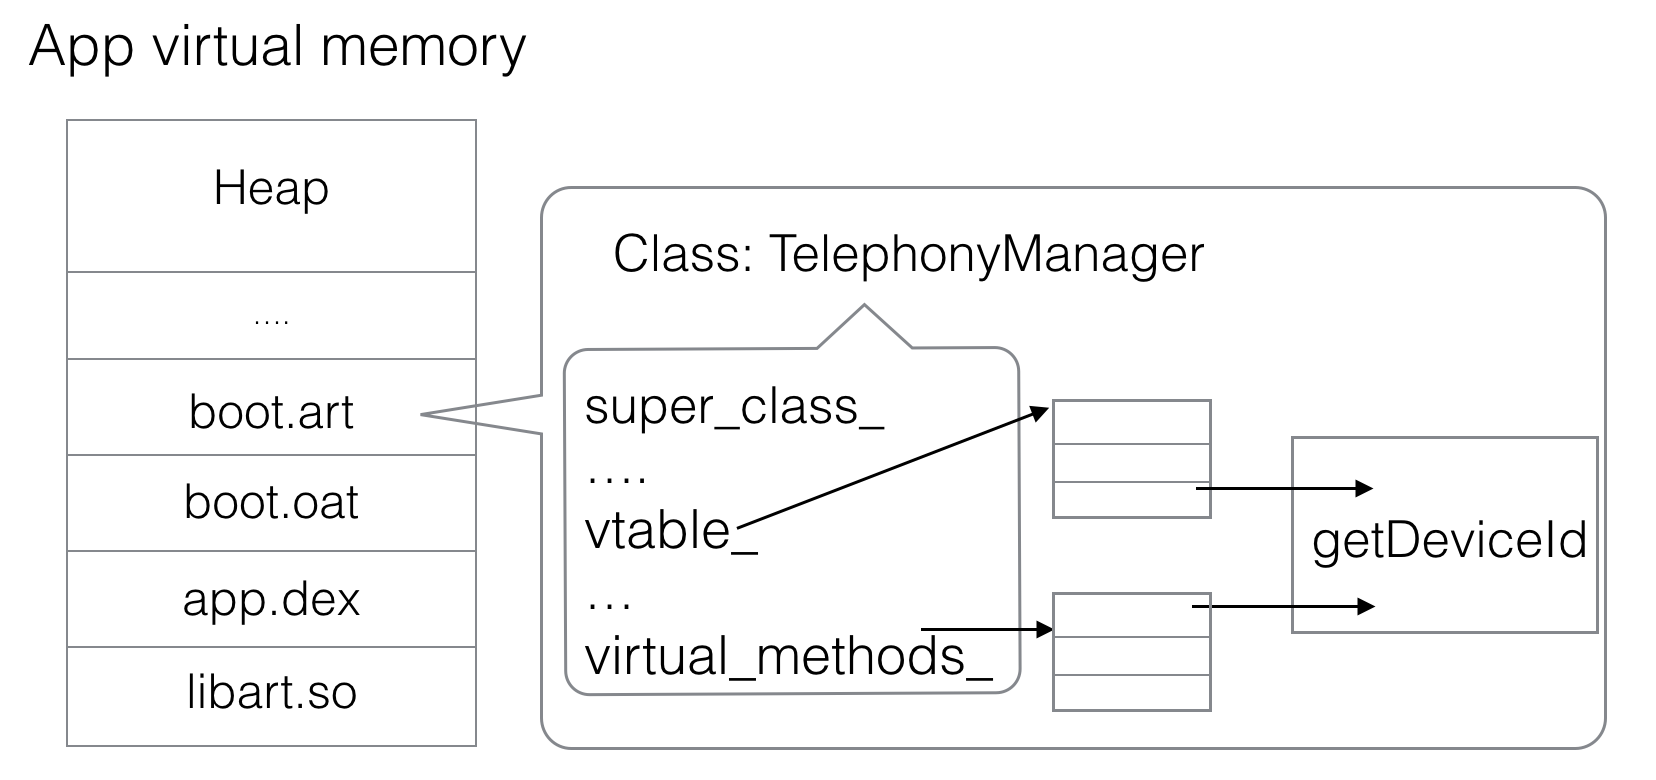
\includegraphics[width=\textwidth]{design1}}
   \subfigure[ARTDroid enabled]{\label{fig:design2}
   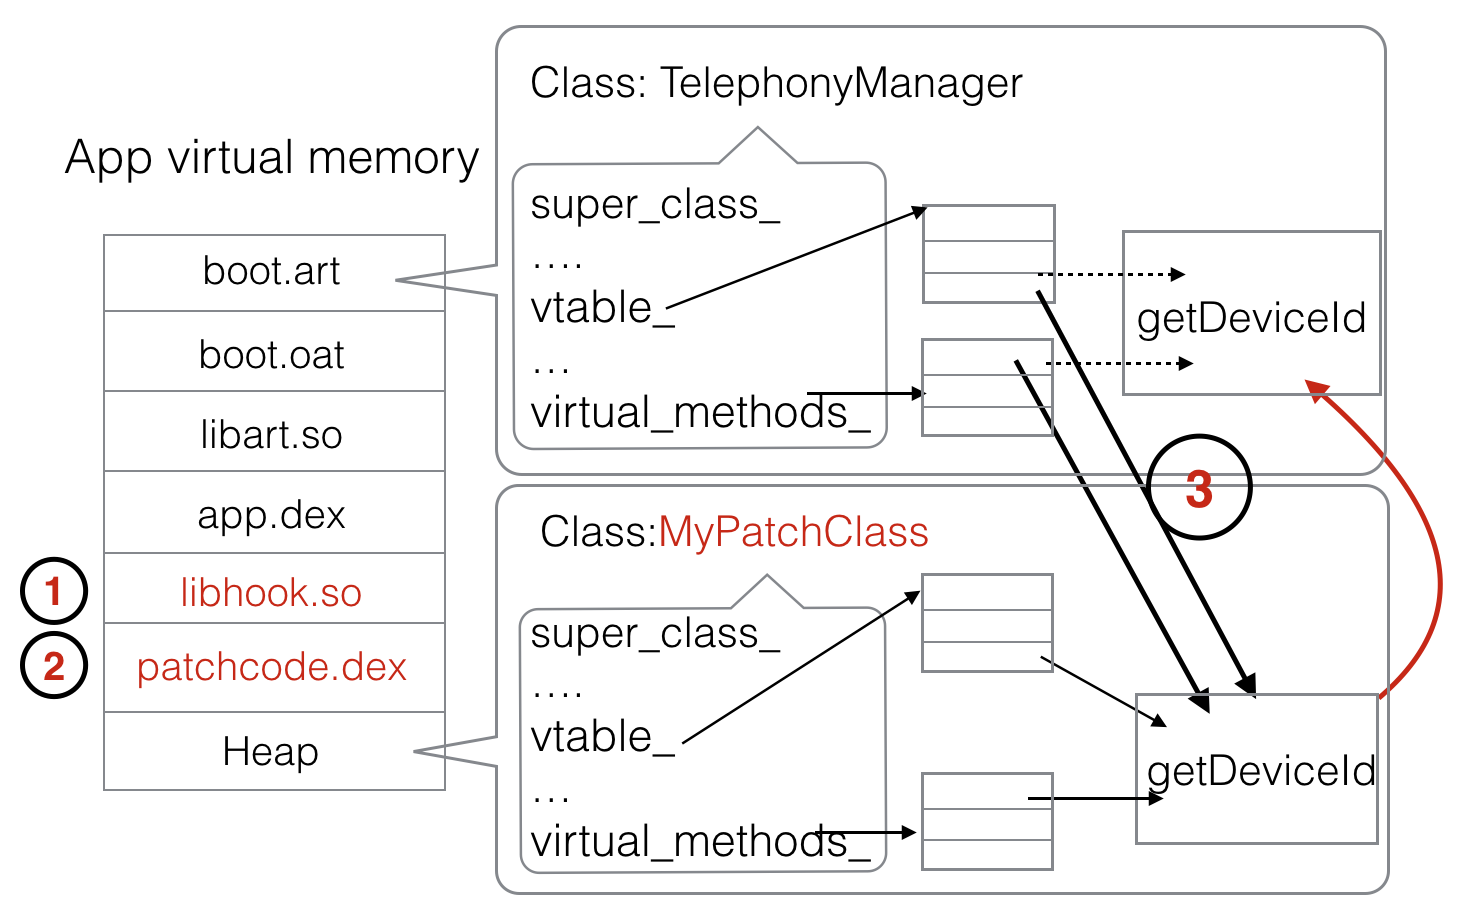
\includegraphics[width=\textwidth]{design2}}
\caption{App virtual memory layout}
\end{figure}



As discussed in \ref{subsub:artinvoke}, the {\tt vtable\_} array is used by the ART runtime to invoke a virtual-method. Instead, the {\tt virtual\_methods\_} array is accessed to return a virtual-method’s reference from memory. ARTDroid exploits these mechanisms to hooking virtual-methods by both {\tt vtable\_ } and {\tt virtual\_methods\_ } hijacking means.



\section{Implementation}
\label{sec:impl}
To get the target method's reference, ARTDroid uses the JNI  function {\tt FindMethodID}. 


ARTDroid overwrites the target method's entry within both the {\tt vtable\_} and {\tt virtual\_methods\_ } array by writing the address of the method's patch code. The original method's reference is not modified by ARTDroid and its address is stored inside the ARTDroid's internal data structures. This address will be used to call the original method implementation. 


When ARTDroid hooks a target method, all calls to that method will be intercepted and they will go to the patch code. Then, the patch code receives the \textit{this} object and the target method's arguments as its parameters. To call the original implementation of target method, ARTDroid exports the function {\tt callOriginalMethod} to the Java patch code. Internally, ARTDroid's core engine calls the original method implementation using the JNI {\tt CallNonVirtual<type>Method} family of routines. These functions can invoke a Java instance method (non-static) on a Java object, according to specified class and methodID.

The original method implementation is invoked by ARTDroid using its address internally stored  before the hooking phase. To guarantee a reliable hooking, ARTDroid uses ADBI features to hook the functions of {\tt CallNonVirtual<type>Method} family. By doing this, all calls to these functions are checked by ARTDroid to block calls to an hooked virtual-method only if these calls do not come from ARTDroid's core engine.


\section{Evaluation}
\label{sec:eva}

\subsection{Performance Test}

To measure the effectiveness of virtual-methods hooking, we firstly need a test set of sensitive methods. SuSi\cite{rasthofer2014machine} provides sensitive methods in Android 4.2. To verify how many of these methods are declared as virtual,  we firstly test them in Android emulator in version 4.2. We use Java reflection to call these methods at runtime. The result of our experiment shows that a remarkable number of virtual-methods could be used to threaten user privacy. The following list describes our experiment results: 

\begin{itemize}
\item 65.1\% of these methods are declared as virtual
\item 6.6\% are non-virtual
\item 28.3\% methods not found
\end{itemize}


Unfortunately, the only methods list available from SuSi is from Android version 4.2. To overcome this limitation, we analyze the sensitive methods list offered by PScout\cite{au2012pscout}. The methods of PScout are available from version 2.2 to version 5.1.1. Our another test is on Android 5.1.1 codebase and it is carried on a Nexus 6 running Android 5.1.1. After analyzing them, we know that only 1.0\% of methods are non-virtual. 

\begin{itemize}
\item 59.2\% of these methods are declared as virtual
\item 1.0\% are non-virtual
\item 39.8\% methods not found
\end{itemize}

However, some methods cannot be found via Java reflection because corresponding classes or methods are not visible to normal apps. They belong to the Android system apps.

So, we can conclude that most of sensitive methods are virtual from our test results. ARTDroid can cover all sensitive methods except 1.0\% methods on Android 5.1.1.



The overhead introduced by ARTDroid depends much on the behavior of the patch code. 

To measure the overhead, we developed a test app, which repeatedly calls sensitive methods or APIs. In particular, this applciation attempts to perform the following operations by calling Android APIs (both via Java reflection and JNI) : initiate several network connections, access sensitive files on the SD card (such as the user's photos), send text message to premium numbers, access the user's contact list and retrive the device's IMEI. 

We used the profiling facilities offered by Android calling the \textit{android.os.Debug}'s \textit{startMethodTracing}/\textit{stopMethodTracing}. Then, the produced traces can be analyzed using either \textit{traceview} or \textit{dmtracedump}. To measure the effective overhead due to ARTDroid, we call the methods using both Java reflection and JNI in addition to the normal invocation. We ran the test 10,000 times for each method, once with ARTdroid disabled and then with ARTDroid enabled mode. The average running time for each call to an hooked method is showed in the following Table \ref{t:perf}.

The most of overhead in ARTDroid is caused by the JNI call, which is internally used to invoke the original method implementation. We registered a worst case overhead of 25\% for each hooked method. Therefore, the total overhead of a call to an hooked method is around 0.25 seconds. This overhead could be decreased by adding an internal cache to store methods' reference called by ARTDroid, instead of using JNI function \textit{FindMethodID}  at each call. We leave these improvements as future work. \\

\begin{table}[ht]
\centering
\caption{Performances}

\bigskip

\begin{tabular}{c  c c c }
\toprule
\multicolumn{1}{c}{ARTDroid} & & Invoke type \\
\cmidrule(r){2-4}
enabled? &  Normal & Reflection & JNI \\ 
\midrule
Yes & 1.12 s   &   1.39 s  &   1.19 s  \\ 
No & 0.88 s& 1.14  s & 0.94 s \\ 
\toprule
overhead & 0.24 s    &   0.25 s  &   0.25 s \\
\toprule
\end{tabular}
\label{t:perf}
\end{table}


\subsection{Case Study}
\label{sec:usage}

Now, we show a case study by hooking \textit{TelephonyManager}'s \textit{getDeviceId} in ARTDroid.

\begin{figure}[ht]
\begin{center}
\lstinputlisting[language=xml]{mysnippets/config.json}
\caption{ARTDroid configuration file}
\label{artconf}
\end{center}
\end{figure}

Figure \ref{artconf} shows the configuration file which contains the definition of methods to hook. 
This file is used to define the information requested by ARTDroid, which are: method's name and signature and the class' name where the patch code is defined in. 
The patch code called instead of method \textit{getDeviceId} is showed inFigure \ref{artpatch}.


\begin{figure}[ht]
\begin{center}
\lstinputlisting[language=Java]{mysnippets/patch-code.java}
\caption{Patch code for method getDeviceId}
\label{artpatch}
\end{center}
\end{figure}

To restore the original call-flow, ARTDroid exposes to Java patch-code the native function {\tt callOriginalMethod}. This function receivers as first argument the string key to identify the target method in the dictionary of hooked methods, internally managed by ARTDroid. Second argument represents the \textit{this} object and the last argument is the array of method's arguments. All future calls to method getDeviceId will be redirected to the patch code, independently if these calls are made using Java reflection mechanisms or JNI.

\section{Discussion}
\label{sec:discuss}

We note that the main goal of our work is to  propose a novel technique to hook Java virtual-methods, our approach can be used to enforce fine-grained user-defined security policies either on real-world devices or emulators as well. Previous research has shown that even benign apps often contain vulnerable components that expose the users to a variety of threaths: common examples are component hijacking vulnerabilities\cite{lu2012chex}, permission leaking \cite{grace2012systematic},\cite{jiang2013detecting} and remote code execution vulnerabilities\cite{poeplau2014execute}.

Suppose the target app is implementing the following features:
\begin{enumerate}
\item \label{itm:first} dynamic code loading
\item\label{itm:second}  code obfuscation (Java reflection, code encryption, etc\ldots)
\item \label{itm:third} integrity checks (i.e, due to copyright issue)
\item \label{itm:fourth} invoke of security-sensitive Java methods via JNI
\item \label{itm:fifth} detection/evasion of emulated environments (i.e, due to copyright issue)
\end{enumerate}

An approach based only on static analysis cannot properly extract security relevant information due to the use of \ref{itm:first}, \ref{itm:second} and \ref{itm:fourth}. Moreover, all existing approaches based on bytecode rewriting techniques cannot analyze that app mainly for the use of integrity checks. Note that since the use of \ref{itm:fifth}, in contrast to ARTDroid, all the existing approaches based on emulated environments can not  properly analyze the behavior of that app. Instead, ARTDroid is still able to analyze that app. Obviously, ARTDroid has its limitations and corner cases. The main limitations is due to the running of the hooking library inside the same process space of the target app. In a scenario where an attacker want to bypass our approach, it can directly invoke a syscall through inline assembly code to gets sensitive results bypassing ARTDroid. We note that the direct system call is not a common technique used by current daily Android malware. Nevertheless, we envise that ARTDroid can be used in conjunction with existing works like \cite{tam2015copperdroid},\cite{zhauniarovich2015stadyna}, \cite{xu2012aurasium}  to provide an additional layer of analysis.



Even though Java direct methods are almost not used for both malicious and security-sensitive behaviors, our future work will support both interface-methods and direct-methods hooking. A possible solution is that we can statically instrument the  {\tt dex2oat} and replace the system original one once we get root privilege. The instrumented {\tt dex2oat} can intercept all interface-methods and direct-methods.

Since ARTDroid hooking library can be injected directly either in Zygote or when the target app is going to be spaw.

Even if the app under testing can tamper with the {\tt vtable\_ }, it can not get the original method's address. In fact, after ARTDroid is enabled, the original method is no more pointed by both the {\tt vtable\_} and {\tt virtual\_methods\_} arrays. 

In section \ref{sec:eva}, we have presented an evaluation about the effectiveness of virtual-methods hooking in the Android system by analyzing results obtained from both SuSi\cite{SuSi} and PScout\cite{au2012pscout} projects. Research results indicate that there is a considerable percentage of sensitive methods which are virtual. Since, ARTDroid can hook virtual-methods and tamper with their arguments, it could be used to define security policies to verifiy apps' behaviors at runtime. For instance, ARTDroid can be used to automatically identify apps which are sending SMS to premium numbers. 

Since the main downside of dynamic analysis techniques is the code-coverage issue, we envise that ARTDroid can be integrated with automatic exploration system like Smartdroid\cite{Zheng:2012}, proposed by Cong et al. 


In the following, we show some applications of ARTDroid:

\begin{itemize}
\item Collect apps behavior at runtime. Analysis of Android API function calls permits the extraction of information about the behavior of apps.
\item Verify security policies at runtime. When users install an app, they can enforce some policies in ARTDroid, so that the new app's sensitive behaviors, such as sending SMS, can be restricted by ARTDroid.
\item Android malware analysis. Some trick malware use a lot of dynamic analysis evading techniques. But in ARTDroid enforced sandbox, our hooking technique cannot be bypassed by current evading techniques. Also, we can easily build our ARTDroid sandbox either on Android emulator or on real devices.
\end{itemize}

\section{Related Work}
\label{sec:related}
Several approaches have been proposed to provide methods hooking on Android. A family of approaches is based on bytecode rewriting technique. The app can be instrumented offline by modifying the app bytecode. AppGuard\cite{backes2013appguard} proposed by Baches et ak, uses this approach to automatically repackage target apps to attach user-level sandboxing and policy enforcement code. Zhou et al. proposed AppCage\cite{zhou2015hybrid}, a system to confine the runtime behavior of the thid-party Android apps. Davis et al. proposed Retroskeleton\cite{davis2013retroskeleton}, an Android app rewriting framework for customizing apps, which is based on their previous work, I-ARM-Droid\cite{davis2012arm}. 


While these approaches are valuable and each of them has its own advantages as well as disadvantages, they have different significant down sides. This approach is not feasible against apps that verify their integrity at runtime. This kind of defense (anti-tampering) is also used in benign apps as well. To be able to replace API-level calls with a secure wrapper, bytecode rewriters need to identify desidered API call-site within the target app. As mentioned in \cite{hao2013effectiveness},\cite{zhauniarovich2015stadyna}, apps that use either Java reflection or dynamically code loading can bypass the app rewriting technique. Moreover, apps which are using JNI to call Java methods can bypass this techniques as well.

A different approach to implement methods tracing can be achieved by using a custom Android system or by using an emulated environment (e.g., a modified QEMU emulator). Enck et al. proposed TaintDroid\cite{enck2014taintdroid}, an Android modified system to detect privacy leak. StayDynA\cite{zhauniarovich2015stadyna} a system for analyzing security of dynamic code loading in Android, uses a custom system image  which can be used only on Nexus like devices. Tam et al. presented CopperDroid\cite{tam2015copperdroid}, a framework built on top of QEMU to automatically perform dynamic analysis of Android malware. These families of approaches, which are based on emulators, can be bypassed by emulation detection techniques \cite{petsas2014rage} \cite{vidas2014evading}. A comparison on Android sanbox has been published by Neuren et al. in \cite{neuner2014enter}. 

Mulliner et al. proposed PatchDroid\cite{mulliner2013patchdroid}, a system to distribute and apply third-party securities patches for Android. This system uses the DDI\cite{DDI} framework. DDI allows to replace arbitrary methods in Dalvik code with native function call using JNI. In \cite{mulliner2014virtualswindle}, Mulliner et. al. shown an automated attack against in-app billing using the DDI capabilities to control the in-app billing purchase flow. Note that the methods used to achieve in-app billing are defined as virtual.

Frida\cite{Frida}, a dynamic code instrumentation toolkit, Xposed framework  \cite{Xposed} and Cydia substrate for Android \cite{Cydia} share similarity with the DDI intrumentation approach. These projects were created for device modding and, in contrast with DDI, require replacing of system components suck as zygote. Currently, Xposed compatibility with ART runtime is actually in beta stage\footnote{\url{http://forum.xda-developers.com/showthread.php?t=3034811}} and the framework installation condition is to flash the device by a custom recovery image.
While these approaches are very suitable under the Dalvik VM, they are totally limited for using under the ART runtime. In fact, both DDI, Frida and Cydia substrate are not able to work under the ART runtime. 

Aurasium \cite{xu2012aurasium} builds a reference monitor into application binaries. The Dalvik code is not patched, but new classes and native code are added to ensure that the instrumentation code is run first. Clearly, such approaches are not effective if the code is obfuscated and protected against static analysis and disassembly. Also note that the package signature of the instrumented applications are broken when they are patched statically. In comparison, our approach does not need to repack the app, our modifications are in-memory only and thus we do not break code signing.

Recent works proposed novel approaches that aim to sandbox unmodified apps in non-rooted devices running stock Android. Boxify\cite{backes2015boxify} presented an approach that aims to sandbox apps by means of syscall interposition (using the ptrace mechanism) and it works by loading and executing the code of the original app within the context of another, monitoring, app. A similar work, \cite{bianchi2015njas} uses the same approach to sandbox arbitrary Android apps. The approach presented in both of these recent works, represent one of the most promising and interesing future work direction.

\section{Chapter Summary}
\label{sec:conclusion}
In this chapter, we presented ARTDroid, a framework for hooking virtual-methods under ART runtime. ARTDroid supports the virtual-method hooking without any modifications to both Android system and app's code. ARTDroid allows to analyze apps even if they employ anti-tampering techniques or they use either Java reflection or JNI to invoke virtual-methods. Moreover, ARTDroid can be used on any real devices with ART runtime once getting the root privilege. The applications of ARTDroid include dynamic analysis of Android malware on real devices or security policies enforcement.










\chapter{StaDART: Combining Static and Dynamic Analysis}
In this chapter, we present StaDART, an extented version of our previously proposed solution Stadyna, which combines static and dynamic analysis of Android applications to reveal the concealed behavior of malware. Unlike Stadyna, StaDART utilizes ArtDroid to avoid modifications to the Android framework. Furthermore, we integrate it with a triggering solution, DroidBot, to make it more scal- able and evaluate it with more Android applications. We present our evaluation results with a dataset of 2,000 real world applications; containing 1,000 legitimate applications and 1,000 malware samples.



\section{Introduction}

Ensuring smartphone users' privacy and security is a major concern and requires adequate measures from app developers, framework providers, and app stores, etc. Google's open source operating system, Android, being the most popular platform for mobile devices, uses Google Bouncer as an app vetting process at its official Google Play store. Vetting processes generally use some form of static/dynamic analysis to scrutinize apps for malicious content and Google Bouncer is no different. In addition, starting from Android 7.0, Android introduced Verify Apps, a new security feature to analyze apps downloaded from sources other than the Google Play store. 

%~\cite{google-bouncer}

However, a growing number of malware samples found in the Android ecosystem reveals that malware developers bypass such vetting processes using various evasion techniques. Previous research shows that the use of dynamic code update techniques along with various forms of obfuscation makes it extremely hard for the state-of-the-art analysis tools to understand the behavior of an app\cite{ExecuteThis_Poeplau2014, ahmad2016empirical}. Thus, the use of these evasion techniques in newly found malware is not surprising~\cite{brain-test}. This paper provides an empirical demonstration of the lack of effectiveness of the state-of-the-art tools when it comes to analysing apps that hide suspicious behavior using reflection and dynamic code loading. We develop a set of benchmark apps that use reflection in different ways to conceal information leakage. Our analysis of reflection-bench using some of the state-of-the-art static analysis tools shows their ineffectiveness to handle apps that use reflection. Furthermore, we develop InboxArchiver, a seemingly benign app that uses dynamic code loading to hide its suspicious functionality, and use it to test some of the most well known online analysis services. The analysis show that InboxArchiver easily bypasses these security analysis services. %\footnote{Similar proof of concept apps, which were able to 

Static analysis relies on the availability of all the information at analysis time, hence, it suffers  from dynamic features and unavailability of information that are known only at execution time, e.g., the parameters used in the dynamic code update APIs. Therefore, reflection that is a programming technique widely used by mobile app developers can be only partially investigated by current  static analysis tools. As a result, reflection is usually used by malware developers to hide malicious code. The inherent limitation of  all static analyzers  (e.g., \cite{FlowDroid_Arzt2014,Saaf_Hoffmann2013}) is the operational assumption  that the code base does not change dynamically and the targets of reflection calls can be discovered in advance. This is a clear simplification of what happens in the real world, where many apps rely on code base updates instantiated only at runtime.


There exist approaches that enhanced static analyzers of Java code to deal with the presence of dynamic code update techniques (e.g., \cite{TamingReflection_Bodden2011}). However, they cannot be  applied directly to Android due to the differences in the Java and Android platforms. The alternative of instrumenting the app offline has the  major drawback of breaking the app signature, that some apps check  at runtime. As the app starts, it checks the integrity of the signature against  a  value hardcoded in the app and terminates if the check fails. In case of malicious apps this check may be used to conceal illicit behavior. 

In this paper, we present StaDART, a mobile app security analysis tool that combines static and dynamic analysis to address the presence of dynamic code updates. Instead of relying on modifications to the Android framework, StaDART utilizes a vtable tampering technique for API hooking to perform dynamic instrumentation~\cite{costamagna2016artdroid}. Furthermore, we integrate StaDART with DroidBot, a triggering tool for Android apps, to make the analysis  fully automated. StaDART is evaluated using a dataset of 2,000 real world apps (both malicious and benign) and the results of our evaluation reveal that it is more common in malicious apps to use dynamic code updates to conceal malicious behavior which is only exhibited once the app is installed on a real device. Moreover, 33\% of malware samples that use DCL introduce APIs guarded with new (not used in the initial code base) dangerous permissions in the newly loaded code, whereas the analysed benign apps do not exhibit such behavior.  

\textbf{Contributions:}

\begin{itemize}
\item We present the design and implementation of StaDART, a system that interleaves static and dynamic analysis in order to reveal the hidden/updated behavior of Android apps. By utilizing vtable tampering for API hooking, we avoid modifications to the Android framework and make it largely framework independent. StaDART analyzes the code loaded dynamically, and is able to resolve the targets of reflective calls complementing app's method call graph with the obtained information. Therefore, StaDART can be used in conjunction with other static analyzers to make their analysis more accurate.

\item We integrate StaDART with DroidBot to make it fully automated and to ease the evaluation. Moreover, we analyze a dataset of 2,000 real world apps (1,000 benign and 1,000 malicious). Our analysis results show the effectiveness of StaDART in revealing behavior which is otherwise hidden to static analysis tools.  

\item We release our tool as open-source to drive the research on app analysis in the presence of dynamic code updates.
%\footnote{\url{new link}}
\item We design and develop reflection-bench, a set of benchmark apps that use reflection to conceal information leakage, and use it to test some of the state-of-the-art static analysis tools. We publish reflection-bench so that researchers can test the effectiveness of their analysis tools in the presence of dynamic features (i.e., reflection). 

\end{itemize}

\textbf{Paper Organization:}

\S\ref{sec:info_android} provides a background on dynamic class loading and reflection in Android. 
\S\ref{sec:refbench_dcl} discusses the design and implementation details of reflection-bench and InboxArchiver. It also provides the analysis results highlighting the shortcomings of state-of-the-art Android app analysis tools. \S\ref{sec::system_general_description} gives a high-level description of StaDART, while \S\ref{sec::implementation} covers the implementation details. \S \ref{sec:mcg_description} presents our approach to build method call graphs and visualise them. \S\ref{sec:evaluation} reports the evaluation results of StaDART on real world apps. \S\ref{sec:discussion} discusses the limitations of the current implementation, and envisages the future work. \S\ref{sec:relwork} overviews the related work, and \S\ref{sec:conclusion} concludes the paper.


%%%%%%%%%%%%%%%%%%%%%%%%%%%%%%%%%%%%%%%%%%%%%%%%%%%%%%%%%%%%%%%%%%%%%%%%%%%%%%%%%%%%%%%%%%%%
\section{Motivating example}
\label{sec:prob}

% In the last year, several applications have been removed from the GooglePlay store due to their malicious behavior. Moreover, malware authors have started to improve the techniques used in their product to hide its malicious behavior by means of either obfuscation or dynamic code loading capabilities. 

%have started to improve the techniques used in their product to hide its malicious behavior by means of either obfuscation or dynamic code loading capabilities. 
%Therefore, they cannot detect suspicious data passed in via an Intent between two different Android components.

The rising use of techniques such as obfuscation and ICC for information leakage by newly found malware motivates this work. Existing analysis approaches generally do not support information-flow analysis across multiple app components in obfuscated apps. As a result, malware use these features for evading these analysis tools. As reported by different antivirus companies \cite{acecard,adware,adwaregplay,vbmalware,rumms}, obfuscated malware has started to show up more frequently. This trend poses a strong challenge for the current static analysis tools, which are unable to automatically analyze apps in the presence of obfuscation or dynamic code loading. Furthermore, as demonstrated in \cite{li2015iccta}, the ICC mechanism offered by Android is used by both normal and malicious apps for passing data between different Android components. 
%\cite{parasites},
% Beside that, current state of the art tool based on hybrid approach \cite{backes2016r,rasthofer2016harvesting} are not able to automatically detect suspicious flows between different components due to the lack of support for ICC. 
%Our hybrid approach, like \cite{backes2016r,rasthofer2016harvesting}, follows the process of extract-then-execute interesting code extracted 



\iffalse
\begin{figure}[ht!]
\centering
\lstinputlisting[language=Java,label={lst:test1}]{listings/malware1.java}
\caption{MessageReceiver}
\label{fig:mlw1}
\end{figure}
\fi

\lstinputlisting[language=Java,label={lst:m1w1}, caption={MessageReceiver}]{listings/malware1.java}

\iffalse
\begin{figure}[ht!]
\centering
\lstinputlisting[language=Java,label={lst:test1}]{listings/malware2.java}
\caption{SendService}
\label{fig:mlw2}
\end{figure}
\fi

\lstinputlisting[language=Java,label={lst:m1w2}, caption={SendService}]{listings/malware2.java}

To ease the understanding of our contributions, we are going to introduce a code snippet of a real-malware sample reported by FireEye in \cite{firemalware}. Listing \ref{lst:m1w1} shows the de-obfuscated version of the code used to intercept and then report the incoming SMS. The forwarding process is defined in a service component. The \emph{MessageReceiver} (line 2) is called for each incoming SMS and then an Android service is started by an Intent (line 12). The number and text data are stored within the Intent (lines 10, 11). Note that the original obfuscated malware uses string encryption on the constant string along with Java reflection for calling ICC methods. Then the started service, shown in Listing \ref{lst:m1w2}, gets data from the incoming Intent (lines 5, 6) and leaks (line 14) SMS number and text via a remote server connection (the server IP address string was obfuscated as well).

% TOOLNAME permits to automatically extract and then execute the relevant instructions which compute the value at the POI. The ICC flow is first detected to build the SDG and then used to  drive the backward-slicer across different components. Moreover, TOOLNAME automatically detect the component's type where the backward-slicing process ends.  This information is used along with the Manifest data, to automatically trigger specific system events (i.e., incoming sms, etc\ldots).

To the best of our understanding, static analyzers \cite{octeau2013effective,octeau2015composite,li2015iccta,gordon2015information}, are not successful in analyzing such cases because of both encryption and reflection techniques used by this malware sample. Moreover, also hybrid approaches proposed in \cite{rasthofer2016harvesting} and \cite{backes2016r} cannot properly analyze the sample because they lack support for ICC. 

%In the following section we describe how our iterative approach based on a combination of static and dynamic analysis can solve the problem.



% Listing \ref{fig:outact},\ref{fig:inact} show code snippets taken from DroidBench \cite{droidbenchpage} suite. It is an open test suite for evaluating the effectiveness of taint-analysis tools. It is, basically, a collection of several  apps which leak sensitive data exploiting different Android features (like Android activity lifecycle, callback, thread, ICC, etc\ldots). Even if it is mainly intended for a different purpose (the evaluation of taint-analysis tools), in the following we are going to use ICC-base Droidbench apps (included in \emph{InterComponentCommunication} test case) to ease the understanding of our approach. We obfuscated those apps using the Dexguard \cite{dexguardpage} tool exploiting different techniques like Java reflection and string encryption. Then, instead of looking for a flow between source and sink methods, our goal is to automatically extract the malicious behavior, which involves ICC mechanism, from the obfuscated app.

% \begin{figure}[ht!]
% \centering
% \subfigure[Multiple Method Slice]{
% \centering
% \lstinputlisting[language=Java,label={lst:test1}]{listings/ActComm7.java}
% \label{fig:outact}
% }
% ~%Nothing
% \subfigure[Inline Slices]{
% \centering
% \lstinputlisting[language=Java,label={lst:test1}]{listings/ActComm7_2.java}
% \label{fig:inact}
% }
% %~%Nothing
% %\subfigure[Inline Slices]{
% %\centering
% %\lstinputlisting[language=Java,label=%{lst:test1}]{listings/ActComm7_3.java}
% %\label{fig:slices}
% %}
% \caption{Slice Categories; \textit{E}: Entrypoint Method, \textit{T}: Target Method, \textit{IM}: Intermediate Method, \textit{NR}: Non-relevant Method}
% \label{fig:slice_categories}
% \end{figure}

% Listing \ref{fig:outact},\ref{fig:inact} illustrate two Activities. \emph{OutFlowActivity} which first gets a sensitive data (the IMEI number, line 7 Listing \ref{fig:outact} ) then send it to the Activity \emph{InFlowActivity}. Finally, it does data exfiltration via SMS vector (line 9 \ref{fig:inact}. The obfuscation by Dexguard encrypts the string in both Activities (lines 11,13 and 6,9) with a call to method \emph{f.e} passing in the encrypted string as argument. Moreover, Listing \ref{fig:outact} line 13, the call to startActivity method has been replaced with an indirect call via Java reflection mechanism.
% The intent created at line 9 is exchanged between the two components by first attach the data using putExtra (line 11) method and then by invoking the ICC method startActivity (line 13).


% As discussed before, all existing approaches \cite{octeau2015composite,octeau2013effective,rasthofer2016harvesting,li2015iccta,backes2016r} fail the analysis because either they can not detect flow between different Android components, or because of its obfuscation. This consideration holds for hybrid approaches like Harvester \cite{rasthofer2016harvesting} and R-Droid \cite{backes2016r} as well. Both of them will also fail in the analysis because they can not properly follow ICC flows. 

%However, our approach XXX allows the extraction of data-dependent slices following the ICC flow across the two Activities. Listing \ref{fig:slices} shows the resulting slice generated by XXX, it shows the corresponding aggregate Java code to ease the understanding.
%XXX performs backward slicing starting from the POI, sendTextMessage method, looking for data-dependency on both the first and third arguments (respectively message's number and body). The instructions which are linked with that arguments are added during the slicing process. Finally, only the instructions which participate in the computation of the target arguments are included in the resulting slice, Listing \ref{fig:slices}. 


% It is often desired to dynamically execute an application to test it for possible errors, vulnerabilities and malicious activities. Checking an app for possible malicious activities is one of the foremost duties of an app store. More specifically, an app store is required to make sure that the published apps are free of malicious contents. Therefore, app stores do have some sort of scanning mechanism which analyzes apps statically/dynamically.

% Static analysis most of the times provides an over approximation of the behavior of an app under test. So, static analysis might declare an app malicious which might be benign. In contrast, the behavior of an app estimated using dynamic analysis provides an exact idea about what an app is capable of doing. However, dynamic analysis requires to stimulate an app with proper test cases which could expose the complete behavior of the app, which is most of the times ungainly and does not scale well due to the huge number of the apps.

% However, it is some times more desirable to stimulate only specific parts of an app and not the app as whole, e.g., some sensitive APIs which access phone resources or send data to the outside world, some pieces of code which may produce errors, some specific APIs which update the app's code dynamically, etc. This gives rise to the problem of generating targeted test cases which could stimulate the desired target piece of code. 



% This work aims to solve the mentioned problem and contributes as listed below.
% \begin{itemize}

% \item A novel idea which could move forward the state-of-the-art in targeted triggering. The idea is to move towards environment independent targeted triggering rather than providing the exact environment/inputs required for triggering, i.e., instrument/enrich the app in a manner that makes it take the required paths when launched.

% \item Design and implement an automated system, TExeDroid for Android apps based on the proposed idea which takes an APK file and a list of target APIs and ensures that the code path leading to these target APIs are stimulated while dynamically executing the app on a device or an emulator.

% \item TExeDroid can be easily coupled with state-of-the-art dynamic analysis tools to get better results. As a use case, we couple TExeDroid with StaDyna to resolve the targets of reflection and dynamic code loading for capturing the runtime behavior of Android apps.

% \item We collect a dataset of X Android apps (containing  X1 malicious and X2 benign apps). We evaluate TExeDroid with the collected dataset of apps and report our findings.

% \end{itemize}

%\item Most of the tools for analyzing Android apps are based on their counterparts developed for Java applications and therefore, the Dalvik bytecode of Android apps needs to be translated to Java bytecode for analysis. The state-of-the-art tools for translating Dalvik bytecode to Java bytecode are not very much matured. Therefore, we try to perform all the analysis on a Smali level (a closer and more precise representation of the Dalvik bytecode). Performing all the analysis on Smali level leads to a more accurate and a less expensive solution.



% %%%%%%%%%%%%%%%%%%%%%%%%%%%%%%%%%%%%%%%%%%%%%%%%%%%%%%%%%%%%%%%%%%%%%%%%%%%%%%%%%%%%%%%%%%%%
\section{Our approach}
\label{sec:our_approach}

\begin{figure*}[ht!]
\centering
\subfigure[SDG - First Iteration]{
\centering
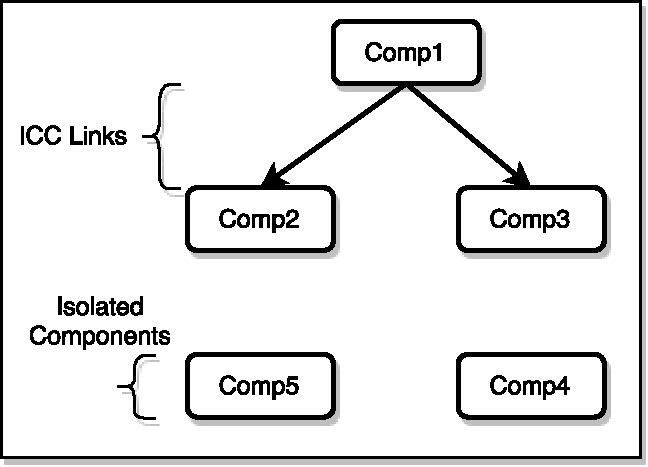
\includegraphics[scale=0.47]{SDG1}
\label{fig:sdg1}
}%
~%Nothing
\subfigure[SDG - Second Iteration]{
\centering
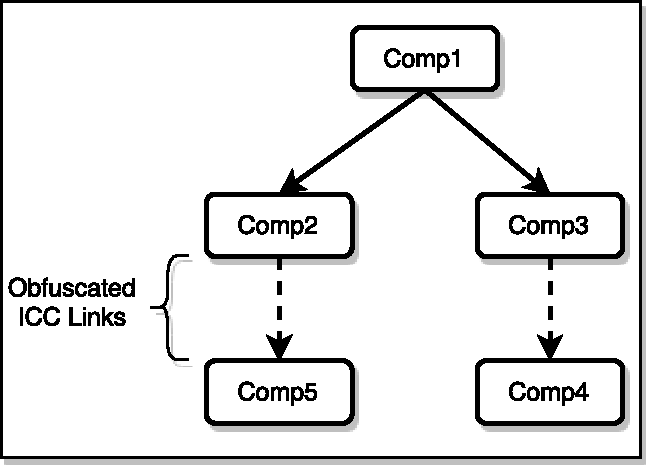
\includegraphics[scale=0.47]{SDG2}
\label{fig:sdg2}
}%
\caption{SDG during the first and second iteration. Comp: Component}
\label{fig:sdg}

\end{figure*}

During a normal execution of an Android app, the control transfers between various components based on certain user or system events. In order to trigger a specific piece of code inside an app, it is important to provide the exact user/system events in a specific order to make it follow the target path. We take a slightly different approach based on isolating target execution paths from within the app and executing them; thereby avoiding to rely on user/system events. Target execution paths are isolated by means of a slice extraction mechanism that leverages backward program slicing across various components of the app.  

\subsection{Slice Extraction}

Backward code slicing is a static analysis technique that identifies the data flow to a certain variable \textit{v} at point \textit{p} in the program while tracking the code in backward direction. In the process it identifies all the code instructions \textit{I} which directly or indirectly affect the value of \textit{v} at point \textit{p}. This set of instructions \textit{I} is called a backward slice. An important property of a backward slice is that it can execute independently of the rest of the program. 

We leverage this property of the backward slice in our approach. Our backward slicing mechanism starts from a target point and traverses the code in backward direction until it reaches an entry point in the app. Instructions corresponding to each target point are marked accordingly and extracted from the program to be refined and executed separately. In simple apps, a backward slice may belong to a single app component. However, the complexity of apps these days demands for more inter component communication. Therefore, approaches based on extracting slices from only a single component might miss critical information passed through ICC.  

\subsection{Inter-Component Communication}

Our approach extends backward slicing across multiple app components. We build a System Dependency Graph (SDG) before starting slice extraction. A SDG is a representation of the program highlighting the inter-connectivity and program flow among various components. Figure~\ref{fig:sdg} provides a simplified representation of a SDG. The \textit{nodes} in the SDG represent components which are connected to each other with directed \textit{edges} where the direction shows the flow of execution from one component to the other. A SDG also provides information about the nature of the components, \textit{i.e.}, activity, service, broadcast receiver, etc. This information is not shown in the figure where we simply refer to them as Comp\textit{X}. The backward slicing assisted by the SDG then extracts slices which may contain instructions from multiple components. 

\iffalse
\begin{figure}[ht!]
\centering
\lstinputlisting[language=Java,label={lst:test1}]{listings/slice.java}
\label{fig:slices}
\caption{Extracted and Refined Slice}
\label{fig:slices}
\end{figure}
\fi

\lstinputlisting[language=Java,label={lst:slices}, caption={Extracted and Refined Slice}]{listings/slice.java}

%Listing \ref{fig:outact} and \ref{fig:inact} show code snippets taken from DroidBench \cite{droidbenchpage} suite. It is an open test suite for evaluating the effectiveness of taint-analysis tools. It is, basically, a collection of several  apps which leak sensitive data exploiting different Android features (like Android activity lifecycle, callback, thread, ICC, etc\ldots). Even if it is mainly intended for a different purpose (the evaluation of taint-analysis tools), in the following we used an example app from Droidbench (the ones which uses ICC for malicious behavior) to describe and demonstrate the effectiveness of our approach. We used the Dexguard \cite{dexguardpage} tool to obfuscate the interesting apps using different techniques like Java reflection and string encryption. Then, instead of looking for a flow between source and sink methods, our goal is to automatically extract the malicious behavior, which involves ICC mechanism, from the obfuscated app.

Our approach uses an iterative mechanism which works in a CreateSDG-ExtractSlice-Execute cycle. Each phase in this cycle provides input for the next phase. SDGs help in extracting slices across multiple components and extracted slices simplify execution of target points in the app. Similarly, the execution phase helps in resolving obfuscation and dynamic code updates which leads to improved creation of the SDG in the next iteration. Figure~\ref{fig:sdg1} and \ref{fig:sdg2} show a SDG in two iterations. In the first iteration, TeICC finds the obvious non-obfuscated ICC links only. Therefore, the SDG contains Comp4 and Comp5 which are isolated components. The second iteration reveals that the app has obfuscated ICC links from Comp2 to Comp5 and from Comp3 to Comp4 as shown in Figure~\ref{fig:sdg2}. This process carries on until the SDG reaches a stable point. At this stage, all the obfuscated links are resolved and the slices are ready for the final execution to capture and analyze suspicious behavior.

%Listing \ref{fig:outact} and \ref{fig:inact} illustrate two Activities. OutFlowActivity which first gets a sensitive data (the IMEI number, line 7 Listing \ref{fig:outact} ) then send it to the second Activity: InFlowActivity. Finally, it does data exfiltration via the SMS vector (line 9 \ref{fig:inact}. The obfuscation by Dexguard encrypts the string in both Activities (lines 11, 13 and 6, 9) with a call to f.e method passing in as argument the encrypted string. Moreover, Listing \ref{fig:outact} line 13, the call to startActivity method has been replaced with an indirect call via Java reflection mechanism. The Intent is created at line 9, then that intent is exchanged between the two components by first attach the data using putExtra (line 11) method and then by invoking the ICC method startActivity (line 13).

%At the best of our knowledge, static analyzers like IC3 \cite{octeau2015composite} and EPICC \cite{octeau2013effective} will fail because of both encryption and reflection techniques. Moreover, also hybrid approaches proposed in \cite{rasthofer2015harvesting} and \cite{backes2016r} fail as well, because they lack support of ICC.

% As discussed before, all existing approaches \cite{octeau2015composite,octeau2013effective,rasthofer2016harvesting,li2015iccta,backes2016r} fail the analysis because either they can not detect flow between different Android components, or because of its obfuscation. This consideration holds for hybrid approaches like Harvester \cite{rasthofer2016harvesting} and R-Droid \cite{backes2016r} as well. Both of them will also fail in the analysis because they can not properly follow ICC flows. 

Most of the state-of-the-art analysis tools would fail to extract the complete slice in the case of the sample described in \S\ref{sec:prob}. However, TeICC allows the extraction of such data-dependent slices because it can follow the ICC flow across multiple components. Listing \ref{lst:slices} shows the resulting slice extracted and refined by TeICC; it shows the corresponding aggregated Java code to ease the understanding. 
%TeICC performs backward slicing starting from a MOI looking for data-dependency. The instructions which are linked with the  MOI are added during the slicing process. Finally, only the instructions which participate in the computation of the target arguments in the MOI are included in the resulting slice, Listing \ref{fig:slices}.

\subsection{Slice Execution}

The extracted slices are put together in one or more resultant components where the irrelevant instructions are removed as shown in Listing~\ref{lst:slices}. Similarly, the \texttt{AndroidManifest.xml} file is also modified to include entries for these resultant components and remove irrelevant ones. The enriched app is then assembled and signed. The flow of the app is hijacked using a stub code so that it executes the resultant component after it is launched. The app is then installed and run on a real device or emulator. The target slice is executed once the resultant component is started. Similarly for each extracted slice, a resultant component is added to the app. The app is observed during execution of the resultant components to capture the target behavior of the app. 

% Android apps are composed of various components where the execution moves from one component to another when it receives certain user or system events. In order to trigger a specific piece of code inside an application, an exact environment needs to be provided. An exact environment may include a number of things, such as a specific OS, specific libraries, real device or emulator, internet connectivity, specific date and time, specific user/system events and so on, depending upon the app. Therefore, different apps require different execution environments. Providing a generic environment which could work with every application is not feasible. To overcome this problem, our new approach is based on removing the environment dependency required for triggering instead of providing the environment. We try to modify the application in such a way that it no more requires triggers from the outside world to execute specific portions of the code. In the following subsections, we provide a step wise explanation of our approach.

% \subsection{Slice Extraction and Categorization}


% In order to reach a specific point in the code, the application must be executed in a such way that it takes the path from an entry point to the target point. Therefore, it is important to identify the path from the entry point to the target. To a larger extent, such path can be identified in an application using some static analysis techniques. Our targeted dynamic triggering solution is also backed by static analysis. In the static analysis phase, a static analyzer identifies the targets in the application. The static analyzer is then used to perform backward slicing of the application to extract the paths composed of code statements starting at an entry point and leading to the identified target. These are the code statements which directly or indirectly influence the instruction in the target code line. Table \ref{tab:single_method_slice} shows an example of a slice. In order to facilitate further analysis, we divide the execution paths/code slices into different categories.

% %In this case, we use a modified version of SAAF (Static Android Analysis Framework) as a static analyzer.

% \textbf{SingleMethod:} Depending upon the depth and the position of the target code line, a slice may contain code statements from one or multiple methods. A single method slice is one which contains statements belonging to only one method. Table \ref{tab:single_method_slice} shows an example of a single method slice where all the statements belong to the \texttt{onCreate} method of the \texttt{wap.syst.activity} class. The first column in the table represents the slice \textit{ID}. Each slice is assigned a unique ID starting from zero, which increments for each new slice corresponding to a new target. The next three columns, \textit{TLine\#}, \textit{TClass} and \textit{TMethod}, represent the target line number, target class and target method, respectively. The column \textit{CClass} represents the class containing the current code line, whereas, the corresponding method is represented by column \textit{CMethod}. The last column contains the code lines including their line numbers and instructions.

% \todo[inline]{Correct the line numbers in the table}

% \begin{table*}[t!]
% \centering
% \caption{Single Method Slice}
% \label{tab:single_method_slice}

% \scriptsize

% \begin{tabular}{|c|c|c|c|c|c|p{6cm}|}
% \hline
% \textbf{ID} & \textbf{TLine\#} & \textbf{TClass} & \textbf{TMethod} & \textbf{CClass} & \textbf{CMethod} & \textbf{CodeLine} \\
% \hline
% \hline

% 0 & 19 & \texttt{wap.syst.activity} & onCreate & \texttt{wap.syst.activity} & onCreate & \texttt{59: move-result-object v1}\\
% 0 & 19 & \texttt{wap.syst.activity} & onCreate & \texttt{wap.syst.activity} & onCreate & \texttt{55: const-string v12, class}\\
% 0 & 19 & \texttt{wap.syst.activity} & onCreate & \texttt{wap.syst.activity} & onCreate & \texttt{52: invoke-virtual {v9, v10}, Ljava/util/Properties;->load(Ljava/io/InputStream;)V}\\
% 0 & 19 & \texttt{wap.syst.activity} & onCreate & \texttt{wap.syst.activity} & onCreate & \texttt{48: invoke-direct {v9}, Ljava/util/Properties;-><init>()V}\\
% 0 & 19 & \texttt{wap.syst.activity} & onCreate & \texttt{wap.syst.activity} & onCreate & \texttt{46: new-instance v9, Ljava/util/Properties;}\\
% 0 & 19 & \texttt{wap.syst.activity} & onCreate & \texttt{wap.syst.activity} & onCreate & \texttt{42: move-result-object v10}\\
% 0 & 19 & \texttt{wap.syst.activity} & onCreate & \texttt{wap.syst.activity} & onCreate & \texttt{38: const/high16 v13, 0x7f05}\\
% 0 & 19 & \texttt{wap.syst.activity} & onCreate & \texttt{wap.syst.activity} & onCreate & \texttt{59: move-result-object v12}\\
% \hline

% \end{tabular}
% \end{table*}


% \textbf{MultipleMethods:} A more usual case will be a multiple method slice which is composed of multiple methods and contains transitions from one method to the other at specific points. Where a single method slice can be triggered fairly easily, the multiple method slices are hard to trigger as the transition might be dependent upon some user/system events or a particular state of some environment variables. Figure \ref{fig:multiple_method_slice} shows an example of a composite slice. The blocks represent methods and the arrows represent transitions from one method to anther method. A slice starts with an \textit{entrypoint} method and ends at a \textit{target} method. The control flows through a number of \textit{intermediate} methods before reaching the target. In Figure \ref{fig:multiple_method_slice}, the methods which are part of the target slice are encapsulated in a box and shaded grey.



% %\begin{figure}[h!]
% %\centering
% %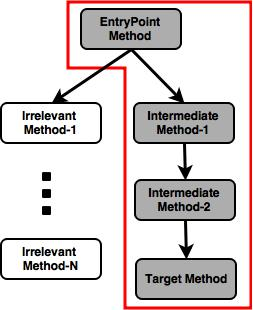
\includegraphics[scale=0.6]{MultipleMethodSlice}
% %\caption{Multiple Method Slice}
% %\label{fig:multiple_method_slice}
% %\end{figure}

% \begin{figure*}[t!]
% \centering
% \subfigure[Multiple Method Slice]{
% \centering
% 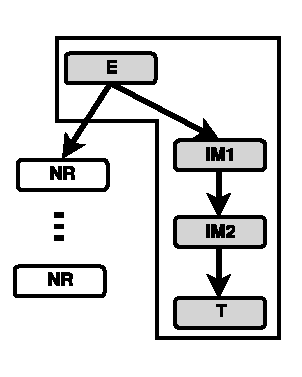
\includegraphics[scale=0.7]{MultipleMethodSliceTExeD.pdf} %[width=.25\textwidth]
% \label{fig:multiple_method_slice}
% }
% ~%Nothing
% \subfigure[Inline Slices]{
% \centering
% 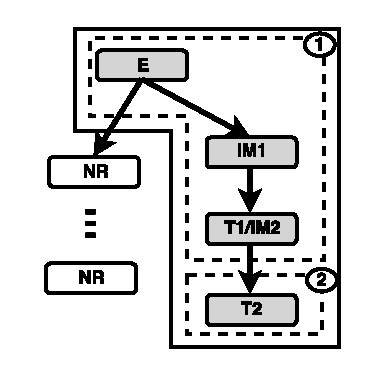
\includegraphics[scale=0.7]{InlineSlicesTExeD.pdf}
% \label{fig:inline_slices}
% }
% ~%Nothing
% \subfigure[Composite Slice]{
% \centering
% 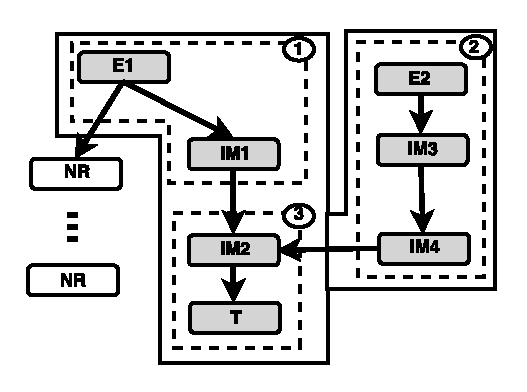
\includegraphics[scale=0.7]{CompositeSliceTExeD.pdf}
% \label{fig:composite_slice}
% }
% \caption{Slice Categories; \textit{E}: Entrypoint Method, \textit{T}: Target Method, \textit{IM}: Intermediate Method, \textit{NR}: Non-relevant Method}
% \label{fig:slice_categories}
% \end{figure*}


% \textbf{InlineSlice:} Inline slices are those slices where one slice is a sub-slice of the other slice. In this case, the targets lie on the same execution path. Therefore, such slices can be triggered in one execution. Figure\ref{fig:inline_slices} shows two such inline slices where the slice encapsulated in the dashed box \circled{1} is a sub-slice of the slice encapsulated in the solid box. The target of first is slice \textit{T1} which serves as an intermediate method for the target \textit{T2}. This can be the case where the target slices represent dynamic class loading and reflection APIs. Usually, additional code is loaded using dynamic class loading APIs and its methods are invoked using reflection APIs. Ideally, this should be a perfect case of inline slices.

% %\begin{figure}[h!]
% %\centering
% %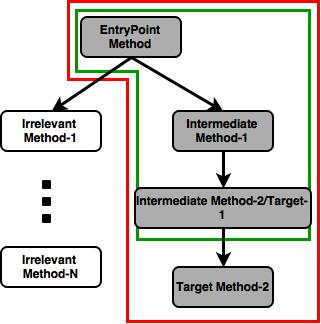
\includegraphics[scale=0.6]{InlineSlices}
% %\caption{Inline Slices}
% %\label{fig:inline_slices}
% %\end{figure}



% \textbf{CompositeSlice:} A target code line, usually an API call, may contain more than one parameters where the flow of information to these parameters could be through different execution paths. Therefore, the corresponding target slice is a combination of multiple distinct slices. Slices corresponding the same target code line combine together to form a composite slice encapsulated in a solid box as shown in Figure\ref{fig:composite_slice}.

% %A backward slice in an application corresponds to a specific pattern where a pattern can be an API call with a specific parameter. Therefore, an API call having multiple interesting parameters would form multiple patterns and thus, result in multiple slices. The next step is to find such slices for each API call invokation instance. There is a unique \textit{ID} for every pattern. However, slices with different \textit{ID}s can be dealt with together if they correspond to the same target code line. Slices corresponding the same target code line combine together to form a composite slice encapsulated in a red box as shown in Figure\ref{fig:composite_slice}.

% %\begin{figure}[h!]
% %\centering
% %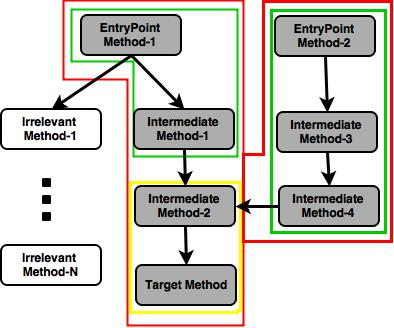
\includegraphics[scale=0.6]{CompositeSlice}
% %\caption{Composite Slice}
% %\label{fig:composite_slice}
% %\end{figure}

% To make things simpler, a composite slice is divided into multiple sub-slices. Among these slices, the common and uncommon portions are separated. Since all these slices end up at the same target line, the latter portion of these slices is more likely to be the common portion, called \textit{CommonSlice} which is encapsulated in the dashed box \circled{3} in Figure\ref{fig:composite_slice}. The uncommon portions in these slices are treated as separate slices, called \textit{PartialSlice}s. In Figure\ref{fig:composite_slice}, partial slices are encapsulated in dashed boxes \circled{1} and \circled{2}. Separation of these slices helps in a making sure that \textit{PartialSlice}s get executed before the \textit{CommonSlice} in this case.

% %Where does the uncommon portion come from? Is it the same method? Or different? If different, whether coming from some eventListener or normal method? Deal the uncommon portions of the slice as different slices. Internally connected using the duplicate/stitch method. N from the outside,
% %MainActivity->PartialSlice1
% %return->MainActivity->ParticalSlice2
% %return->MainActivity->CommonSlice



% %\subsection{Critical Points Identification}
% \subsection{Analyzing Transitions}

% In a multiple method slice, the statements belong to more than one methods and may belong to more than one classes where the transitions from one method to another method can be an explicit one or an implicit one. The identification of such transition points and their nature in the slice are essential in triggering the app along the target slice.

% \begin{lstlisting}[language=java, label={lst:m1tom2}, caption={method1 to method2}]
% .method public method1()V
%  .registers 1
%  .prologue
%  .line 19
%  invoke-virtual {p0}, Ldisi/unitn/targettriger/testapp/MainActivity;->method2()V
%  .line 20
%  return-void
%  .end method
% \end{lstlisting}

% \begin{lstlisting}[language=java, label={lst:m2tom1}, caption={method2 to method1}]
%  .method public method2()V
%  .registers 1
%  .prologue
%  .line 24
%  return-void
%  .end method
% \end{lstlisting}

% In Android apps, the transition of control flow from one method to another can be of various types. Apart from the simple direct method calls in Android apps, various components are started (their corresponding callback methods are called) using Intents. An intent is a message in the Android system which may or not specify a target and describes the operation to be performed. It can be used to launch an Activity (calling the \texttt{startActivity()} method), start a Service (calling \texttt{startService()}) and stimulate a BroadcastReceiver (calling the \texttt{broadcastIntent()}) \ref{}[Developer's guide], etc. Intents can be both explicit, where the target component and methods are specified in the call, and implicit, where the target is not specified in the call. Listing \ref{lst:m1tom2} to Listing \ref{lst:startActivitytoonCreate} show examples of such transitions. In all these cases, no additional external events are required to stimulate the transition from one method to the other. In Listing \ref{lst:m1tom2}, \texttt{method1()} directly calls \texttt{method2()} at line 5. The control returns to \texttt{method1} in line 5 of \texttt{method2()} as shown in Listing \ref{lst:m2tom1}. Similary, Line 16 in Listing \ref{lst:startActivitytoonCreate} represents a transitions to another Activity made through a call to the \texttt{startActivity()} method and providing the information through an intent.


% \begin{lstlisting}[language=java, label={lst:startActivitytoonCreate}, caption={Starting an activity}]
%  .method protected onCreate(Landroid/os/Bundle;)V
%  .registers 4
%  .param p1, "savedInstanceState"    # Landroid/os/Bundle;
%  .prologue
%  .line 15
%  invoke-super {p0, p1}, Landroid/support/v7/app/ActionBarActivity;->onCreate(Landroid/os/Bundle;)V
%  .line 16
%  const v1, 0x7f030017
%  invoke-virtual {p0, v1}, Ldisi/unitn/targettriger/testapp/MainActivity;->setContentView(I)V
%  .line 18
%  new-instance v0, Landroid/content/Intent;
%  const-class v1, Ldisi/unitn/targettriger/testapp/SecondActivity;
%  invoke-direct {v0, p0, v1}, Landroid/content/Intent;-><init>(Landroid/content/Context;Ljava/lang/Class;)V
%  .line 19
%  .local v0, "intent":Landroid/content/Intent;
%  invoke-virtual {p0, v0}, Ldisi/unitn/targettriger/testapp/MainActivity;->startActivity(Landroid/content/Intent;)V
%  .line 22
%  return-void
% .end method
% \end{lstlisting}


% However, there are transition points which require either system events or user events to get triggered. These are the critical points in a slice which need to be taken care off to reach the targets. This step identifies these critical points and puts them into appropriate categories for necessary actions. Currently, we divide the transition points into different categories, i.e., method calls, return-to-caller, Intents, UI events, system events. Listings \ref{lst:onCreatetoonClick} and \ref{lst:XtoonBatteryLow} provide examples of a UI event listener and a system event listener, respectively. These methods are only called when a specific event, that they are waiting for, happens.

% \begin{lstlisting}[language=java, label={lst:onCreatetoonClick}, caption={onCreate to onClick}]
% onCreate(){
% //Click Listener. UI event
%   onClick(){
%     //onClick handler code
%   }
% }
% \end{lstlisting}

% \begin{lstlisting}[language=java, label={lst:XtoonBatteryLow}, caption={X to onBatteryLow}]
% anyClass extends BroadcastReceiver(){
%   //Battery Low Listener. System event
%   onBatteryLow(){
% 	//onBatteryLow handler code
%   }
% }
% \end{lstlisting}

% %Return/New Call: Differenciate between a new call and return to the same method. Add explanation of return-to-caller. E.g., Method1->Method2->Method1 most probably will be a return to Method1 from Method2.}



% \subsection{Creating Duplicates for Event Listeners}

% %\todo[inline]{Some event listeners can be called directly, while some others may not be. We may not need duplication in cases when event listeners can be called directly.}

% %Identify whether a method is an event listener or not: By comparing it with a list of all event listeners

% %Analyze the parameters and accordingly generate similar mock parameters in the duplicate method

% %Keep track of the duplicate methods so that an event listener is not duplicated more than once.

% %Q: How to do with the event listener is in another activity? Whether to get an instance of that activity and call the corresponding duplicate method or launch that activity and then call the corresponding duplicate method?

% Among the mentioned categories, some of them, i.e., method calls, return-to-caller and intents (sent within the app), do not require any instrumentation for ensuring transition from one method to the other in our approach. The app's own logic can be used to trigger such transitions. However, in order to trigger the later two, appropriate events are required depending upon the nature of the event listeners. Since we use a different approach for triggering, i.e., making the triggering environment-independent rather than providing the exact environment, we modify the app's APK in such a way that external events are not required for stimulating the app along the target execution paths.

% %\begin{figure*}[htp]
% %  \centering
% %  \subfloat[Before Duplication and %Stitching]{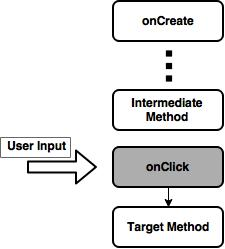
\includegraphics[scale=0.6]{DuplicationNStitching-1}\label{subfig:dup_stitch_1}}
% %  \subfloat[After Duplication and %Stitching]{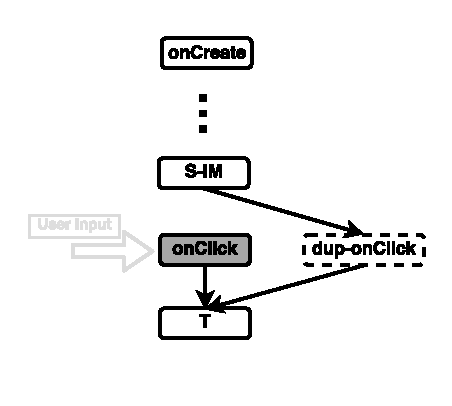
\includegraphics[scale=0.6]{DuplicationNStitching-2}\label{subfig:dup_stitch_2}}
% %  \label{fig:dup_stitch}
% %  \caption{Original app's flow Vs Modified app's flow}
% %\end{figure*}

% In order to do so, ordinary methods which are duplicates of the event listeners are created and instrumented inside in the app's smali files. Figure \ref{subfig:dup_stitch_1} shows a sample control flow of an application which starts at the \textit{onCreate} method and passes through some intermediate methods. At the \textit{onClick} method, it requires a UI event to proceed the execution along the target path. Dependability on the UI event (and for that matter on any system event too) is removed using a duplicate method of the event listener represented by dashed rectangle as shown in Figure \ref{subfig:dup_stitch_2}. So, these duplicate methods can be called to ensure stimulating the functionality coded inside the event listeners without providing any external events. The duplicate methods are named so that their names portray a relation between the duplicate method and the original event listener. Moreover, the system also keeps tracks of the duplicate methods so that an event listener is not duplicated more than once.

% %\todo[inline]{Need to design a naming convention for the duplicate methods so that they provide enough information about the original event listener.}

% \begin{figure}[t!]
% \centering
% \subfigure[Original]{
% \centering
% 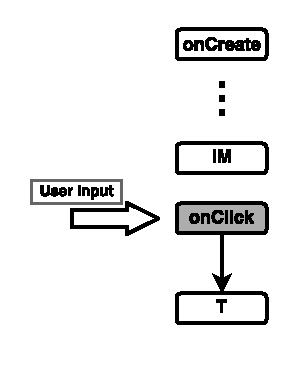
\includegraphics[scale=0.6]{DuplicationNStitching-1.pdf} %[width=.25\textwidth]
% \label{subfig:dup_stitch_1}
% }
% ~%Nothing
% \subfigure[Intrumented]{
% \centering
% 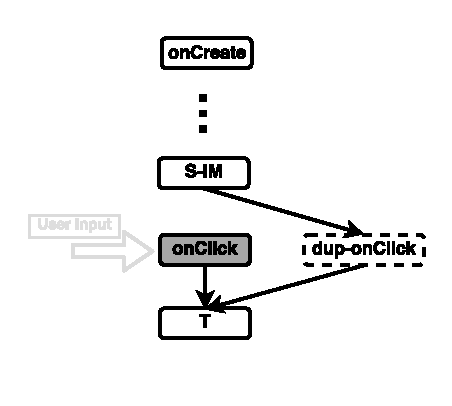
\includegraphics[scale=0.6]{DuplicationNStitching-2.pdf}
% \label{subfig:dup_stitch_2}
% }
% \caption{Original app's flow Vs Instrumented app's flow}
% \label{fig:dup_stitch}
% \end{figure}

% \subsection{Stitching: Inter-Method Control Flow}

% The control flow of an application from its entry point towards a given target is not always spontaneous, but it has to go through a number of user and system events at appropriate positions. Therefore, the extracted slice misses connectivity where the next method in the slice is an event listener. The connectivity at these critical points is dependent upon the UI/system events corresponding to the event listener. In order to remove this dependency, we connect the (duplicates of) event listeners to their preceding methods in the control flow and we call this process \textit{Stitching}. The stitching process consists of insertion of an direct method call to the (duplicate) event listener method in the method which precedes it according to the information provided by the extracted code slice in the first step.

% \begin{lstlisting}[language=java, label={lst:stitching}, caption={Stitching the Duplicate Methods}]
% ...
% //Inserted Method call
% invoke-virtual {p0, v0}, Ldisi/unitn/targettriger/testapp/MainActivity;->duplicate-onClick()V
% ...
% \end{lstlisting}

% Listing \ref{lst:stitching} shows an example of such an inserted method call. Location of the stitches depends upon the position of the event listener in the slice. Event listeners at the start of a slice (event listener as an entry point of the slice) would require their duplicate methods to be stitched with the \textit{onCreate} in MainActivity of the app. Also, there can be cases where all the statements that form a slice are from a single event listener. Such cases are handled similarly. However, when there is an event listener in the middle or at the end of the slice, a stitch needs to be placed in the method immediatedly preceding the event listener in the slice. Stitching ensures that the functionality coded insided an event listener is executed without the occurence of the required event as shown in Figure \ref{subfig:dup_stitch_2}.




% \subsection{Ensuring Intra-Method Control Flow}

% %Note: Remember Opaque predicates
% %We don't need to go for Opaque predicates, rather we follow the path in the code slice.


% Stitching accounts for the inter-method flow of the app execution. However, the intra-method flow an app execution might be hindered by the app's logic itself, such as the presence of conditional statements. TExeDroid traverses each method in the slice and extracts information on whether and how a conditional statement might affect the target. For instance, a conditional statement might be irrelevant to the target statement or it's \texttt{if}/\texttt{else}/both clause might have an effect on the target statement. In case, where the target statement depends upon the \texttt{if} clause only, the triggering system instrument the conditional statement to be always true, and vice versa. However, when execution of both the \texttt{if} and \texttt{else} clauses might affect the target statement, our system deals them in two separate runs of execution, one each for the \texttt{if} and \texttt{else} clause. Listings \ref{lst:conditional_statement} the instrumentation performed for the above mentioned cases.

% \noindent\begin{minipage}{.25\textwidth}
% \begin{lstlisting}[language=java, caption={\texttt{if} clause},label={lst:if}]
% ...
% if(true){
% 	//if clause
% }
% else{
% 	//else clause
% }
% ...

% TARGET.call();
% \end{lstlisting}
% \end{minipage}\hfill
% \begin{minipage}{.25\textwidth}
% \begin{lstlisting}[language=java, caption={\texttt{else} clause}, label={lst:else}]
% ...
% if(false){
% 	//if clause
% }
% else{
% 	//else clause
% }
% ...

% TARGET.call();
% \end{lstlisting}
% \end{minipage}





% However, the relation between the conditional statement and the actual statement can not always be that simple. In cases where there is no relation between the variable used in the conditional statement and those used in the actual statement, simply making the condition \texttt{true} works fine. However, if the variables in the conditional statement have a direct effect on the actual statement, the previous solution may or may not work, specially in cases where these values are taken from the outside world. In cases where the variable used in the condition is also used in the target statement, we instrument the conditional statement in three different ways, i.e., replacing the condition by a boolean \texttt{true}, \texttt{false} and change the value of the variable such that the condition becomes \texttt{true}. This instrumentation ensures the execution of the target statement, however, this still does not guarantee an accurate solution for the problem when the values of the variable used are taken from the outside world at runtime, such as through an SMS or from the Internet. For instance, a variable \textit{x} which takes its value from an incoming SMS and its value is zero/null otherwise. If there is a conditional statement such as \texttt{if(x)} followed by a target statement such as \texttt{sendTextMessage(x,..);}, we will never know the exact value of the \textit{x} and making it true doesn't solve the issue completely. However, cases where conditional statements are like \texttt{if(x==y)} are followed by the target statement can be solved, where \textit{y} is another variable/constant whose value is known. Similar reasoning applies to other conditional statements as well, such as \texttt{switch} statement.

% \todo[inline]{Basic block concept in the above para}
% \todo[inline]{Commenting invoke statements where the control diverts to non-relevant method.}

% \iffalse

% \subsection{Logging Critical Info}

% \textbf{General:} The purpose of dynamic analysis is to know the behavior of an app. Target-Trigger, however, focuses only on the execution of certain paths leading to specific APIs. In order to know the runtime values of the parameters passed to these target APIs, we instrument the app with hooks placed before every target API call. These hooks make sure to capture the runtime values of such parameters of interest.

% \textbf{StaDyna:} In case of coupling T-TDroid with StaDyna (a tool for resolving the targets of reflection and dynamic class loading) as a triggering solution, StaDyna requires additional information to identify the correct position of the called methods in the method call graph. Stadyna generates a complete method call graph of the application taking into consideration the runtime calls to reflection APIs and the code which is loaded dynamically. For generating a complete method call graph, it is important to know the exact position of new nodes that are to be added to the method call graph. This additional information is required only when the reflection/dynamic class loading calls are inside the duplicated event listeners. There, in order to capture this additional information, T-TDroid places hooks in the duplicated even listeners which provide information about their actual counterparts.
% \fi

% \subsection{Execution along the target path}

% Once the instrumentation related to a particular slice is over, TExeDroid reassembles the app from its Smali files and signs it. The repackaged app is then installed on a target device or emulator. The instrumentation explained in this section above makes sure that the application follows the target path (for a specific slice), once launched, without requiring any external UI or system event. Instrumentation is performed for a particular target (one target execution path at a time) and, hence, it must be repeated for each target in the app. Therefore, TExeDroid works in an instrument-repackage-launch cycle where the number of the instrument-repackage-launch cycles is less than or equal to the number of target statements in the app. In case an app having inline slices, multiple slices are triggered in the same instrument-repackage-launch cycle.



% %######################################################################################


% \iffalse

% We use a precise and efficient methodology for targeted test case generation.

% \begin{itemize}
% \item Method Call Graph generation
% \item Target paths extraction
% \item Node categorization in the target paths (Callback methods, UI events, System events, other methods)
% \item Symbolic execution of methods where necessary
% \item Use the above info generating an accurate chain of actions (test cases) which leads to target in the give app
% \end{itemize}

% We use symbolic execution for targeted test case generation. Symbolic execution usually suffers from the path explosion problem. It is an expensive method of test case generation and takes a lot of time. To cater these problems, our symbolic execution engine is based on a Method Call Graph (MCG) of the application. The MCG is used to guide the symbolic execution engine and prune unnecessary exploration. A coarse view of the whole process is show in Figure \ref{fig:work_flow}.

% \begin{figure}[h]
% \centering
% 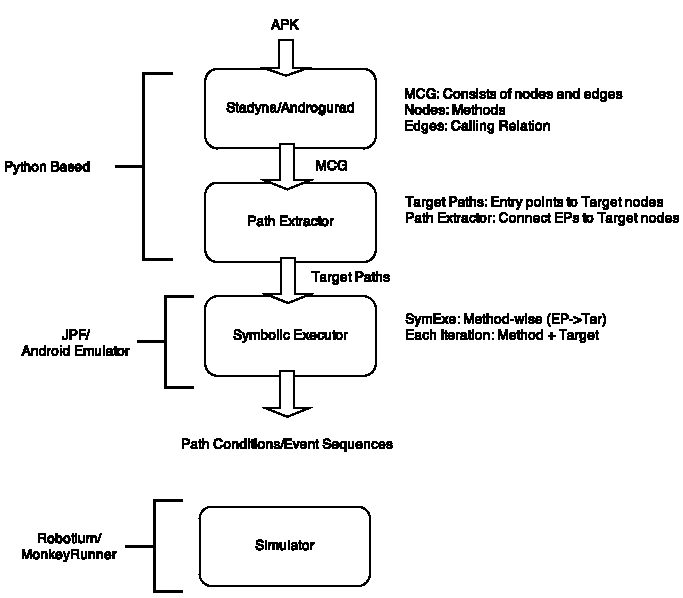
\includegraphics[width=14cm]{TTeCGAT-Workflow}
% \caption{TTeCGAT Work Flow}
% \label{fig:work_flow}%
% \end{figure}

% \subsection{Stitched Method Call Graph}

% An MCG consists of nodes and edges where nodes represent methods and edges represent a calling relation between the methods. The MCG is constructed from the Dalvik bytecode of the application. Android apps are mostly event (both user and system) driven and contain callback methods of the framework which are implemented by the app developer. Generally, the flow of an app may vary from one execution to another based on the received user and system events. Moreover, Android app components such as activities and services are started using intent messages rather than a direct method call. Therefore, a statically generated MCG consists of several disconnected MCGs. These disconnected MCGs need to be stitched together, based on sources of targets of intent messages, to form a Stitched Method Call Graph.

% The nodes in the MCG are divided into three categories. 1) Entry point (EP) 2) Intermediate nodes 3) Target nodes. EPs correspond to the methods from where an application can be stimulated. Target nodes represent those methods which contain the target code (line, API, method, etc.) for which we want to generate test cases. Intermediate nodes are those methods which construct the path from EPs to target nodes.


% \subsection{Extraction of Target Paths: Reducing the search space}

% After construction of the MCG and identification of the EPs and target nodes, the next step to extract the paths, which start from the EPs and lead to the target node through one or more intermediate nodes. Sometimes, the EP may directly be connected to the target node without having any intermediate nodes in between. Moreover, a node can be an EP as well as a target node at the same time. Target paths are extracted from the MCG by traversing it from a target node in backward until an EP is reached. There can be cases where more than one target paths, starting from the same or different EPs, are extracted for the same target. Moreover, a non-deterministic interleaving of callback methods based on user and system events makes it harder to find out the exact flow of events which lead to a certain target node. In addition, there may be methods which may not be part of the original path which leads to the target node, but effect the state of app in such a manner that is essential for reaching the target node. So, it is important to include these supportive methods in the search space. Here, the search space is essentially reduced using the MCG.

% \subsection{Symbolic Execution}

% Our Symbolic execution engine is guided by the extracted target paths. We perform a two-level symbolic execution of the app. 1) A method-wise symbolic execution for all the nodes in the target path. The aim of the symbolic execution is to generate test cases for each method which can lead to the next method on the specific target path. So, each node has a method name and target inside that method for which symbolic execution engine tries to generate test cases. The test cases generated for one method are fed to the symbolic execution engine of the next method which has a newer target corresponding to the next method in the target path. 2) The second level of symbolic execution tries to find out the combination of these methods which lead to the target node. So, at the stage a more concise list of methods is identified which helps in generating a possible test case for the app. This process continues until a possible test case (a sequence of events) is generated which can stimulate the application from an EP to the target. This process is repeated for all the target paths (paths from EPs to targets).

% \subsection{Stimulating Applications}

% At end of the symbolic execution process, we get one or more test cases for each target path, which are converted to concrete event sequences. These event sequences are then fed to a simulator (such as Robotium, MonkeyRunner, etc.) which exercises the original application on an Android emulator or real device.

% \fi

\section{Fingerprints}
\label{sec:implementation}
As discussed before, in this work usage-profile statistics were collected by running  Java code only, since the most sandbox are not able to analyze the native code behaviors we intentionally choose to avoid native code in our scouting application. Collecting data in Android is easy as call the specific exposed Android API. We released our scouting application as open-source project, it is published at the following address \footnote{\url{https://vaioco.github.io/avfingerprint}}.
The scouting application requests in its AndroidManifest all possible Android permissions to maximize its capabilities within confinement of the application sandbox. \\
In the following subsections, we present the details of collected data.

\subsection{Environment artifact}
The scouting application collects its environment data exploiting the Android API, which are basically wrappers to the underlining system services. We collected data from only a specific domain: environment-based data. \\  
Differently from previous works \cite{petsas2014rage}\cite{vidas2014evading}\cite{jing2014morpheus} where performance , low level discrepancy, system property data are collected to detect Android emulators, we used a totally different approach. Instead of looking for discrepancy in the runtime behavior or scanning the file system looking for well known files, we do something innovative collecting and analyzing the environment data. \\
Here we define an interesting \textit{environment artifact} as artifact whose presence can be probed or whose contents can be read by any Android application in its sandbox using only Java code.
The main idea of this work is that environment artifact should look like user-generated data, otherwise malicious applications could use a fingerprint-based approach to detect and then evade the sandbox analysis. \\
An \textit{environment artifact} is by definition related to the running environment, it is not related to specific system properties, like kernel objects exposed by the pseudo file systems or the Android property system. Such artifact should be created by the user who own the devices which is running the application.
In the following we detail the type of collected data shown in Table \ref{tab:data}

\begin{itemize}
\item Contacts: Requiring the specific permission an application can easily query the \textit{ContactProvider} to get the contact list from the device. The scouting application does a query to get out all the available information from the \textit{ContactsContract.Data} table for each contact.
\item SMS: Stored by a content provider, requiring the specific permission an application can list SMS from inbox, sent and draft container. The scouting application collects all stored SMS along with all information, specified by interface \textit{Telephony.TextBasedSmsColumns}, stored in the content provider.
\item Calls: Information about placed, received and recents calls is stored by the \textit{android.provider.CallLog} provider. Our scouting app retrieves all calls' information as detailed by the class \textit{android.provider.CallLog.Calls}.
\item Location: Android offers several location strategies \footnote{\url{https://developer.android.com/guide/topics/location/strategies.html}} like the GPS and Android's Network Location Provider to acquire the user location. Although GPS is most accurate, it only works outdoors. Android's Network Location Provider determines user location using cell tower and Wi-Fi signals, providing location information in a way that works indoors and outdoors. We used both strategies to get the location and sent it back to the remote server.
\item Battery: Android provides the \textit{BatteryManager} API to retrieve the battery status\footnote{\url{https://developer.android.com/training/monitoring-device-state/battery-monitoring.html}}. Monitoring the battery information \footnote{\url{https://developer.android.com/training/monitoring-device-state/battery-monitoring.html}}  permits to determine the current charging state, the battery level and monitor when the device is connected and disconnected from power.
\item Wi-Fi: The \textit{WifiManager} class provides the primary API for managing all aspects of Wi-Fi connectivity. It permits to collect several categories of items:
\begin{itemize}
\item The list of configured networks.
\item The currently active Wi-Fi network, if any.
\item Results of access point scans.
\end{itemize}
\item Applications: The class \textit{android.content.pm.PackageManager} permits to get various type of information related to the application packages that are currently installed on the device. This information is strongly related to the running environment, in fact the Android emulator contains a fixed set of installed applications. 
\end{itemize}
\section{Evaluation and Discussion}
\label{sec:discussion}
This section presents experimental results that characterize the effectiveness of TeICC to analyze apps that conceal sensitive information flow using obfuscated ICC.
We evaluate TeICC on two benchmark test suites, DroidBench~\cite{droidbenchpage} and ICC-Bench~\cite{wei2014amandroid}, specifically crafted for testing tools to detect information flow concealed using ICC. ICC-Bench includes 9 test case apps
and DroidBench contains 23 apps included in the \emph{InterComponentCommunication} test case. The goal of evaluation of TeICC is to test its capability to extract slices across multiple components in obfuscated apps and execute them. Therefore, we obfuscated these ICC-based test suites using DexGuard\cite{dexguardpage} to evaluate TeICC.

%We use ICC-Bench and DroidBench test suites for comparison purpose  because they consist of apps designed to specifically test ICC mechanism and we use them as \emph{ground truth} because for those apps all ICC flows are known in advance.

%We want to note that TOOLNAME is not intended for finding suspicious leakage across different Android components.

%Although,
%our backward-slicing approach is generic and can be used for any data-flow analysis, we focus in this paper on: extraction of slices across different components from an obfuscated app and then execute them on a real world device. 

% Additionally,  we evaluate TOOLNAME on two different sets, the former composed by 100 apps crawled from the GooglePlay\cite{GooglePlay_webpage} store by retrieving the top 100 free apps. The latter contains 100 randomly selected malware from the IccTA dataset\cite{iccre}, it includes malware apps which use ICC flows to exchange sensitive data.

Table \ref{tab:droidbench} shows evaluation results for both DroidBench and ICC-Bench test suites. For brevity we group the apps in categories. The second column contains the number of ICC links found by TeICC while the third and fourth column show if the apps have been correctly analyzed by IccTA\cite{li2015iccta} and TeICC, respectively. The symbol \ding{56} means that the tool has failed to analyze the app and the symbol \ding{52} means that the app has been properly analyzed. Not surprisingly, TeICC outperforms IccTA on both tests since IccTA cannot detect ICC methods called by Java reflection and encrypted strings used in intents. As shown in Table~\ref{tab:droidbench}, TeICC can automatically extract-then-execute 100\% of ICC flows in all apps; except for those which perform ICC involving a \emph{Content Provider} because currently TeICC does not provide support for Content Providers. Unfortunately, we cannot evaluate Harvester\cite{rasthofer2016harvesting} because it is not open source. However, we understand that it will not be successful as well because it does not support slicing across different Android components.


\renewcommand{\arraystretch}{1.2}


\iffalse
\begin{table*}[!htbp]
\centering
\begin{tabular}{@{}cccccccc@{}} \toprule
\multicolumn{8}{c}{Destination Component} \\ \cmidrule(l){2-8}
& & Activity & Service & Provider & Receiver & Sum & Triggered \\ \midrule
\multirow{3}{*}{Source Comp.} & Activity & 41115 & 7696 & 0 & 31147 & asd & asd \\ 
& Service & 45890 & 9080 & 0 & 36233 & asd & asd \\ 
%& Provider & 0 & 0 & 0 & 0 & asd & asd \\
& Receiver & 2021 & 390 & 0 & 1605 & asd & asd \\ 
\bottomrule
\end{tabular}
\caption{Malware apps}
\label{tab:mlw}
\end{table*}
\fi
\iffalse
\begin{table*}[!htbp]
\centering
\begin{tabular}{@{}cccccccc@{}} \toprule
\multicolumn{8}{c}{Destination Component} \\ \cmidrule(l){2-8}
& & Activity & Service & Provider & Receiver & Sum & Triggered \\ \midrule
\multirow{3}{*}{Source Comp.} & Activity & 36239 & 4114 & 0 & 55926 & asd & asd \\ 
& Service & 0 & 184 & 0 & 0 & asd & asd \\ 
%& Provider & 0 & 0 & 0 & 0 & asd & asd \\
& Receiver & 4057 & 454 & 0 & 6275 & asd & asd \\ 
\bottomrule
\end{tabular}
\caption{GooglePlay store apps}
\label{tab:normal}
\end{table*}
\fi
\iffalse
\begin{table*}[!htbp]
\centering
\begin{tabular}{@{}cccccccc@{}} \toprule
\multicolumn{8}{c}{Destination Component} \\ \cmidrule(l){2-8}
& & Activity & Service & Provider & Receiver & Sum & Triggered \\ \midrule
\multirow{3}{*}{Source Comp.} & Activity & 240 & 0 & 0 & 7 & asd & asd \\ 
& Service & 0 & 1 & 0 & 0 & asd & asd \\ 
%& Provider & 0 & 0 & 0 & 0 & asd & asd \\
& Receiver & 34 & 0 & 0 & 1 & asd & asd \\ 
\bottomrule
\end{tabular}
\caption{DroidBench apps}
\label{tab:droidbench}
\end{table*}
\fi

\begin{table}[!htbp]
\centering
\begin{tabular}{@{}cccc@{}} \toprule
Apps & ICC & IccTa & TeICC \\ \midrule
%\cmidrule(l){1-4}
\multicolumn{4}{c}{DroidBench} \\ \cmidrule(l){1-4}
startActivity[1-7] & 2/9 & \ding{56} & \ding{52}  \\
startActivityForResult[1-4] & 0/8 & \ding{56} & \ding{52}  \\
sendBroadCast1 & 0/1 & \ding{56} & \ding{52} \\
sendStickyBroadCast1 & 0/1 & \ding{56} & \ding{52}  \\
startService[1-2] & 0/2 & \ding{56} & \ding{52} \\
bindService[1-4] & 0/4 & \ding{56} & \ding{52} \\
ContentProvider[1-4] & 4/0 & \ding{56} & \ding{56} \\
%query1 & 1/0 & \ding{56} & \ding{56} \\
%delete1 & 1/0 & \ding{56} & \ding{56}  \\
%insert1 & 1/0 & \ding{56} & \ding{56}  \\
%update1 & 1/0 & \ding{56} & \ding{56}  \\
\cmidrule(l){1-4}
\multicolumn{4}{c}{ICC-Bench} \\ \cmidrule(l){1-4}
Explicit1 & 0/1 & \ding{56} & \ding{52} \\
Implicit[1-6] & 7/0 & \ding{56} & \ding{52} \\
DynRegister[1-2] & 2/0 & \ding{56} & \ding{52} \\
\bottomrule
\end{tabular}
\caption{DroidBench/ICC-Bench apps.  ICC: \# of implicit/explicit transitions between components.}
\label{tab:droidbench}
\end{table}
 
 
%\begin{itemize}
Our results indicate that TeICC permits to effectively extract-then-execute the target slices obtained from the program slicing analysis. If, for instance, the target app contains checks which could prevent the dynamic analysis (\textit{i.e.,} emulation detection, integrity checks, etc.), they are not extracted in the slicing step (unless they hold a data dependence with the MOI). 
%\item 
%TOOLNAME has different features over the current state of the art of both dynamic and static analyzer. 
In contrast to Harvester \cite{rasthofer2016harvesting}, TeICC supports the ICC mechanism which enables it to automatically extract-and-execute target slices that belong to  different Android components. Similarly, R-Droid \cite{backes2016r} lacks support for both ICC and Java reflection mechanisms.  
Compared to IccTa\cite{li2015iccta},
TeICC, based on a hybrid approach, permits to enrich the original app after its targeted execution to resolve obfuscated parts of the app. Over different executions it permits to extract runtime values from reflection calls or dynamically loaded code and integrate them in the analysis for the next iteration. 
%\end{itemize}

At the moment TeICC does not support the \emph{Content Provider} component; we leave it as future work. Moreover, it does not analyze native code. For instance, if an SMS message is sent from native code, TeICC cannot use this hidden call to \emph{sentTextMessage()} as MOI. However, just like TeICC, both \cite{rasthofer2016harvesting} and \cite{backes2016r} also do not support native code analysis.



% \begin{tikzpicture}
% \begin{axis}[
%     ybar stacked,
%     enlargelimits=0.15,
%     legend style={at={(0.5,-0.20)},
%       anchor=north,legend columns=-1},
%     ylabel={\#participants},
%     symbolic x coords={tool1, tool2, tool3, tool4, 
% 		tool5, tool6, tool7},
%     xtick=data,
%     x tick label style={rotate=45,anchor=east},
%     ]
% \addplot+[ybar] plot coordinates {(tool1,0) (tool2,2) 
%   (tool3,2) (tool4,3) (tool5,0) (tool6,2) (tool7,0)};
% \addplot+[ybar] plot coordinates {(tool1,0) (tool2,0) 
%   (tool3,0) (tool4,3) (tool5,1) (tool6,1) (tool7,0)};
% \addplot+[ybar] plot coordinates {(tool1,6) (tool2,6)
%   (tool3,8) (tool4,2) (tool5,6) (tool6,5) (tool7,6)};
% \addplot+[ybar] plot coordinates {(tool1,4) (tool2,2) 
%   (tool3,0) (tool4,2) (tool5,3) (tool6,2) (tool7,4)};
% \legend{never, rarely, sometimes, often}
% \end{axis}
% \end{tikzpicture}

% \begin{table}
% \centering
% \caption{ICC-dataset}
% \begin{tabular}{|c|c|c|} \hline
% Type&Type&Results\\ \hline
% \multirow{4}{*}{Components} & Activity  & 1229 \\ 
% & Service  & 72 \\ 
% & Receiver & 6 \\ 
% & Provider & 152 \\  
% \hline
% \multirow{6}{*}{Intents} & Implicit & asd \\
% & Explicit & asd \\ 
% & Activity & 1412 \\
% & Service & 90 \\
% & Receiver & 0 \\
% & Provider & 34 \\ 
% \hline
% \multirow{4}{*}{ExitPoints} & Activity & 1453 \\
% & Service  & 111 \\ 
% & Receiver & 152 \\ 
% & Provider & 36 \\ 
% \hline
% \end{tabular}
% \label{tab:sandbox}
% \end{table}

%---------------------------------------------
%DroidBench Analysis
\iffalse
1. ActivityCommunication1
 - Activities : 2
 - No direct link between the activities (taskAffinity - have to check)
 - DataFlow : Activity2.onCreate: source -> Activity1.data1; Activity1.onCreate: data1 -> sink
 
2. ActivityCommunication2
 - Activities : 3
 - One link from OutFlowActivity -> InflowActivity. StartActivity using Intent declared in the manifest manipulated using substring(). 
 - DataFlow: OutFlowActivity gets data and starts InflowActivity which leaks it.

3. ActivityCommunication3
 - Activities : 3
 - 1 link : Activity resolution activity.getClassName()
 - DataFlow : OutFlowActivity gets data and starts InflowActivity which leaks it.
 
4. ActivityCommunication4
 - Activities : 3
 - One link from OutFlowActivity -> InflowActivity. StartActivity using Intent declared in the manifest manipulated using string concatenation. 
 - DataFlow: OutFlowActivity gets data and starts InflowActivity which leaks it.
 
5. ActivityCommunication5
 - Activities : 3
 - One link from OutFlowActivity -> InflowActivity. StartActivity using ComponentName object by providing the name of InFlowActivity. 
 - DataFlow: OutFlowActivity gets data and starts InflowActivity which leaks it.
 
6. ActivityCommunication6
 - Activities : 3
 - One link from OutFlowActivity -> InflowActivity. StartActivity using using Intent passed through a List object of intents. 
 - DataFlow: OutFlowActivity gets data and starts InflowActivity which leaks it.
 
7. ActivityCommunication7
 - Activites : 3
 - One link from OutFlowActivity -> InflowActivity. StartActivity using using Intent with non-constant Activity.getClass(). 
 - DataFlow: OutFlowActivity gets data and starts InflowActivity which leaks it.
 
8. ActivityCommunication8
 - Activities : 3
 - One link from OutFlowActivity -> InflowActivity. StartActivity using using Intent where the action string is passed to the Intent through a List object of Strings. 
 - DataFlow: OutFlowActivity gets data and starts InflowActivity which leaks it.
 
9. BroadCastTaintAndLeak1
 - Activities : 1
 - Receivers : 1 (Declared and registered inside the Activity)
 - OnCreate registers a receiver which leaks data which is provided by onDestroy of the Activity.
 
10. ComponentNotInManifest1
 - Activities : 2 (2 more which are not declared in the manifest)
 - Links : No link, apparently OutFlowActivity gets IMEI, calls startActivity for InFlowActivity, but since InFlowActivity is not declared in the manifest, it won't start. InFlowActivity does contain the code for leaking IMEI.
 
11. EventOrdering1
 - Activities : 3
 - Links : OutFlowActivity activity start InFlowActivity. 
 - DataFlow : InFlowAcitivty has a method which reads IMEI and writes it to sharedPref. If this activity is called by some foreign app before its being called by OutFlowActivity, it will read IMEI and write it sharedPref. Then, when OutFlowActivity calls it, it leaks the IMEI. Otherwise NOT. In our case, we will extract the slice, execute it, but it won't leak IMEI.
 
12. IntentSink1
 - Activities : 1
 - Activity gets IMEI and writes it to an Intent which is added to the .setResult() of the activity. The Intent will be received by the calling activity and so as the IMEI. 
 
13. IntentSink2
 - Activities : 1
 - Activity reads IMEI, reads an appName provided by the user via an EditText field and starts the appName with an Intent containing the IMEI.
 
14. IntentSource1
 - Activities : 1
 - DataFlow : From onCreate to onActivityResult of the same activity. In the onCreate, the activity starts the same activity by calling startActivtyForResult. 
 
15. ServiceCommunication1
 - Activities : 1
 - Services : 1
 - ICC Link : Activity -> Service
 - DataFlow : Activity reads IMEI after a user presses a button and sends it to the Service using Binder messaging service.
 
16. SharedPreferences1
 - Activities : 2
 - MainActivity reads IMEI, writes it to sharedPref. OtherActivity reads sharedPref and leaks it. 
 - Links : No direct link between the activities (like start activity or something)
 
17. Singleton1
 - Activities : 2
 - MainActivity onCreate write "" to a string in a Static Class Singleton's field s. It onStop leaks it. OtheActivity writes IMEI to the same field. It otherActivity gets executed before MainActivity, leakage will take place. Otherwise NOT.
 
18. UnresolvableIntent1
 - Activities : 3
 - Links : 2, OutFlowActivity calls either InFlowActivity1 or InFlowActivity2 based on a random number generator. 
 - DataFlow : OutFlowActivity -> InFlowActivity and OutFlowActivity -> InFlowActivity2
\fi
%----------------------------------------------



\section{Chapter Summary}
\label{sec:conclusion}
In this chapter, we presented a targeted triggering approach, TeICC, to stimulate ICC in Android apps. TeICC is based on backward program slicing which in turn relies on a SDG. The SDG based backward slice extraction technique used by TeICC enables it to extract-then-execute target slices across multiple app components. Moreover, the iterative hybrid approach allows TeICC to extract runtime values (\textit{i.e.,} reflection values, decrypted strings, etc.) to enrich the original app. These runtime values help in performing improved static analysis of obfuscated apps in the next iteration. 

As a future work, we would like to provide support for content providers. Moreover, we focus on different approaches to overcome current limitations. For example, to address the extraction of slices involving native calls, we are analyzing a novel approach using the ARTDroid \cite{costamagnaartdroid} framework to intercept sensitive Java methods called by native code.

\chapter{StaDART: Combining Static and Dynamic Analysis}
In this chapter, we present StaDART, an extented version of our previously proposed solution Stadyna, which combines static and dynamic analysis of Android applications to reveal the concealed behavior of malware. Unlike Stadyna, StaDART utilizes ArtDroid to avoid modifications to the Android framework. Furthermore, we integrate it with a triggering solution, DroidBot, to make it more scal- able and evaluate it with more Android applications. We present our evaluation results with a dataset of 2,000 real world applications; containing 1,000 legitimate applications and 1,000 malware samples.



\section{Introduction}

Ensuring smartphone users' privacy and security is a major concern and requires adequate measures from app developers, framework providers, and app stores, etc. Google's open source operating system, Android, being the most popular platform for mobile devices, uses Google Bouncer as an app vetting process at its official Google Play store. Vetting processes generally use some form of static/dynamic analysis to scrutinize apps for malicious content and Google Bouncer is no different. In addition, starting from Android 7.0, Android introduced Verify Apps, a new security feature to analyze apps downloaded from sources other than the Google Play store. 

%~\cite{google-bouncer}

However, a growing number of malware samples found in the Android ecosystem reveals that malware developers bypass such vetting processes using various evasion techniques. Previous research shows that the use of dynamic code update techniques along with various forms of obfuscation makes it extremely hard for the state-of-the-art analysis tools to understand the behavior of an app\cite{ExecuteThis_Poeplau2014, ahmad2016empirical}. Thus, the use of these evasion techniques in newly found malware is not surprising~\cite{brain-test}. This paper provides an empirical demonstration of the lack of effectiveness of the state-of-the-art tools when it comes to analysing apps that hide suspicious behavior using reflection and dynamic code loading. We develop a set of benchmark apps that use reflection in different ways to conceal information leakage. Our analysis of reflection-bench using some of the state-of-the-art static analysis tools shows their ineffectiveness to handle apps that use reflection. Furthermore, we develop InboxArchiver, a seemingly benign app that uses dynamic code loading to hide its suspicious functionality, and use it to test some of the most well known online analysis services. The analysis show that InboxArchiver easily bypasses these security analysis services. %\footnote{Similar proof of concept apps, which were able to 

Static analysis relies on the availability of all the information at analysis time, hence, it suffers  from dynamic features and unavailability of information that are known only at execution time, e.g., the parameters used in the dynamic code update APIs. Therefore, reflection that is a programming technique widely used by mobile app developers can be only partially investigated by current  static analysis tools. As a result, reflection is usually used by malware developers to hide malicious code. The inherent limitation of  all static analyzers  (e.g., \cite{FlowDroid_Arzt2014,Saaf_Hoffmann2013}) is the operational assumption  that the code base does not change dynamically and the targets of reflection calls can be discovered in advance. This is a clear simplification of what happens in the real world, where many apps rely on code base updates instantiated only at runtime.


There exist approaches that enhanced static analyzers of Java code to deal with the presence of dynamic code update techniques (e.g., \cite{TamingReflection_Bodden2011}). However, they cannot be  applied directly to Android due to the differences in the Java and Android platforms. The alternative of instrumenting the app offline has the  major drawback of breaking the app signature, that some apps check  at runtime. As the app starts, it checks the integrity of the signature against  a  value hardcoded in the app and terminates if the check fails. In case of malicious apps this check may be used to conceal illicit behavior. 

In this paper, we present StaDART, a mobile app security analysis tool that combines static and dynamic analysis to address the presence of dynamic code updates. Instead of relying on modifications to the Android framework, StaDART utilizes a vtable tampering technique for API hooking to perform dynamic instrumentation~\cite{costamagna2016artdroid}. Furthermore, we integrate StaDART with DroidBot, a triggering tool for Android apps, to make the analysis  fully automated. StaDART is evaluated using a dataset of 2,000 real world apps (both malicious and benign) and the results of our evaluation reveal that it is more common in malicious apps to use dynamic code updates to conceal malicious behavior which is only exhibited once the app is installed on a real device. Moreover, 33\% of malware samples that use DCL introduce APIs guarded with new (not used in the initial code base) dangerous permissions in the newly loaded code, whereas the analysed benign apps do not exhibit such behavior.  

\textbf{Contributions:}

\begin{itemize}
\item We present the design and implementation of StaDART, a system that interleaves static and dynamic analysis in order to reveal the hidden/updated behavior of Android apps. By utilizing vtable tampering for API hooking, we avoid modifications to the Android framework and make it largely framework independent. StaDART analyzes the code loaded dynamically, and is able to resolve the targets of reflective calls complementing app's method call graph with the obtained information. Therefore, StaDART can be used in conjunction with other static analyzers to make their analysis more accurate.

\item We integrate StaDART with DroidBot to make it fully automated and to ease the evaluation. Moreover, we analyze a dataset of 2,000 real world apps (1,000 benign and 1,000 malicious). Our analysis results show the effectiveness of StaDART in revealing behavior which is otherwise hidden to static analysis tools.  

\item We release our tool as open-source to drive the research on app analysis in the presence of dynamic code updates.
%\footnote{\url{new link}}
\item We design and develop reflection-bench, a set of benchmark apps that use reflection to conceal information leakage, and use it to test some of the state-of-the-art static analysis tools. We publish reflection-bench so that researchers can test the effectiveness of their analysis tools in the presence of dynamic features (i.e., reflection). 

\end{itemize}

\textbf{Paper Organization:}

\S\ref{sec:info_android} provides a background on dynamic class loading and reflection in Android. 
\S\ref{sec:refbench_dcl} discusses the design and implementation details of reflection-bench and InboxArchiver. It also provides the analysis results highlighting the shortcomings of state-of-the-art Android app analysis tools. \S\ref{sec::system_general_description} gives a high-level description of StaDART, while \S\ref{sec::implementation} covers the implementation details. \S \ref{sec:mcg_description} presents our approach to build method call graphs and visualise them. \S\ref{sec:evaluation} reports the evaluation results of StaDART on real world apps. \S\ref{sec:discussion} discusses the limitations of the current implementation, and envisages the future work. \S\ref{sec:relwork} overviews the related work, and \S\ref{sec:conclusion} concludes the paper.


\section{Application Scenario} \label{sec:app-scenario}

In this section, we provide a motivating example to highlight the advantages of our approach. The example refers to the enterprise domain where services like MAMs and MDMs are usually deployed to manage devices and apps used by employees.  \\

Here we stress that \asd's main goal is to be able to enforce security-and-privacy policies for customising the behaviour of  apps without modifying their code. 
\asd is not a mobile malware detector. Anti-malware solutions are complementary to \asd. \asd is an enterprise tool used to customise the security policy of the mobile applications employees run.
Such customisations are required because the enterprise may need to monitor and possibly restrict the benign app behaviour or the use of some features of the app, due to local legislation (e.g., privacy-related regulations) and/or enterprise security policies (e.g., banning the use of WiFi in particular contexts). 

\iffalse
\begin{figure*}[b]
\centering
\subfigure[app distribution model]{
\centering
\includegraphics[width=.35\textwidth, keepaspectratio, resolution=600]{1}
\label{fig:before}
}
~%Nothing
\subfigure[\asd distribution model]{
\centering
\includegraphics[width=.35\textwidth, keepaspectratio, resolution=600]{system_model_after}
\label{fig:after}
}
\caption{App distribution: (a) default scenario , (b) \asd in place}
\label{fig:appdistribution}
\end{figure*}
\fi

The scenario involves the following parties: (i) a developer $Dev$ and (ii) an enterprise $Ent$.
Let us assume that $Dev$ has created an app $A$ that $Ent$ wants to use. 
To wrap an app with a traditional MAM service, one has to have access to the source code of the app or the developer needs to apply the sandbox while developing her own app.
Unfortunately, $Ent$ \textbf{does not} have the source code of $A$, that could be heavily obfuscated, and $Dev$ does not want to release the source due to IPR reasons. $Dev$ is also not interested in customising $A$ using a wrapper $sandbox$  because of the extra resources needed for managing the customised version of $A$ and the cost of supporting further updates. 

\textbf{\asd.} In such a scenario, our approach can be useful. We envision the developer's cooperation to offer a \asd compatible version of $A$. 
However, $Dev$ does not need to branch any new version of $A$ or to include third-party library/code within the app. The only action needed is to run $A$ through our \stubMaker (more details will be provided in Section \ref{sec:stubfactory}).  This component takes $A$ as input and returns two apps: the \stub $A'_{stub}$  and $A'$. The $A'_{stub}$ will generate the sandbox where $A'$ will be executed (details will be discussed in Section \ref{sec:stub}). Here we stress that $A'$ is an exact copy of $A$ except for a slightly different manifest file automatically modified by the \stubMaker component. Moreover, it is important to note that \stubMaker neither  modifies $A$'s bytecode nor inserts any additional code in the app. The \stubMaker can take as input also the obfuscated version of $A$. 

At this stage, $Dev$ has to sign $A'_{stub}$ and $A'$ by a fresh generated self-signed certificate $K$. Finally, the signed new apps can be distributed so that \textit{Ent}, which owns the right for the certificate $K$, is able to retrieve it. 

When $Dev$ releases a new version of $A$, the only step required is to create a new version of $A'$. This process is fully automated by means of  \stubMaker which produces the new version of $A'$. Each time $Dev$ releases a new app's update she goes through this automated procedure in order to create the \asd compatible app, but differently from the first release there is no need to update and distribute $A'_{stub}$ again, because the stub code does not change upon to app's update. Finally, $Dev$ signs the new version of $A'$ with the digital certificate that has been used to sign the previous version of the app. 

\asd allows $Ent$ to monitor and possibly restrict the behaviour of $A'$. The specification of what to monitor, how and what to enforce can be done by $Ent$ by writing behavioral policies for \asd. Fine grained policy capability offered by \asd 
become even more relevant in scenarios such those depicted by the recently introduced European regulation, the General Data Protection Regulation (GDPR) \cite{gdpr}. In the following, we provide two examples of such policies: 

\begin{itemize}
\item Default enterprise security and privacy policies. This set of policies must be enforced on any app the employee installs on her phone. These policies enforce corporate-related data (i.e., contacts, calendar), copy/paste protection, corporate authentication, app-level VPN, data wipe and run-time integrity check, no HTTP connections.

\item Access restrictions to selected system resources. In some locations or in some circumstances (e.g., meeting) apps may be prevented access to some system features of the phone (e.g.,, alarm, wifi connectivity, camera, mic, etc.) 

\end{itemize}
We will show later in the paper how, in detail,  \asd  expresses and  implements such policies.

\section{Requirements}
In this section, we present the set of requirements that have driven the design of \asd. 

Our aim is to provide a lightweight app-level sandboxing solution for stock Android that does not require modifications of the apps' code. The following requirements are needed and are met by \asd:
\begin{itemize}
\item \textbf{R1:} No OS modifications and no root privileges. The mechanism must not require  modifications/extensions to the Android OS. Moreover, the mechanism must be able to operate without root privileges. 

\item \textbf{R2:} Permissions: The mechanism should not require more privileges and permissions than those originally requested by the app that will be sandboxed. 

\item \textbf{R3:} Universal: The mechanism can be applied to monitor and enforce policy on any app running on current and/or any previous version of Android, without requiring any app code modification or integration with SDKs.

\item \textbf{R4:} Java and native: The mechanism must support the monitoring and enforcement of policies, covering the app behaviour that can be captured at both Java and at native level.

\item \textbf{R5:} Lightweight: lower overhead when compared to existing solutions providing similar security features.
\end{itemize}

The first requirement, $R1$ is quite important especially when it comes to enterprise environments. Enterprises are not keen to deploy approaches that require root permissions or extensive modifications to the OS core components. In the former case, enabling root permissions might void the device's manufacturer guarantees and open the door to  critical attacks (e.g., escalating privileges attacks).
In the latter, modifications of the OS, especially to key components (i.e., system services, permission system) could introduce unexpected vulnerabilities in the OS code base and undermine any security guarantee. 

Requirement $R2$, specifies that our solution does not alter the permissions set of the original app. This is important to avoid users rejecting existing applications on the basis of additional permissions they don't agree to grant.  Furthermore, the least-privilege paradigm has a key role in Android, in fact it is a fundamental access control mechanism that the Android OS relies upon.

Requirement $R3$ is the one that makes  \asd  different from  existing  MDM/MAM solutions.
\asd is universal in the sense that it can be used to monitor and enforce security policies for any existing app without integration with special shared library or use of SDKs. In fact, \asd does not require  access to the app's code because it automatically wraps the app's components. All information \asd needs to wrap the managed app are extracted from the app's Manifest file, that is always presented in clear form. Moreover, \asd does not require any modification to the managed app's bytecode, a crucial difference with respect to the repackaging approaches that have been proposed so far.

Furthermore, the managed app's updates can be distributed by the developer to the enterprise via the usual flow, through the market used for the initial distribution (e.g., Google Play, Android for Work, Amazon market). From the user's point of view, the managed app's updates look exactly as usual app updates. In fact, no additional user interaction is requested in order to complete an app's update. Finally, the managed app can be an app developed for any version of Android, thus fully supporting  backward compatibility.

In order to achieve fine-grained app-level security policies ($R4$), \asd is able to monitor and act on  the behavior of the managed app at both Java and native layers. By monitoring both levels of interaction, \asd is able to manipulate high-level interactions made through the Android middleware (e.g., modifying the running app's context, steering android callbacks to user-defined code) as well as low-level behavior (e.g., create a socket). 

Any sandboxing mechanism to be accepted for real deployment must not have significant impact in terms of performance. It must be lightweight, hence requirement $R5$.  
\section{\asd Architecture}
\label{sec:arch}
In this section, we provide an overview of \asd architecture, and elaborate in more details on particular design decisions and challenges faced in its implementation. For the sake of clarity, in the rest of this discussion we will refer to the app that is being sandboxed by \asd as the \textit{managed app}. \\
\asd creates and runs the managed app within a dedicated container that enforces enterprise policies at runtime. 
\asd wraps each managed app in a sandbox that injects control hooks to intercept the app interaction with the external world. \asd offers two levels of interception both at Java and native code representations. Being able to intercept Java methods allows \asd to monitor and regulate all apps interactions via the Android API. However, apps might include C/C++ libraries (i.e., to boost performance). To monitor and possibly restrict the behaviour of these libraries, \asd also offers native code hooks. 
Our approach requires the installation of a single \stub for each managed app. The \stub is an app automatically generated by the app developer using the information contained in the manifest of the managed app. The \stub requests the same permissions as the managed app. The \stub contains only the shim code responsible for loading the managed apps at runtime and for dynamically retrieving enterprise-defined security policies. The \stub neither contains app code nor resources. For this reason, differently from repackaged apps, it can be submitted to the Google Play Store and installed on the devices as a regular app. Generating a \stub  is done using the \stubMaker provided by our framework and described in  Section \ref{sec:stubfactory}. However, it is important to understand that to generate a correct \stub, the manifest of the managed app has to be modified to set the values for the \shared and \proc attributes. Finally, the developer has to sign both the \stub and the managed app with the same certificate. \\

The use of the \proc and \shared attributes enables the creation of our sandbox. By using these two attributes, we are able to load the code of any app in the process space of the \stub. This approach has three main advantages: (i) \asd does not require to change any part of the code in the managed app and is able to work on stock Android without the need for root privileges and modifications to the Android OS; (ii) Our solution does not rely on the emulation of Android core services which could be cumbersome in terms of deployment and updating when a new version of Android is released; (iii) \asd does not need to re-implement several critical security checks normally performed by the Android system services which reduces the impact on performance. 

\iffalse
\begin{figure}[H]
\centering
\includegraphics[width=.5\textwidth, keepaspectratio, resolution=600]{lightboxmodel}
\caption{\asd enforcing managed apps}
\label{fig:lightmodel}
\end{figure}
\fi

%\begin{figure*}[htbp]
\begin{figure}[H]
%\subfigure[\asd high-level system design]{
\centering
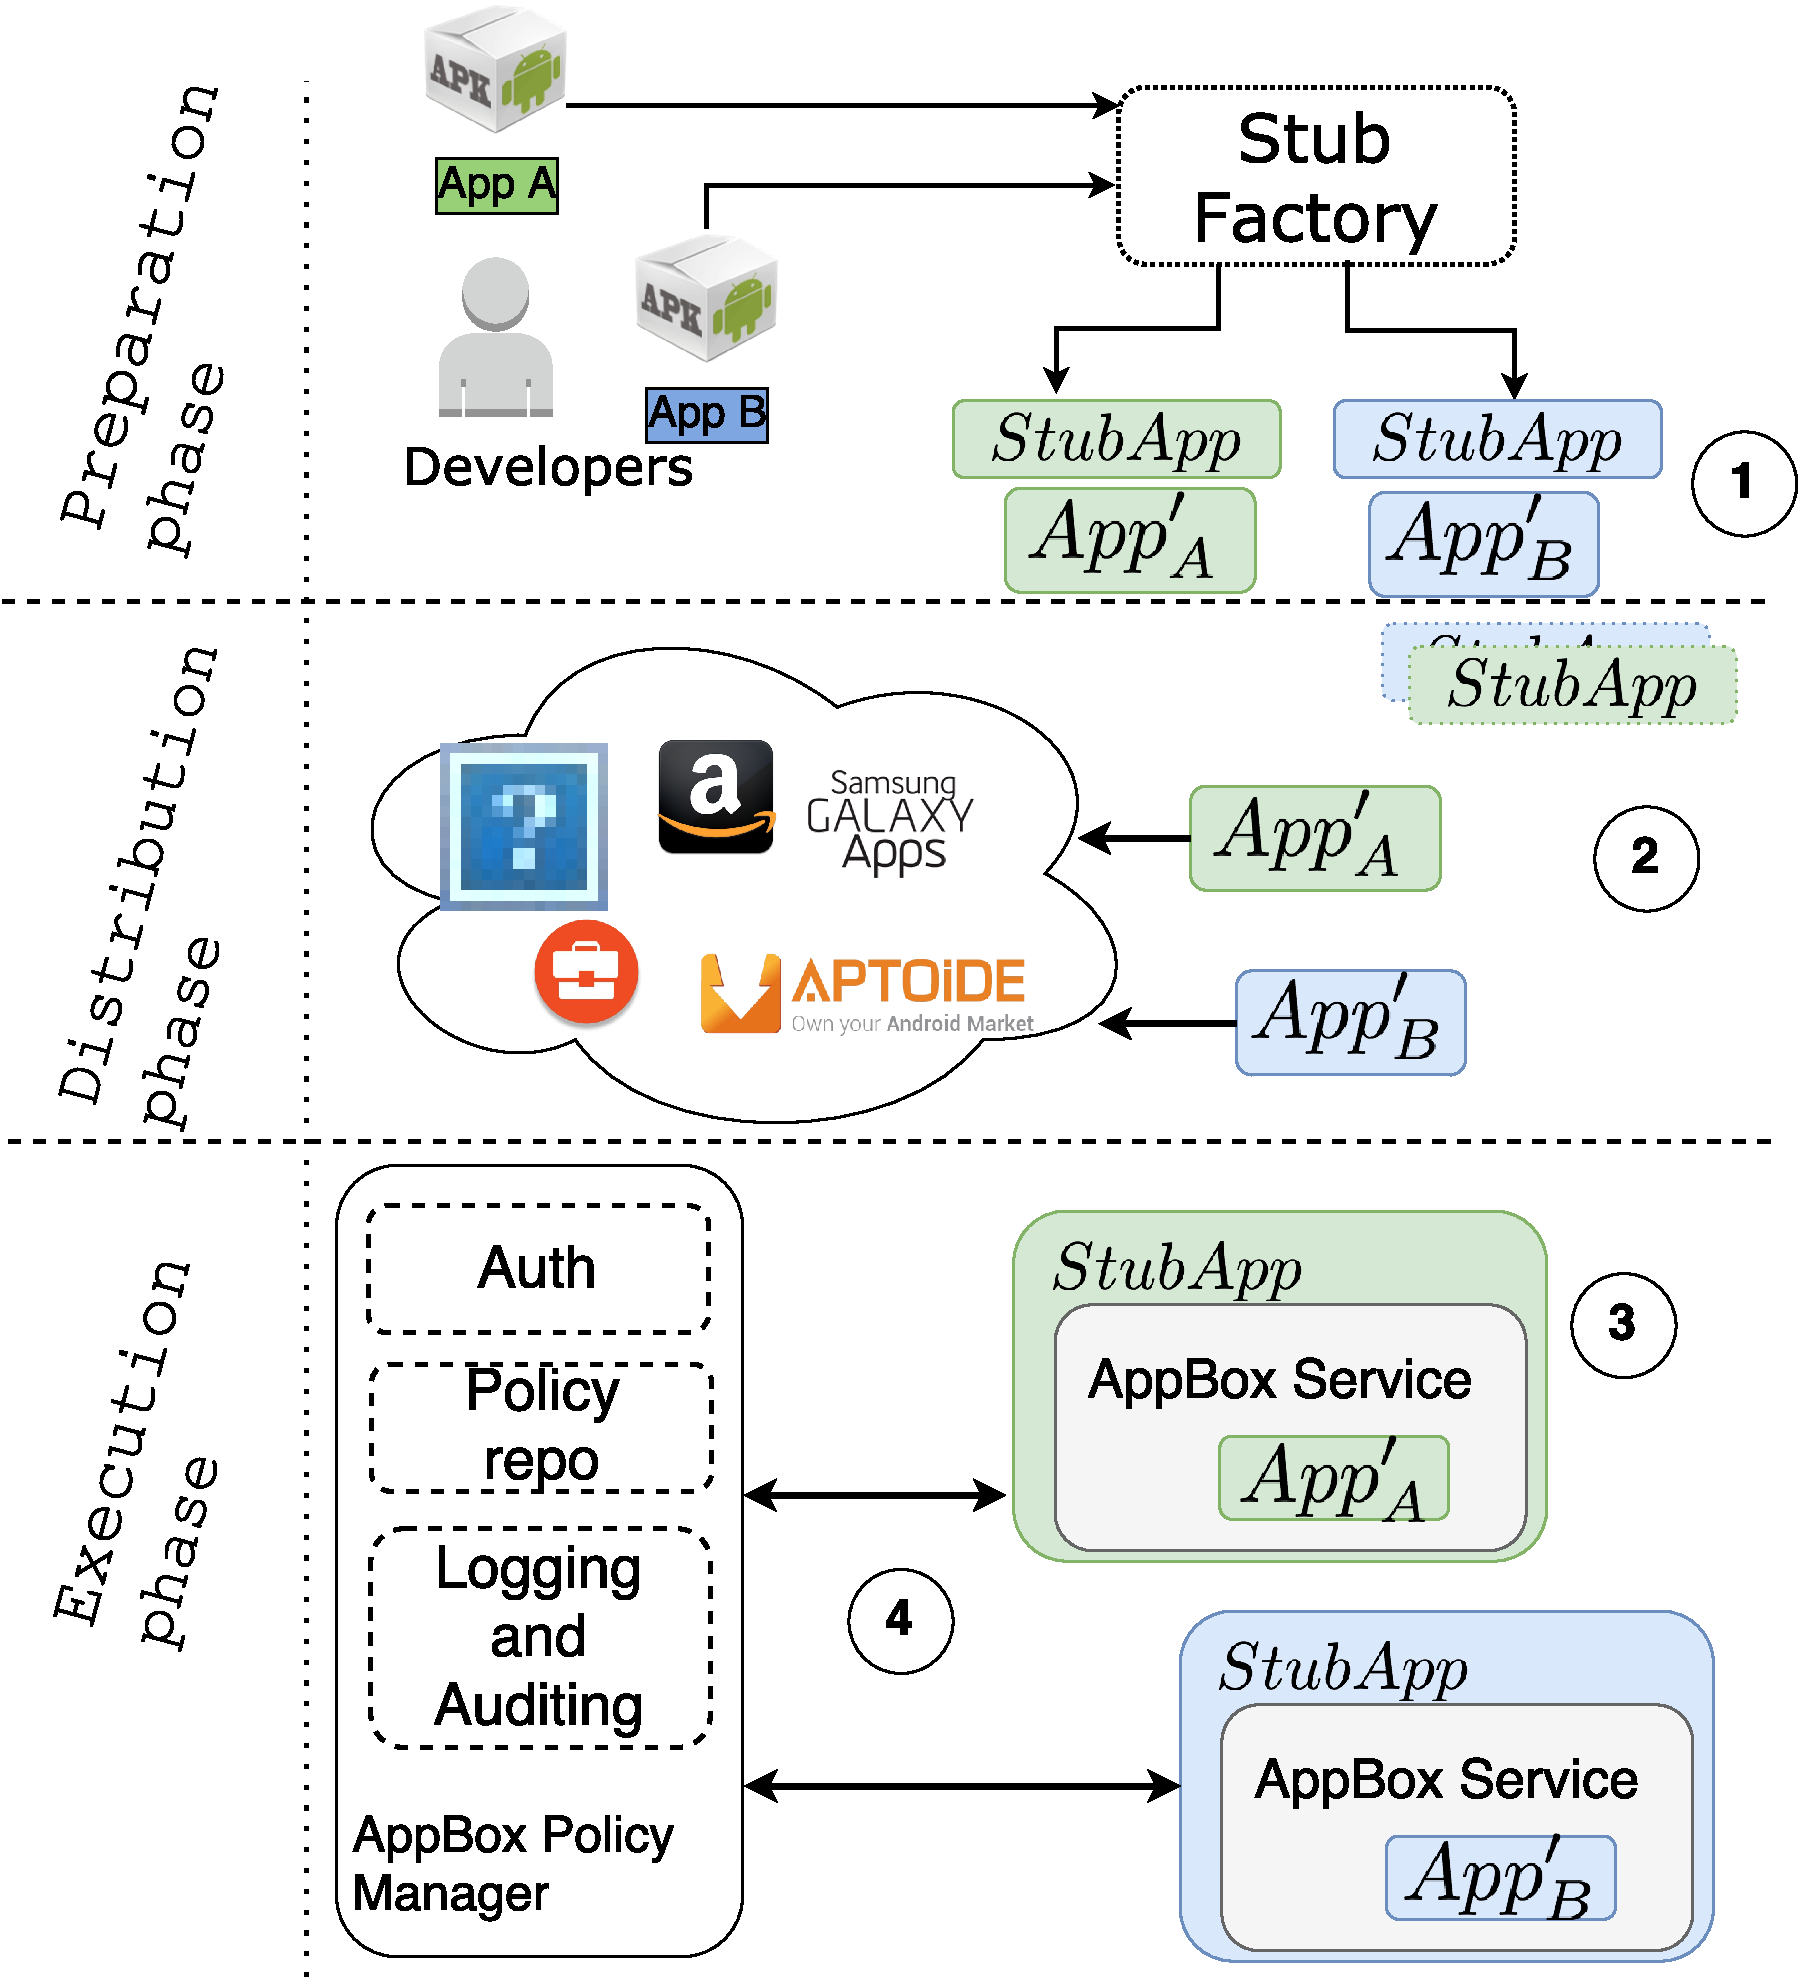
\includegraphics[width=.50\textwidth, keepaspectratio, resolution=600]{phases}
\caption{\asd design phases: Preparation , Distribution and Execution.}
\label{fig:sysdesign}
\end{figure}


\asd workflow consist of three main phases shown in Figure \ref{fig:sysdesign}: \textit{preparation}, \textit{distribution} and \textit{execution}.
During the preparation, the app developer creates the managed app ($App'$) and the \stub (step 1). Then, the developer distributes the managed app via any supported android market (step 2). During the distribution phase of the managed app the 
requested operations are exactly those which are actually followed by developers seeking to distribute their applications, no particular additional steps are required. Finally,  the user installs both  apps ($App'$ and the \stub) on the target device. During the execution phase, the \stub creates a sandbox to execute the managed app. The sandbox is responsible for monitoring the managed app's behaviour and enforce the policies (step 3), specified by the enterprise, offered via \asd Policy Manager instance (step 4). 

In the following, we provide a description of the components involved in each phase.

\subsection{Preparation phase} \label{sec:stubfactory}
To be able to manage an app with \asd, the developer has to create the \stub and a managed app, as shown in Figure \ref{fig:sysdesign}. This steps is performed by the developer using the \stubMaker, a set of python scripts along with a small DEX file containing the actual stub code.   
Another interesting aspect is that because the \stubMaker only operates at the level of the manifest file, the managed app and \stub can be created even if the original app code is obfuscated. 
It is worth noting that none of the existing approaches for app behaviour customisation on stock Android devices, are able to deal with obfuscated apps. 

In the following, we assume that $App$  is an app behaviour that an enterprise wants to customise using \asd. Using the \stubMaker, the developer generates the managed app, indicated as $App'$, and the stub app, indicated as $StubApp$. Finally, both the \stub and the managed app $App'$  must be digitally signed by the developer. 

\begin{figure}[H]
\centering
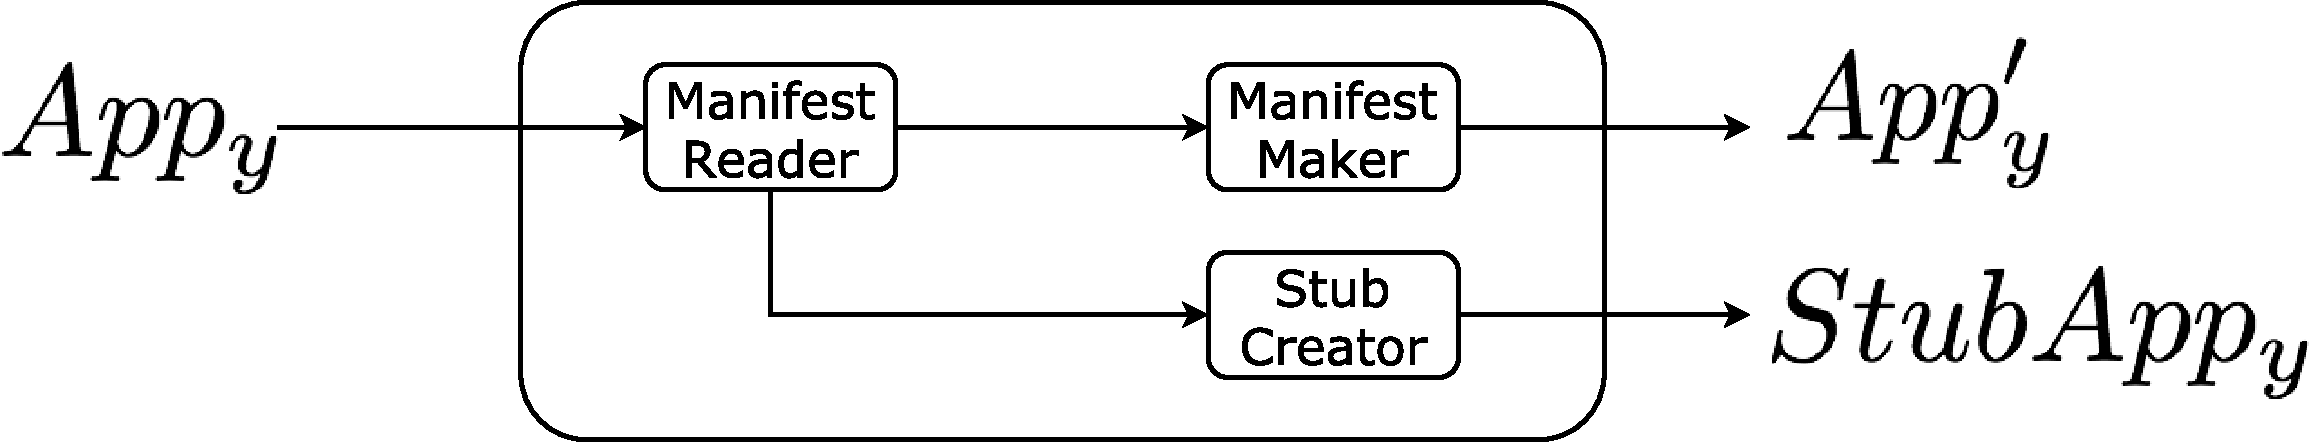
\includegraphics[width=.6\textwidth, keepaspectratio, resolution=600]{stubbo}
\caption{StubFactory and its components}
\label{fig:stubfact}
\end{figure}

As shown in Figure \ref{fig:stubfact}, the \stubMaker first extracts and decodes the Android manifest from $App$ (obtained as APK file) using the \textbf{Manifest Reader}. This component parses the input app's manifest collecting information such as  package name, main activity as well as requested permissions. Furthermore, it checks if the manifest contains components of $App$ defined to run across multiple processes. If this is the case, then the names of these components are added to the manifest of the \stub such that any additional process created by the app will be monitored by a dedicated sandbox instance. It is worth noting that the Android manifest is always in cleartext even in the case of heavily obfuscated apps. \\

Next, the \textbf{Manifest Maker} creates a new  manifest for $App'$ to include both the attributes \shared and \proc. If $App$'s manifest contains the broadcast receiver for the boot completed intent, then this will be removed from the $App'$'s manifest. This is to prevent the situation in which $App'$ might be launched before \stub. 

The last step is to create $StubApp$ through the \textbf{Stub Creator}. This last component first creates the manifest for the $StubApp$ with info previously collected by the Manifest Reader. The  $StubApp$'s manifest will have the same permissions as $App$. By default, $StubApp$'s manifest will have the broadcast receiver component for the BOOT\_COMPLETED system message. In this way, all the \stub installed in a device will start as soon as the booting phase is completed. If the $App$'s manifest also contained this broadcast receiver, then the $StubApp$ will act as a proxy and forward the boot completed intent to $App'$. \\

It is worth noting that $App$ and $App'$ have exactly the same  bytecode. In fact, the \stubMaker only operates on the $App$'s manifest to output \stub and  $App'$.  
The developer is able to create as many \stub as she may need to satisfy customers' requests. In fact, to iterate the preparation steps the developer is asked to create a new certificate, which will be offered to each customer.

Application updates are distributed via the application market as an usual APK file, the developer needs to sign them by the same certificated used at the first place. From the developer point of view, it looks exactly the same when it comes to publish managed app updates. In fact, there is no need to manually propagate those updates to each managed app code. The only step asked to the developer is to create a new managed app by means of \stubMaker components, as discussed before, thus updating an application is trivial as creating a managed one derived from the original application. In most cases there is no need to create a \stub again, this operation is requested only if the app's manifest file has been modified by that update.

In the following, we  discuss the details of the distribution phase.

\subsection{Distribution phase}
Once a developer has built an application she is interested in distributing its product to seeking consumers.  
In this phase the developer distributes applications as usual via any supported market.

There is no specific limit on apps distribution imposed by \asd, in any case who owns the \stub is able to control the associated managed app ($App'$).

\asd does not require any additional user interaction to complete an application update via the employed market and the developer does not need to accomplish any particular operation in order to distributed updates of managed apps. Whenever a new update is developed, in order to distribute it the developer uses the \stubMaker to automatically produce an updated managed app version (same operations done by preparation phase). Thanks to our approach the developer does not need to redistribute the \stub component. 

\subsection{Execution phase}
After the preparation step, both $StubApp$ and $App'$ are deployed on a device running stock Android OS.

The execution of the managed app is done by the \textit{\asd Service}. The \asd Service is a process created by the \stub that loads and executes the code of the managed app $App'$. Because the \stub and the \asd Service share the same process space, it is possible to inject hooks at runtime into managed app's virtual memory (which runs inside the \asd Service). These are the hooks that enforce the desired policy. By sharing the same UID through the use of the \shared attribute, the \asd Service is able to access all the private files of the managed app. In \asd, the managed app is dynamically instrumented by means of functions interposition on both Java and native levels, this enables the enforcement of security policies related to Java APIs and native code. The \asd Service modifies the memory of the managed app to inject hooks capable of intercepting calls to Java methods and to syscalls. The  mechanism is transparent to the managed app and new versions of the target app can be easily managed without the need to change either the \stub or the \asd Service. \\

The biggest technical challenge at this point is to guarantee that the managed app execution will be entirely confined within our sandbox. Android  offers a considerable number of features for apps to communicate with each other and share functionality. These features are accessed through callbacks such as broadcast messages, intents, and IPC. Care must be taken to avoid that these mechanisms can be exploited to let the managed app to execute outside its  sandbox.

In particular,  the exported components of an app, include the main activity that is always exported by default, can receive explicit intents sent by any app. When this happens, usually Android starts the exported component into  a new process. If not handled properly, this could be an issue because effectively could result in a managed app starting in a process outside its sandbox. However, before starting a new process, Android searches if there is already a process where (1) the process name matches the requested component's name; (2)  the process UID is the same as the one assigned to the app in which the target component has been defined. Thanks to the combination of both attributes \shared and \proc the \asd Service is sharing the same process name and UID, hence any intents sent to any exported component of a managed app will be captured and executed within the \asd Service.    


\subsubsection{\asd Policy Manager}
\label{sec:polman}
\asd Policy Manager is console application deployed on the enterprise infrastructure intended to be used by IT administrators. Through the \asd Policy Manager an administration can define new policies and deploy them on the enrolled devices. Once the managed application has been started, the \asd instance manages the authentication process with the Policy Manager. 

It is worth noting that new policies can be dynamically distributed as soon as the enterprise IT department loads them into the policy repository. Furthermore, \asd supports logging and auditing features  that can be configured for each managed app, in order to monitor the status of the app while running.

\subsubsection{\stub and \asd Service} \label{sec:stub}
The \stub is the key component for the realization of the \asd Service. The \stub is responsible for creating the sandbox process where the managed app will be executed as shown in Figure \ref{fig:stubapp}. When a managed app is launched, first the \stub creates the  \asd Service in a separate process (step 1) and invoke the \textit{prepare} method via the Binder to set up the interceptors (step 2). Then, the \stub retrieves the set of policies and the hooking library (step 3) specific to the managed app from the \textit{\asd Policy Manager}. The \asd Service loads the hooking library to  instrument its virtual memory. Once the instrumentation is completed, managed app's code will be loaded by directly invoking the \textit{bindApplication} method exposed by the \textit{ApplicationThread} class. As a result, managed app is loaded and its main activity is executed within the \asd Service (step 4). 


\begin{figure*}
\centering
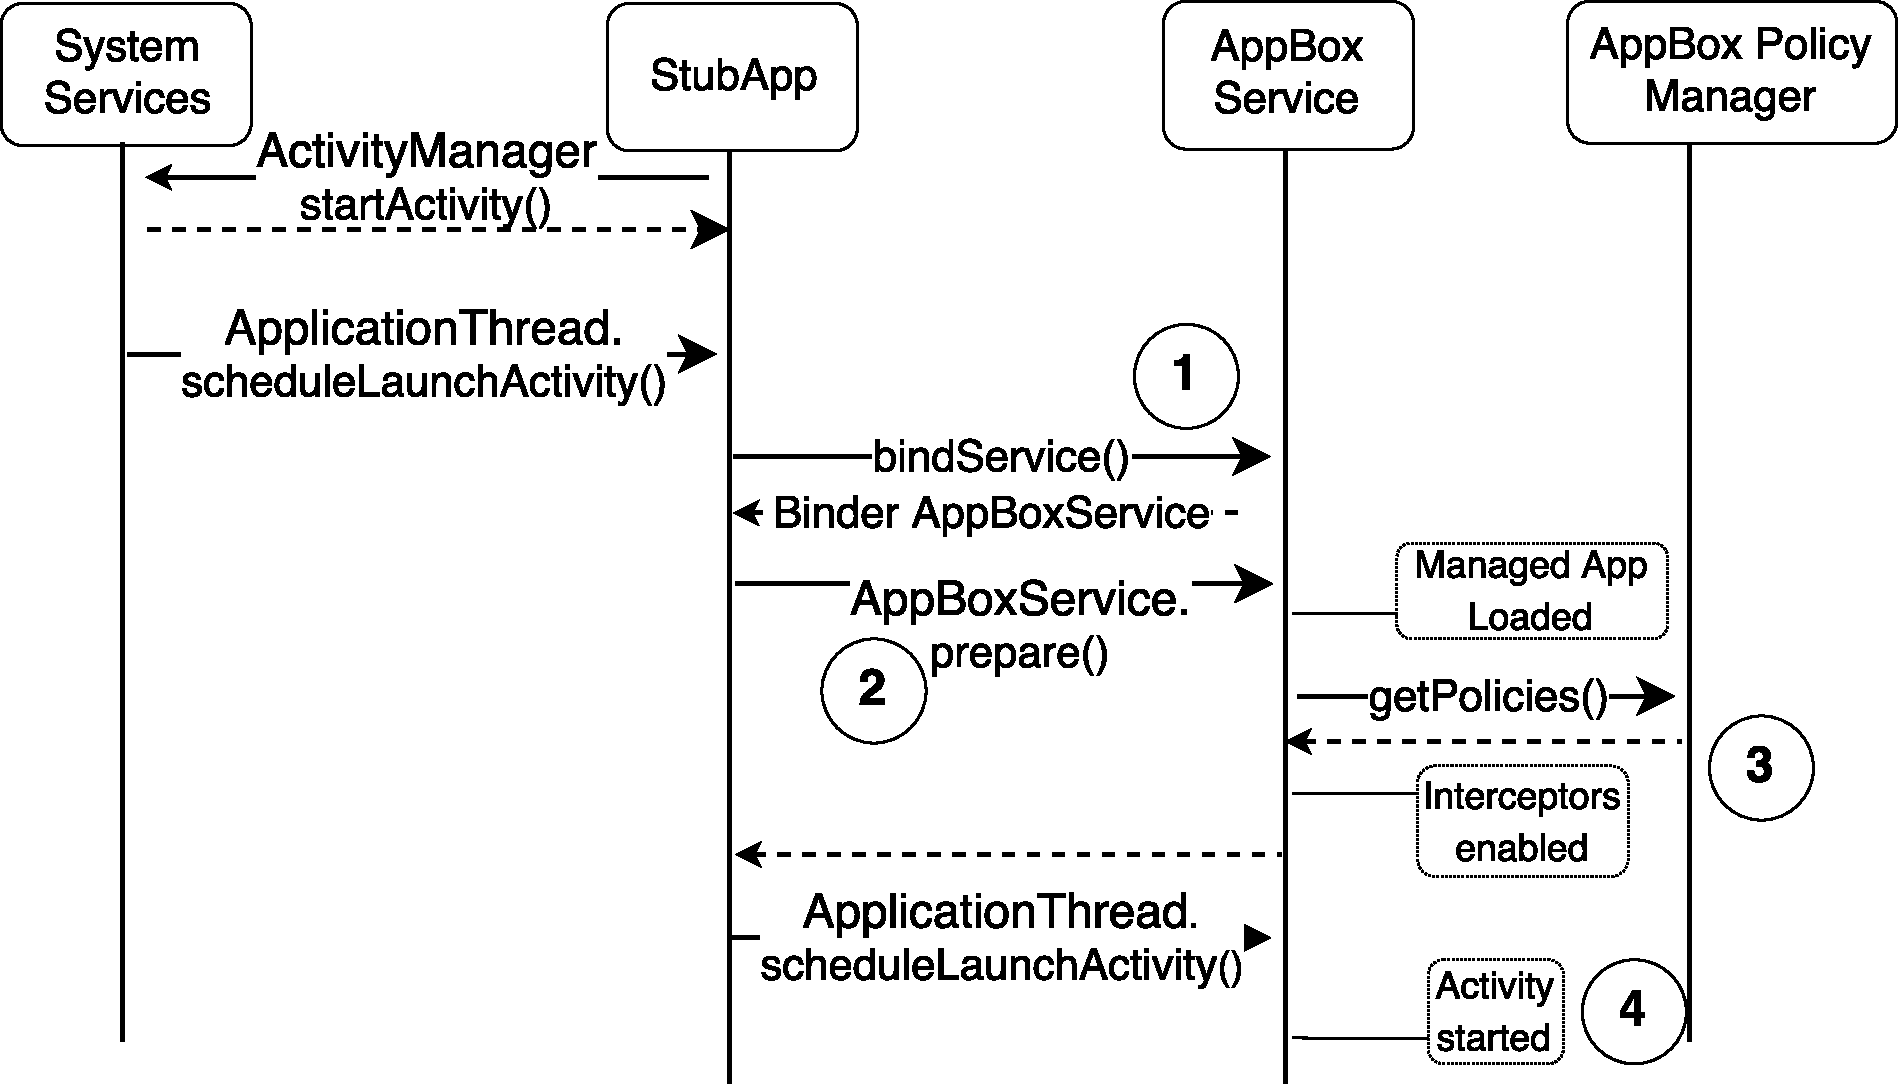
\includegraphics[width=.8\textwidth, keepaspectratio, resolution=800]{lbservice}
\caption{\asd enforcing managed apps}
\label{fig:stubapp}
\end{figure*}

As soon as the library is loaded, its virtual memory is altered to achieve functions interposition by means of different techniques, as detailed in Section \ref{sec:hook}. 

Before the managed app can be executed, the \stub has to create the right Android context for that app. This operation is performed by calling the Android API method \textit{createPackageContext}\footnote{\url{https://developer.android.com/reference/android/content/Context.html\#createPackageContext(java.lang.String, int)}} specifying  the CONTEXT\_INCLUDE\_CODE flag. 
As an entrypoint, the \stub declares in its manifest an \textit{Application}\footnote{\url{https://developer.android.com/reference/android/app/Application.html}} class, that is the first app component loaded by Android before any other app code. 
%In this way, we can make sure that the \asd sandbox is created before the execution of the managed app starts. 
If the managed app has components that need to be executed in different processes then the \stub will start several \asd Services, one for each component of the app. 


\subsubsection{Java and Native Interceptors} \label{sec:hook}
The Java interceptors in \asd are an extended versions of the ArtDroid  hooking framework \cite{costamagna2016artdroid}. However, compared to ArtDroid, \asd Java interceptors are able to hook static Java methods by implementing the approach proposed in \cite{wissfeldcallee}. 
The Java interceptors can operate at the level of Java methods defined within the managed app. We are able to intercept all calls to monitored Java methods including either calls via Java reflection, native code or dynamically loaded code. The intercepted calls are redirected to the specific Policy Enforcement Point (PEP) where the actual user-defined policy is enforced. Java interceptors achieve transparent hooking by means of memory instrumentation. It  fully supports both the DVM and ART Android runtime. The interposition offered by the Java interceptors permits to monitor the access an app performs to  Android APIs to interact with system services (i.e., LocationManager, TelephonyManager) and the Android environment (i.e., Context, SharedPreferences). In Android, apps can also  invoke these APIs from native code via the JNI interface. In addition, in Android native code is allowed to perform direct Binder transactions without invoking any Android Java method. To address this, \asd relies on the Native interceptor to intercept these calls that could bypass the policies defined at the Java level.

\asd offers also  native functions interposition by means of \textit{inline hooking}, a well-known technique~\cite{inlinehook} that basically permits to redirect a function call to another function under the control of a monitor process. In contrast with the GOT patching techniques, \asd can intercept calls to  any native function not only the ones to  global symbols (i.e., calls to functions defined in the same module will not generate entries in GOT). \asd allows to intercept calls to functions like \textit{open, connect, read}, access to the Binder via the \textit{ioctl}, etc. In this way we can  monitor if the managed app tries to access system services directly via native call to the \textit{ioctl} function. Enabling native interceptors is optional. For instance, if an app does not use its own native libraries then native interceptors can be disabled. However, if the managed app dynamically loads a native library then \asd can automatically enable the native interceptors layer.
         

%///////////////////
\iffalse
\begin{figure*}[htbp]
\centering
 % Store largest image in a box
  \savebox{\imagebox{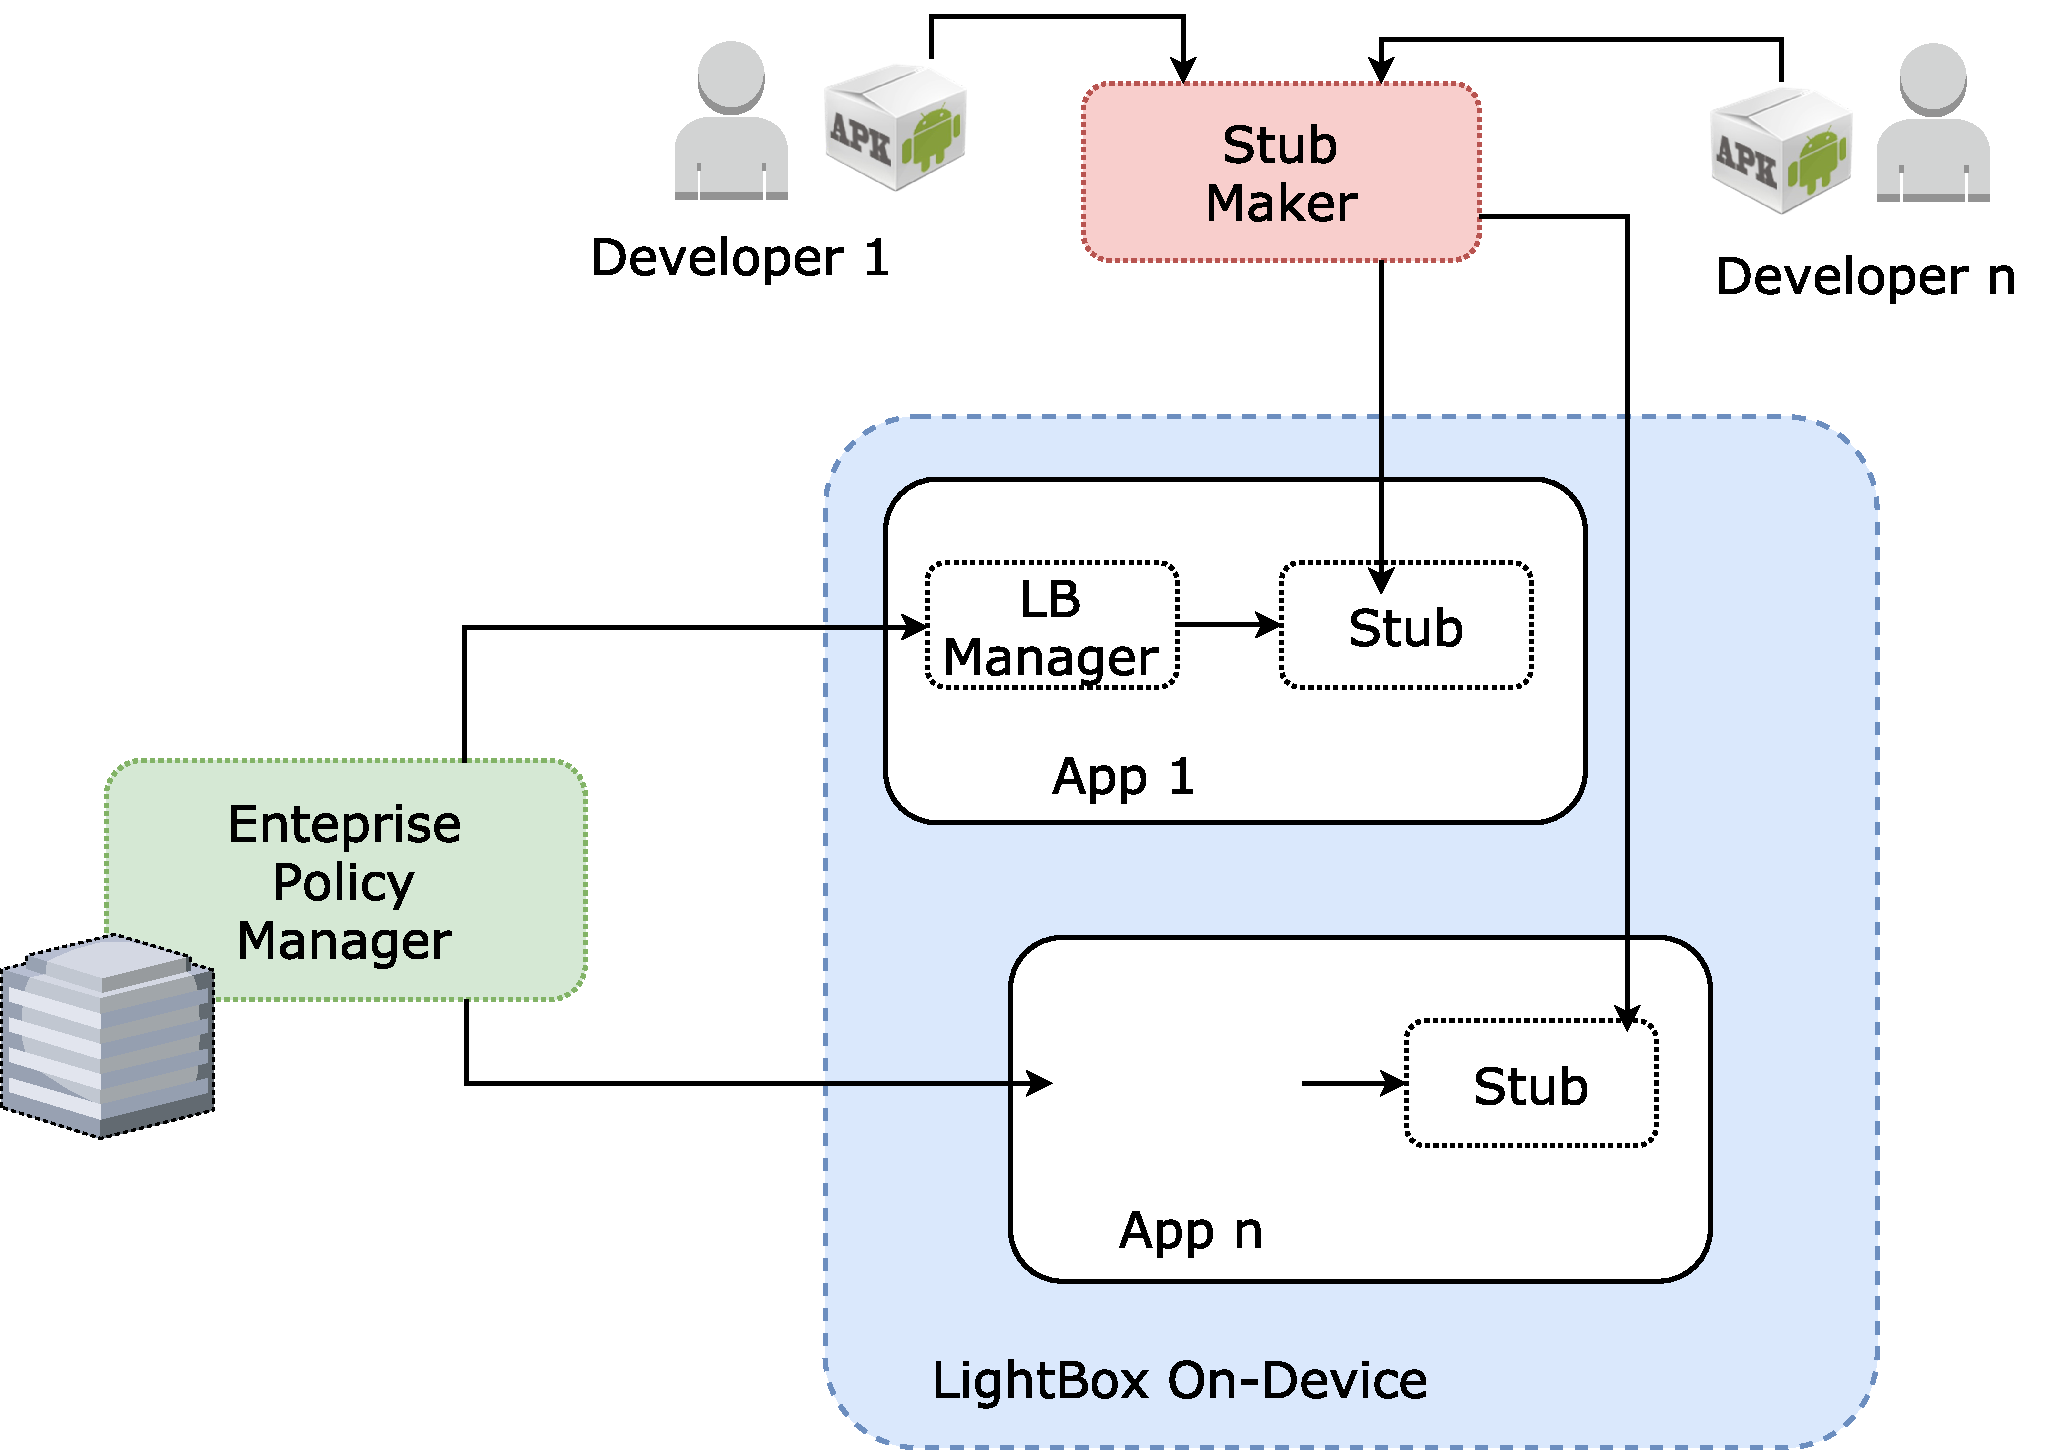
\includegraphics[width=.4\linewidth,height=150pt]{design_overview}}%
  \begin{subfigure}[]{}
    \centering\usebox{\imagebox}% Place largest image
    %\caption{LightBox high level design}
  \end{subfigure}\qquad
  %Nothing
  \begin{subfigure}[]{}
    \centering\raisebox{\dimexpr.5\ht\imagebox-.5\height}{% Raise smaller image into place
      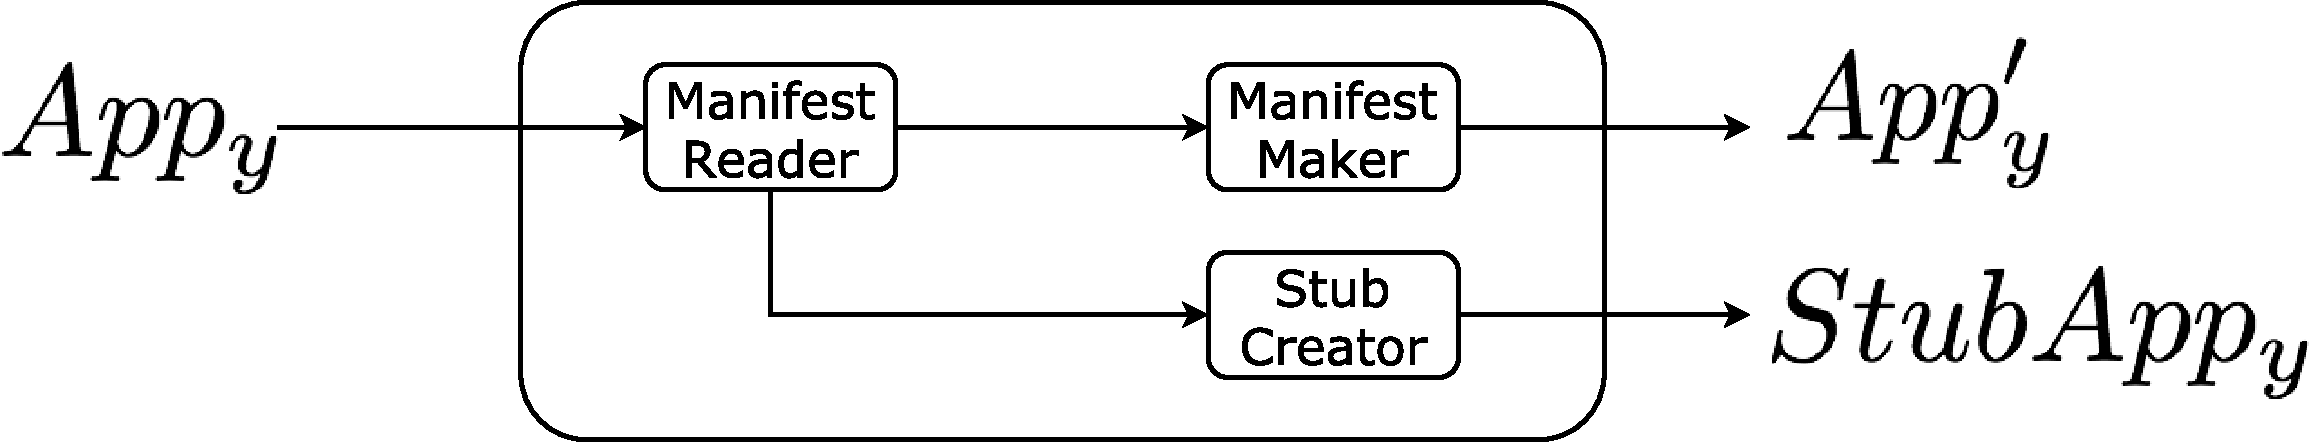
\includegraphics[width=.5\linewidth,height=5pc]{stubbo}}%
    %\caption{StubFactory}
  \end{subfigure}
\caption{\asd (a) system design creation, (b) \stubMaker }
\label{fig:lightbox}
\end{figure*}
\fi
%//////////////////////////////
\iffalse
\begin{figure*}
	\centering
	%\subcapraggedrighttrue
		\begin{tabular}{@{}c@{}}
			\subfigure[a]{
				\centering
            	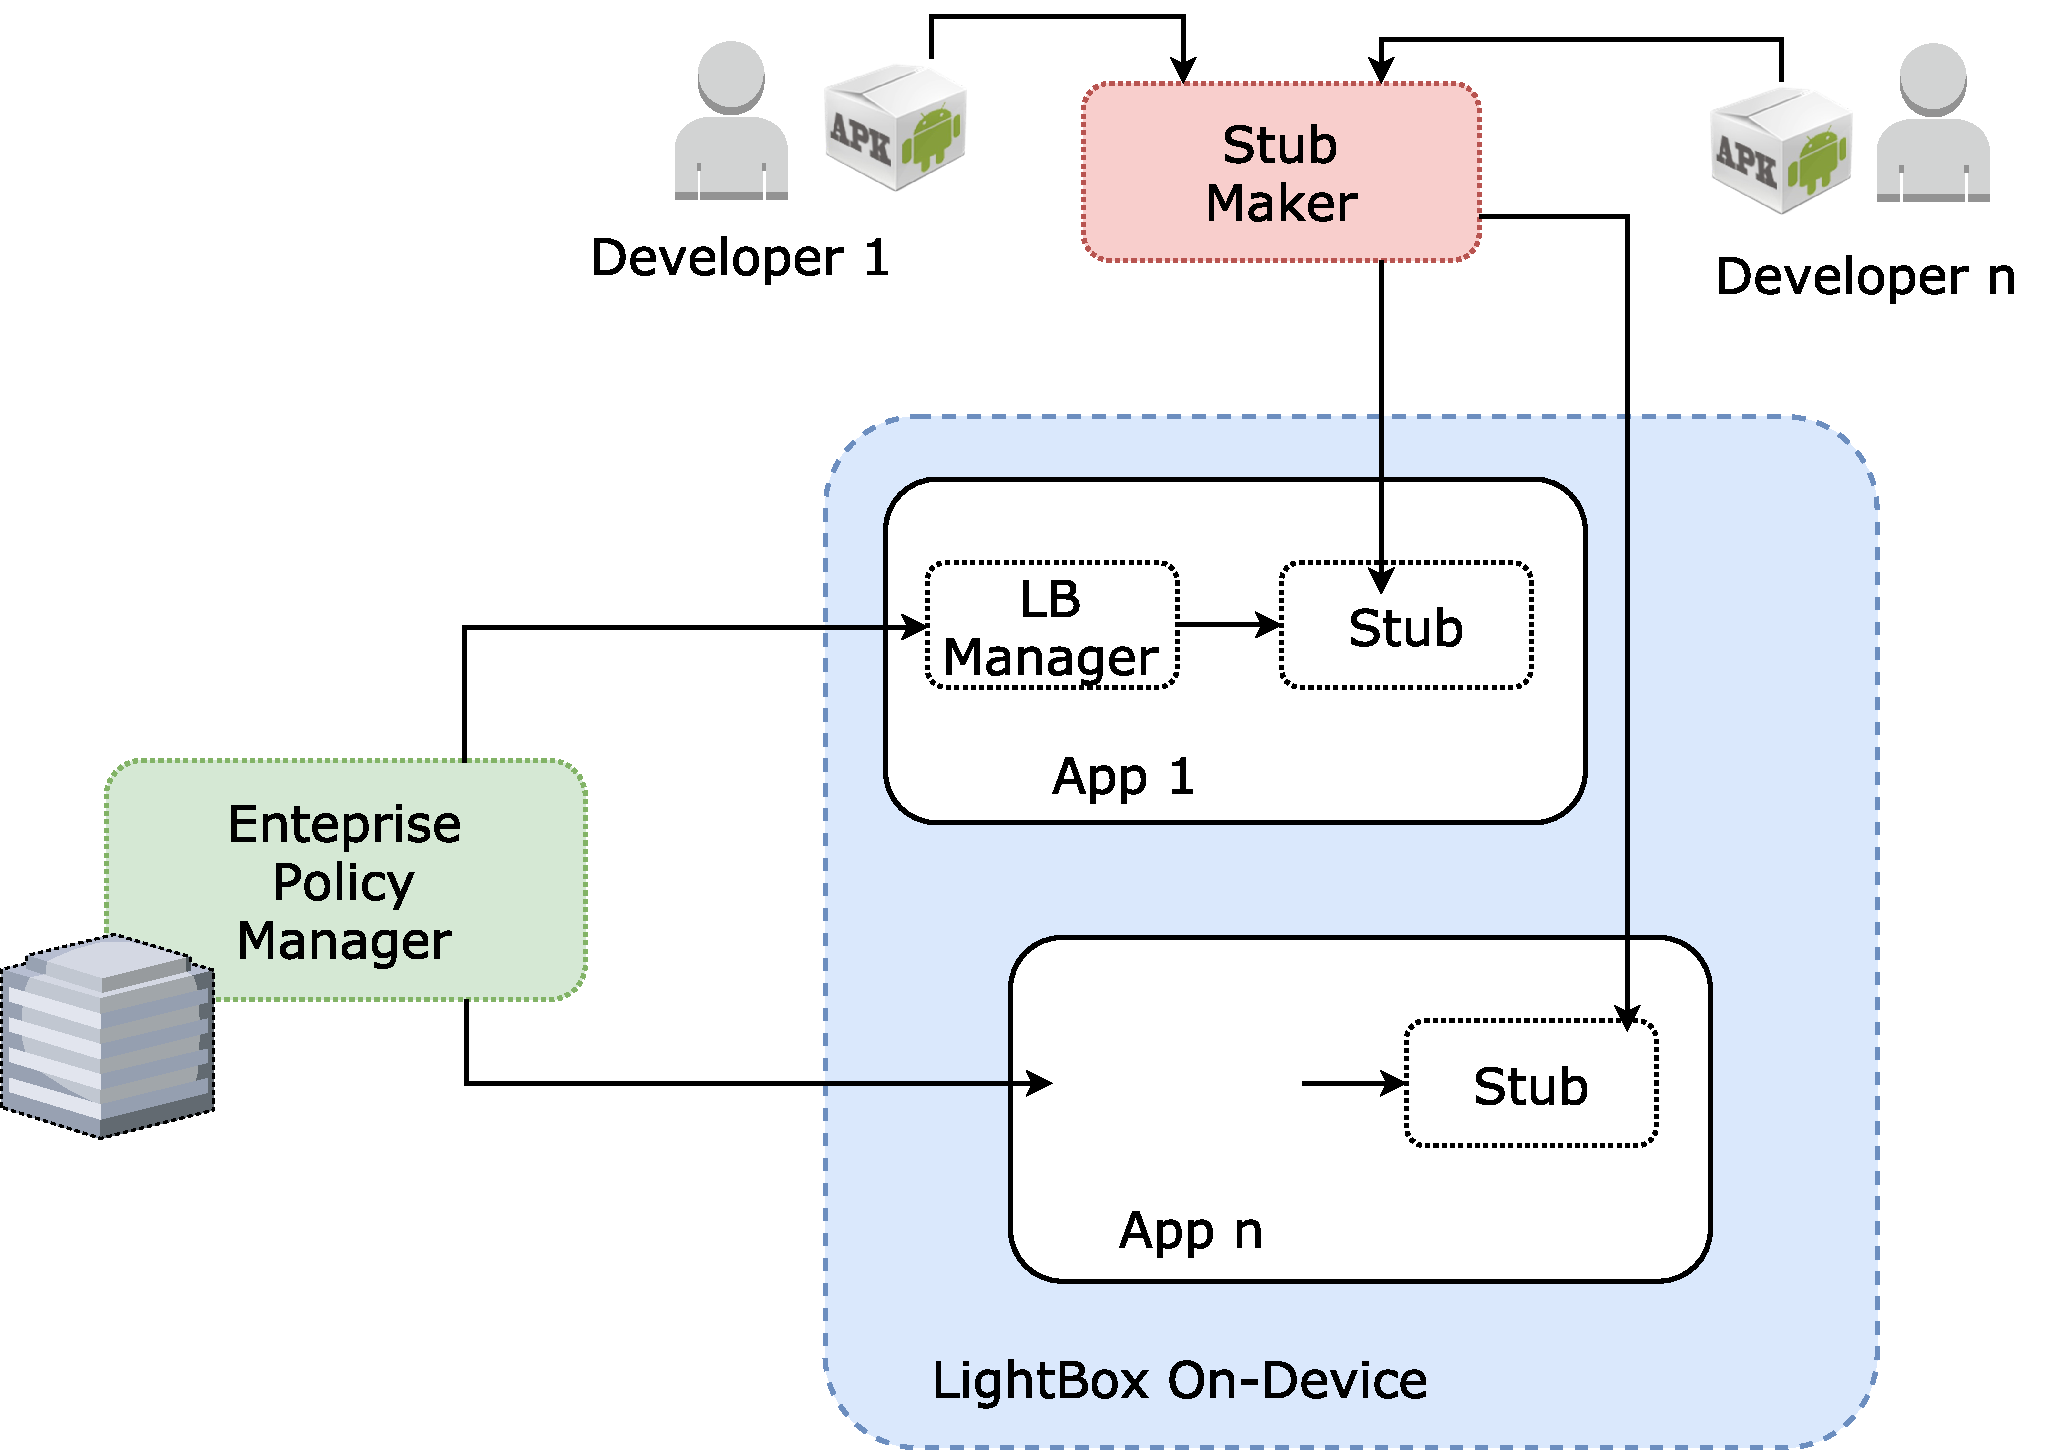
\includegraphics[width=5cm]{design_overview}}
				
		\end{tabular}
		\begin{tabular}{@{}c@{}}
			\subfigure[b]{
            	\centering
                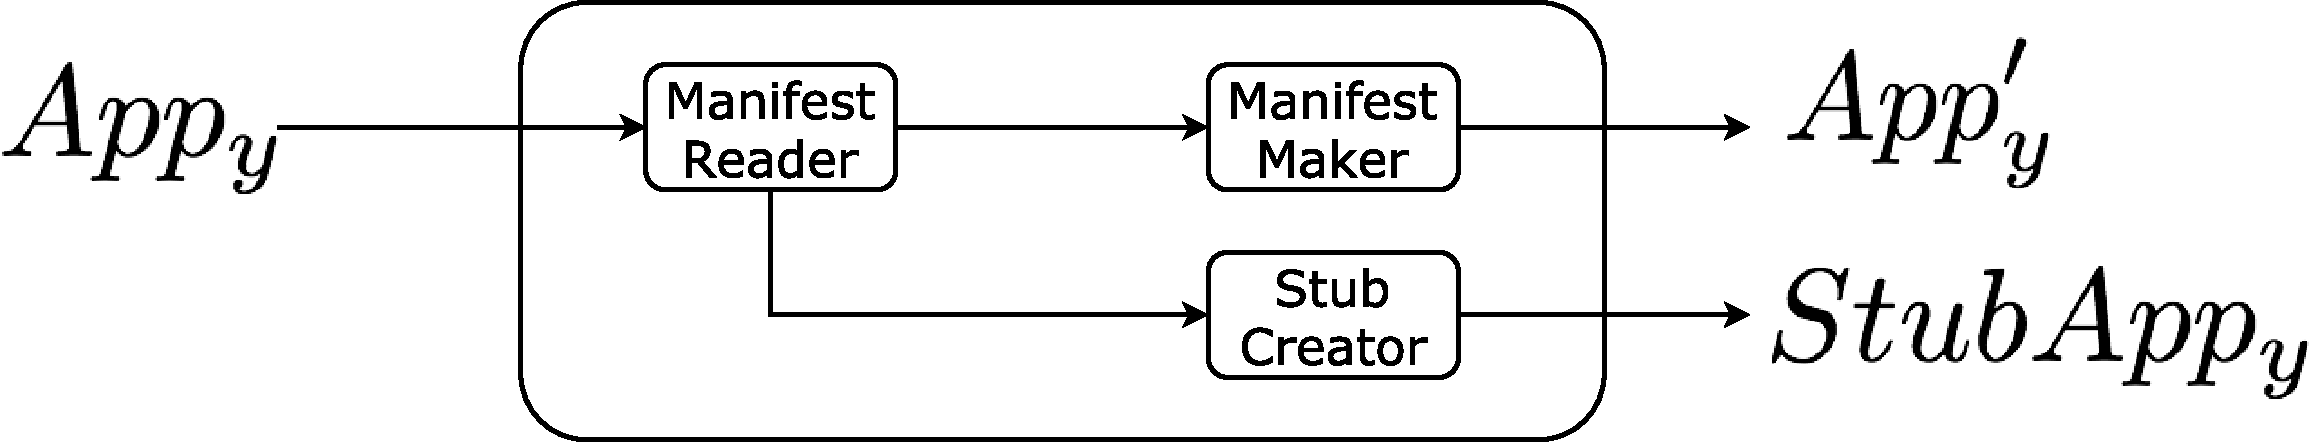
\includegraphics[width=5cm]{stubbo}
				}
			
		\end{tabular}
\end{figure*}
\fi
%--------------------------
\iffalse
\begin{figure*}[!t]
    \centering
    \begin{subfigure}[b]{0.47\textwidth}
        \centering
        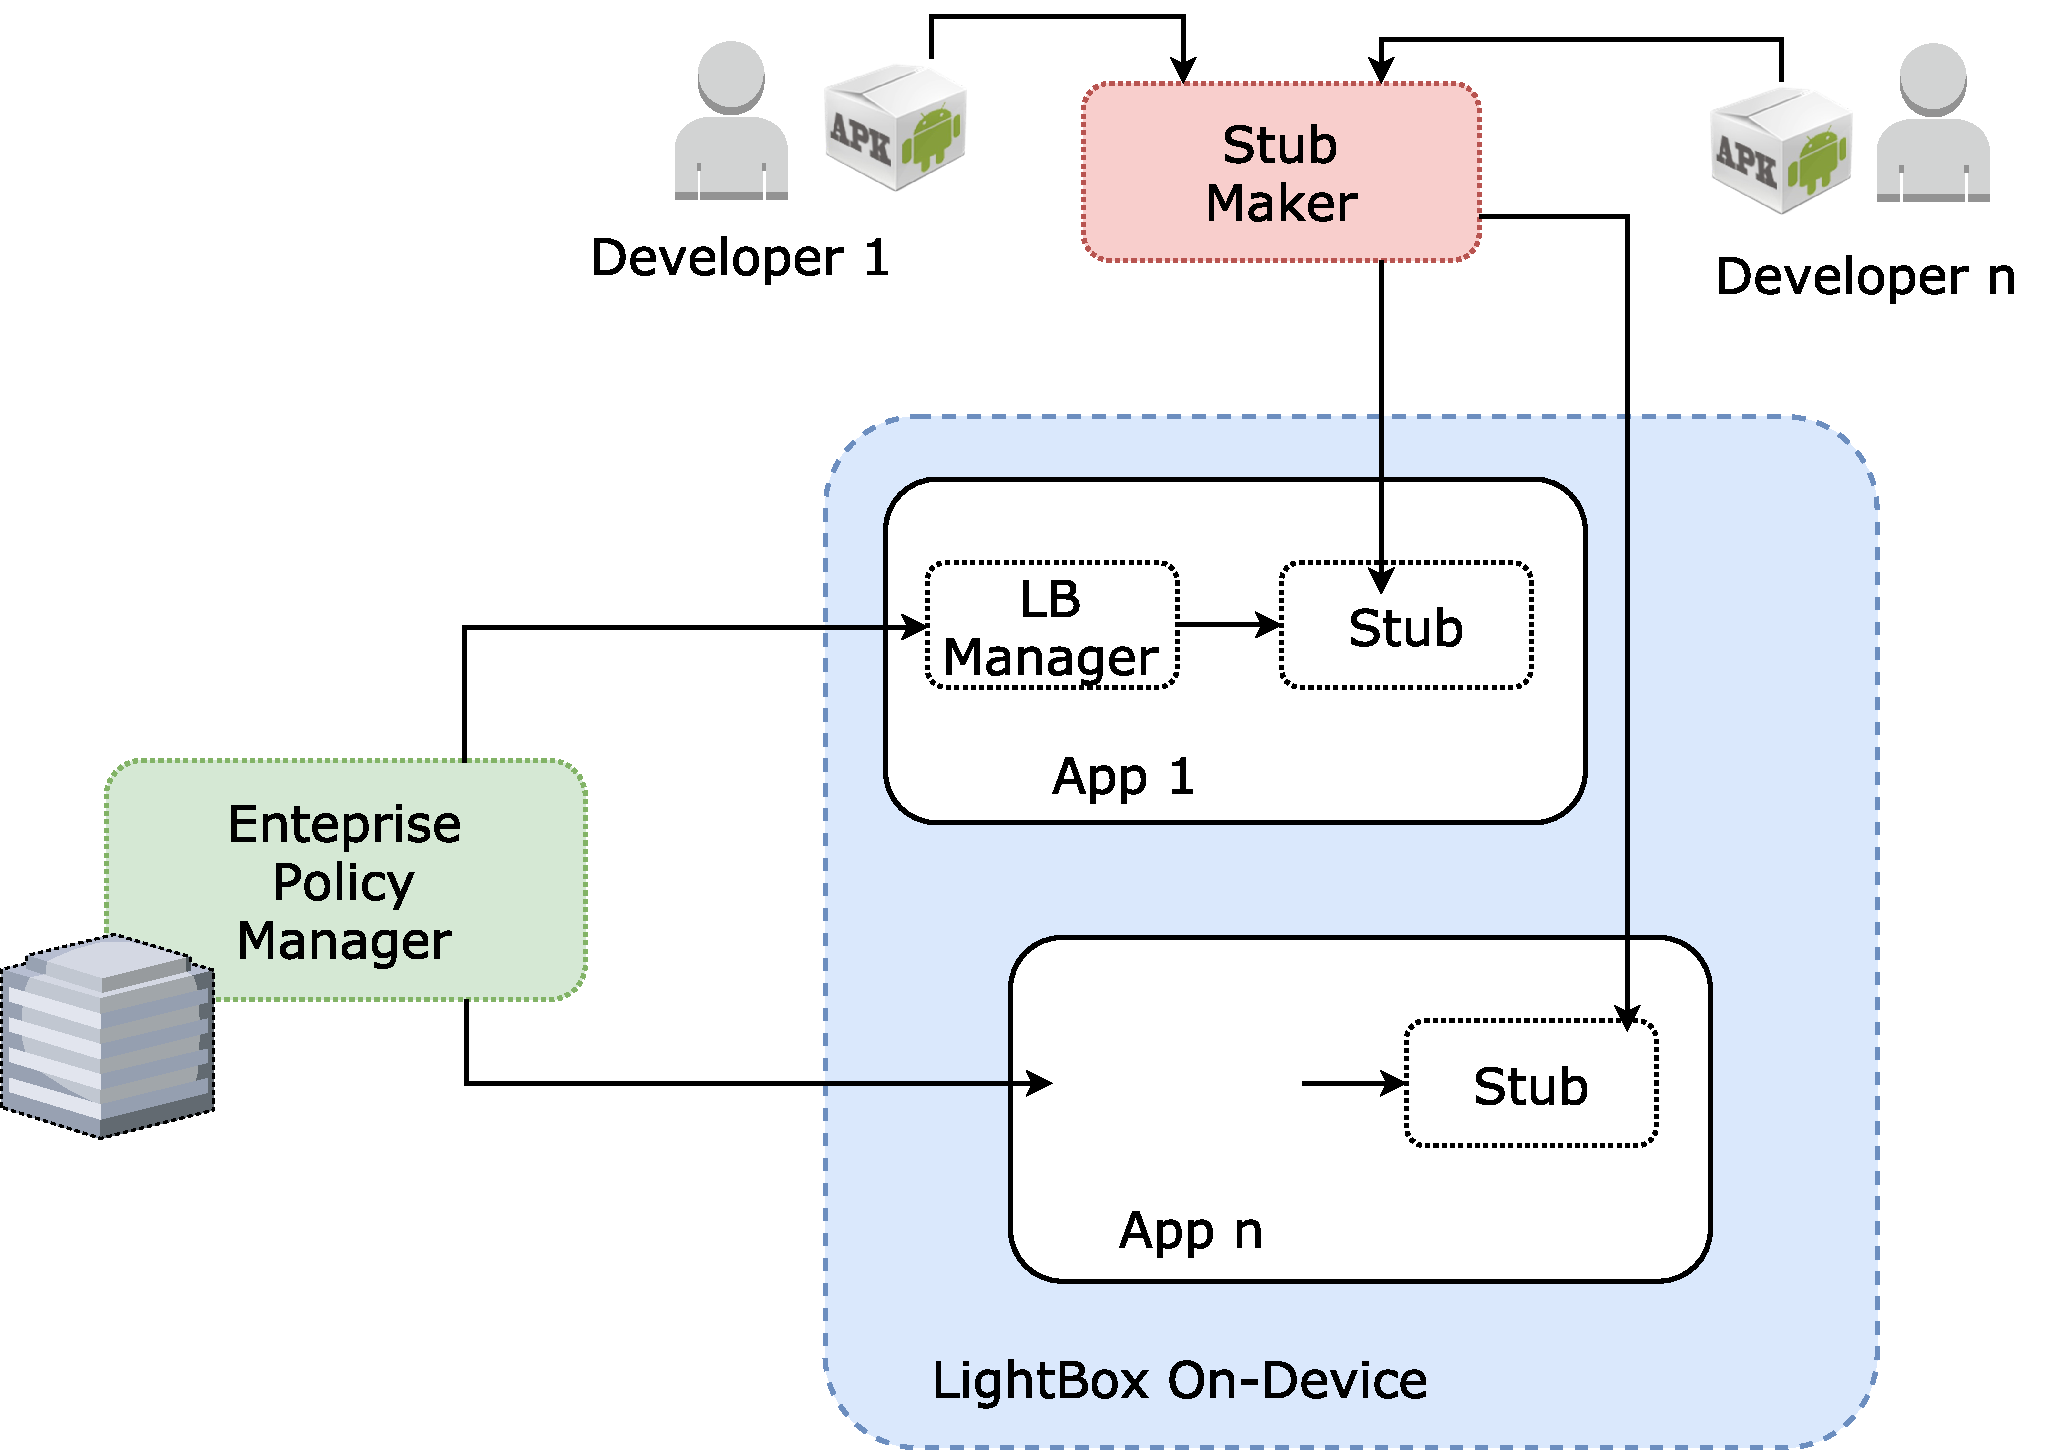
\includegraphics[width=\columnwidth]{design_overview}
        \caption{}
        \label{fig:design_overview}
    \end{subfigure}%
    ~
    \begin{subfigure}[b]{0.29\textwidth}
        \centering
        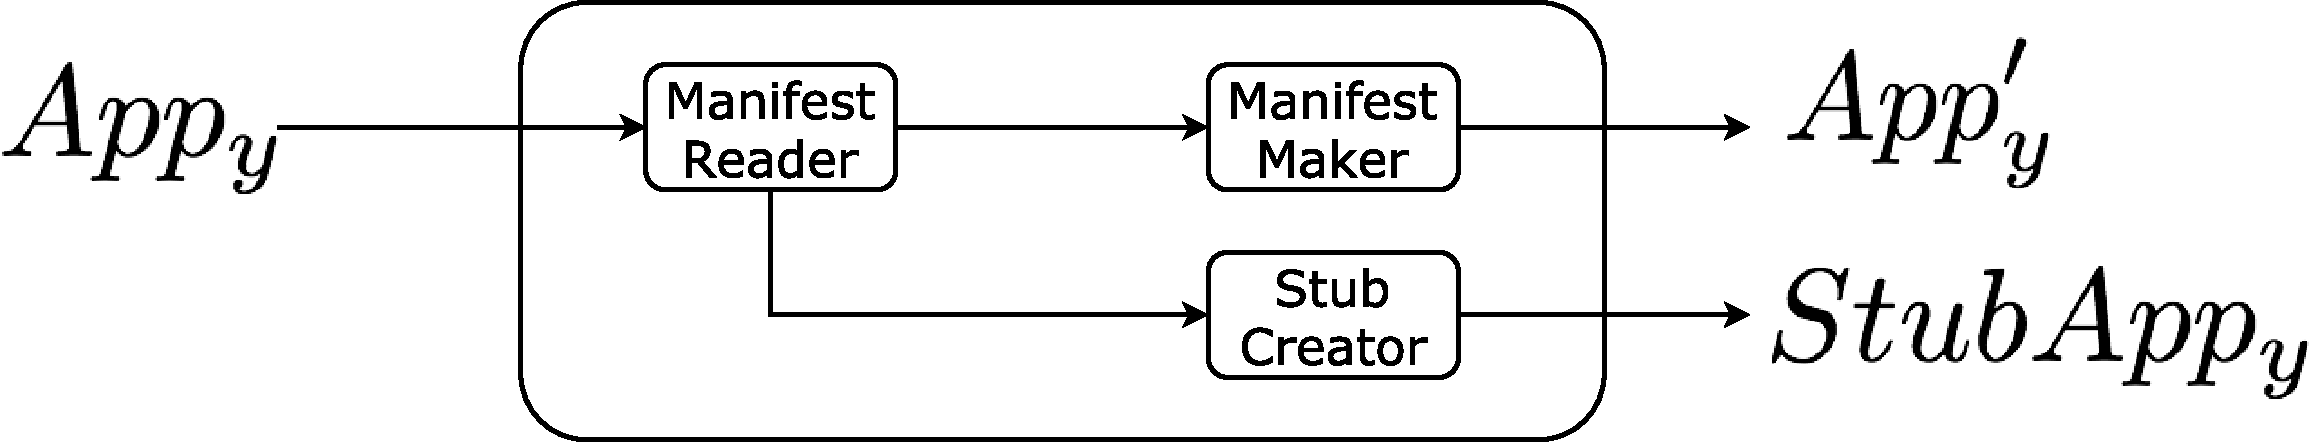
\includegraphics[width=\columnwidth, height=.1\textheight]{stubbo}
        \caption{}
        \label{fig:stubbo}
    \end{subfigure}%
    \caption{a) ... b)....}
\label{fig:example}%
\end{figure*}
\fi
%------------------------------

\section{\asd Policy}
\label{sec:policy}
In this section, we first present the \asd policy language for controlling app's behavior during its execution. Afterwards, we will present  how to define in \asd policies discussed in our application scenario ( see Section \ref{sec:app-scenario}). Finally, we provide some details on how policies can be automatically generated. 

\subsection{Policy Language}
Figure \ref{fig:lang} shows the the syntax of \asd policy. Policies are identified by a name and they define what \textit{operation} a \textit{Requester} application can execute on a \textit{Resource}. In our prototype we defined two sets of \textit{operations}: the first set contains getter methods that return data from the Resource to the Requester; the second set contains  setter methods where data is being passed by the Requester to the Resource. Moreover, \asd offers the possibility to define policies on events (i.e. boot completed, app installed, app running, etc\ldots). The operations defined in the policies are then mapped to Java methods or native functions that \asd will interpose at runtime to enforce the policies.

\begin{figure}[ht!]
\centering
\lstinputlisting[language=Java]{mysnippets/lang.txt}
\caption{\asd Policy Language}
\label{fig:lang}
\end{figure}

In \asd, a Resource identifies any sensitive data which could be retrieved via either Android middleware API (i.e., location, contact, camera) or native code (i.e., sensors, socket, microphone). 
 
The \textit{have to perform} clause  specifies which actions have to be performed if this policy is enforced. These actions are mappped to a set of functions to control the app's behavior (i.e., filtering, anonymisation, etc.) and to change the values of the parameters of the operation being executed. An action is a callback that is registered by \asd to dynamically forward the execution to the corresponed function and  can operate on both input parameters and returned values. 

A policy can have an optional clause \textit{if} that defines a condition that must be verified before the specified action is performed. Otherwise, if the condition is not true, the action specified in the policy is not executed. 


\subsection{Fine-Grained Access Control Policies}
\label{sec:finepolicy}
We begin with some examples of policies for fine-grained control over apps accessing user data or using network access. Any  access to a protected resource is intercepted by the hooking mechanism and diverted through a custom user-defined control code. \\
As discussed in Section \ref{sec:app-scenario}, the enterprise $Ent$ wants to enforce fine-grained app-level policies. In this scenario, $Ent$ wants to protect business data (i.e., contact and calendar) against unauthorized operations according to custom corporate-level policies and protect the managed app enforcing integrity checks at runtime. Moreover, $Ent$ wants that any connection made by a specific set of apps makes use of a secure channel (i.e., TLS) thus reporting any connection which makes use of insecure transport system like HTTP. The enterprise's requirements can be expressed by policies shown in Figure \ref{fig:policies}. \\

\begin{figure}[ht!]
\centering
\lstinputlisting[language=Java]{mysnippets/policies.txt}
\caption{\asd Policies}
\label{fig:policies}
\end{figure}

\textit{MicPolicy} in Figure \ref{fig:policies}, is quite straightforward: any request for accessing to microphone capabilities made by managed apps is restricted by the policy such that \asd intercepts the request and checks for the specified condition (if clause) , if it is validated then the access is denied. Another similar policy is \textit{LocPolicy}. Such policy permits to avoid location information leak potentially made via apps during working hours. The artificial value returned by \asd is totally controllable by the user, by default \asd returns an existing location chosen at random among a user predefined set of positions.

The policy \textit{ContPolicy}, line 9,  permits to achieve a content provider isolation for an \asd managed app. In this specific case, $Ent$ wants to isolate corporate business contacts sharing them only across authorized apps that have been register throught the \asd Enteprise Policy Manager (see Section \ref{sec:polman}). Moreover, the $Ent$ wants to specify particular criteria that must be respected to allow to the managed app to access business contacts data. In particular, the policy ContPolicy operates as following. The requested operation getContact indicates that any kind of attempt to retrieve the user contacts list must be intercepted and monitored by \asd. Then, for each intercepted operation the specified conditions must be verified. The user-defined isWorkHours() function returns True whether the actual time is within the current working time, False otherwise. If isWorkHours() returns True then the specified action is executed. Otherwise, the execution flow will continue as if \asd was not in place. Thanks to this policy, $Ent$ is allowed to specify a customizable fine-grained access policy enforcing access to the isolated corporate contact provider exclusively to apps managed via \asd.


The policy \textit{HTTPPolicy} (line 13), permits to filter out any connection that is being made via HTTP protocol. Connections instantiate by the managed app can be intercepted and monitored by either hooking the appropriate Java level APIs or intercepting native layer functions if needed. The policy specifies that any operation recognized as an attempt to create a connection has to be intercepted and monitored by \asd. The condition verifies whether the request is made during the working time. In this specific case, $Ent$ wants to deny insecure connections made via HTTP protocol. \\

As an example of a policy defining an artifact Resource, \textit{CopPolicy} is presented. It enables the enterprise to specify a custom integrity check to be enforced before the managed app start its execution. Given a specific app, the enterprise wants to verify that its bytecode has not been tampered with. Here we stress that \asd does not require to modify the app's bytecode, thus its checksum value does not change. Thanks to this policy, before each execution of the managed app \asd
computes the app's bytecode checksum value to guarantee that it has not been tampered with. \\
In the following we present and discuss how \asd policies can be automatically generated by the enterprise.

\subsection{Policy Generation}
In this section we present how \asd policies can be automatically generated by extracting information from the policy specification file. The overall procedure of policy creation is presented by Figure \ref{fig:genpolicy}. The policy generator takes as input the policies specification, the sets of Resource that $Ent$ wants to protect (Res.) and the information about what operation is offered by what Resource (Op.). In our current prototype, we selected sensitive resources (i.e., contacts, location, internet access) and we grouped them by the relative requested permissions. Then we used the information offered by PSCout\cite{au2012pscout} to aggregate Android APIs in terms of which permissions are needed by them. At this point, in our prototype we manually selected which API methods belong to a Getter or Setter operation. By doing this we created a mapping between Resource, Operation and the API methods which are offering capabilities to execute that specified Operation on that specified Resource. It is worth noting that $Ent$ can simply extend those sets including any resource that wants to enforce, as presented for \textit{CopPolicy}.
In Table \ref{tab:map} we reported the mapping was used for the policy HTTPPolicy. For the sake of understanding we included only the Android APIs offering HTTP capabilities as they are suggested by the official Android developer guide\footnote{\url{https://developer.android.com/training/basics/network-ops/index.htm}}. The policy expressed by the specification shown in Figure \ref{fig:policies} line 13, produces according to the requested operation on the specified Resource the interposition of the API methods listed in the third column of Table \ref{tab:map}. \\
Finally, the policy generator produces as output the executable file encoding the corporate app-level policies that will be loaded by \asd to enforce at runtime the policies taken as input by the generator.

\newcolumntype{L}[1]{>{\raggedright\let\newline\\\arraybackslash\hspace{0pt}}m{#1}}
\newcolumntype{C}[1]{>{\centering\let\newline\\\arraybackslash\hspace{0pt}}m{#1}}

\begin{table}[!htbp]
%\begin{minipage}{.5\textwidth}
\caption{HTTP-Policy Generation - Intercepted APIs}
\label{tab:map}
\centering	
\begin{tabular}{@{}cc@{}} \toprule
Operation & API to hook (clsname, mname) \\
\cmidrule(l){1-2}
\multirow{2}{*}{createConnection} & (HttpURLConnection , $<init>$)  \\
 & (URL , $<init>$)  \\
 & (URL , openConnection) \\
\bottomrule
\end{tabular}
\end{table}


\begin{figure}[H]
\centering
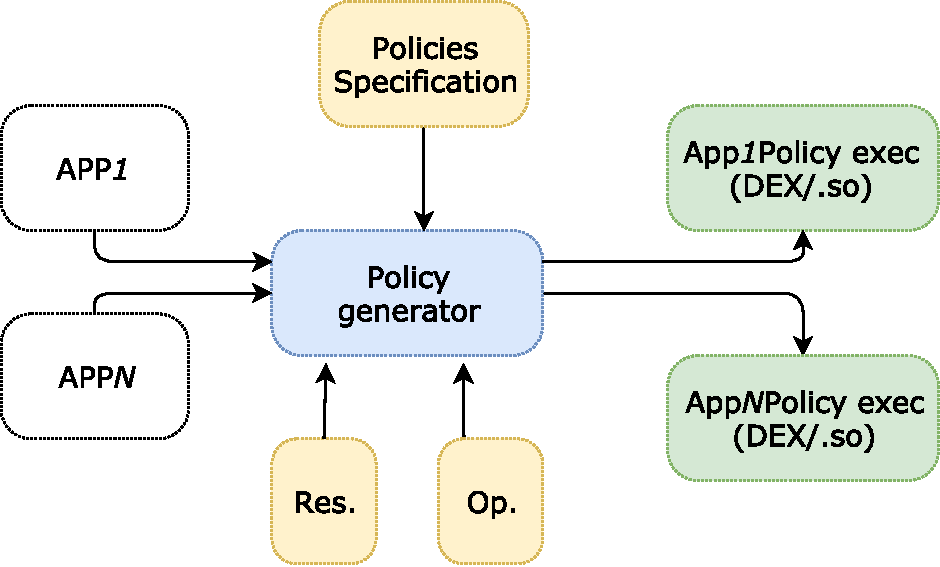
\includegraphics[width=.55\textwidth, keepaspectratio, resolution=600]{policy_gen}
\caption{Policy generation mechanism. Res.: sets of Resource, Op: sets of operation}
\label{fig:genpolicy}
\end{figure}


\section{Evaluation}
In this section, we discuss the evaluation we carried on to test performance overhead, robustness, applicability and effectiveness of \asd. For our tests, we used a Nexus 5x (64bit) device running stock Android Oreo version 8.0.0.

\subsection{Performance Overhead}
To evaluate \asd performance penalty on managed apps, we used benchmark apps and our custom micro-benchmarks. As benchmark apps, we used Quadrant and  Vellamo\footnote{\url{https://play.google.com/store/apps/details?id=com.quicinc.vellamo}}: the former was selected because it has been used in other related works \cite{russello2013firedroid,backes2015boxify,bianchi2015njas} so it will make easier to compare the performance of \asd with similar approaches; the latter is a highly accurate benchmark developed by Qualcomm and contains a benchmark specifically intended for stressing the Binder communication channel. Given that the Binder is the most common means of communication for Android apps, it is important to measure the overhead \asd  introduces. Moreover, we executed the \textit{webview} package of Vellamo that contains various benchmarks for Android's Webview API. We included this test in our experiments because a huge number of apps are either entirely developed within a Webview or specifically use its features. 

As shown in Table \ref{tab:perf1}, the impact of \asd on the total score produced by the benchmarks is low. The test marked as \textit{total} reports the cumulative score that the Quadrant benchmarking app produced when executed, while the I/O test were oriented to stress operations of reading/writing from/to disk. The worst score, of about 15\% is low when compared to similar works, and can be  attributed to the I/O test. It is worth to note that in both scores, \asd overhead is much lower than the one introduced by solutions like Boxify and NJAS in equivalent tests. In fact employing a light-weight in-memory hooking mechanism, instead of ptrace, and 
avoiding critical services emulation via Broker component, \asd reduces remarkably the performance costs requested for monitoring the target app.

As for the performance penalty introduced in the Binder communication (indicated as multi-core in Table \ref{tab:perf1}), the score indicated by the Vellamo benchmark is really low (up to 1\%) due to the fact that \asd does not need to perform extra marshalling operations. It would have been interesting to report the same tests for  NJAS and Boxify\footnote{At the time of writing this paper, a version of Boxify was released but it's not based on the isolated process mechanism as described in \cite{backes2015boxify}} 
but both systems were not available to us at the time of writing. 

To understand the performance implication of \asd on method invocations and function calls, we developed a synthetic app in order to perform a micro-benchmark testing performance penalties when executing Java and native method calls. The micro-benchmark tests the most significant native functions by means of \asd native interceptors. In Table \ref{tab:perf_native}, we report  the overhead introduced by \asd when hooking  functions in libc (shown in the first column). In the same table, we also compare our overhead with  Boxify performance overheads as reported in \cite{backes2015boxify}. As the results show, \asd's performance overhead is significantly less than Boxify's, mainly because of the extra rounds trip needed by Boxify to forward to the the Broker component each intercepted calls which costs in average $\approx$ 100 $\mu$s of delay for each call. 

Table \ref{tab:perf_api} reports the results for the overhead introduced by \asd when interposing Java Android APIs, Table \ref{tab:perf2} presents hooks that were in place during our experiments. Results shows that the performance penalty introduced by \asd's API Hooking, while not being ideal, is acceptable. It is worth noting that micro-benchmarks test listed in Table \ref{tab:perf_api} in some cases (i.e., openFileOutput and Create File) are responsible for triggering multiple hooks. A very fast operation such creating a new File object has a performance degradation which cost in average 10 $\mu$s of delay. The \asd Java interceptor's performances not being ideal compared to the native interceptor's, this is an expected result because of the API hooking mechanism employed by \asd , that relies on Java reflection for invoking the original method reference.


\newcolumntype{L}[1]{>{\raggedright\let\newline\\\arraybackslash\hspace{0pt}}m{#1}}
\newcolumntype{C}[1]{>{\centering\let\newline\\\arraybackslash\hspace{0pt}}m{#1}}

\begin{table}[!htbp]
%\begin{minipage}{.5\textwidth}
\caption{BenchMark Apps Results For Nexus 5x (64 bit)}
\label{tab:perf1}
\centering	
\begin{tabular}{@{}ccccc@{}} \toprule
App & Test & AppBox & Native & Loss \\
\cmidrule(l){1-5}
\multirow{2}{*}{Quadrant} & Total & 17736 & 17449 & 1.6\% \\ 
& I/O &  9820  &  8277 &15.7 \%  \\ 
\cmidrule(l){1-5}
\multirow{2}{*}{Vellamo} & multi-core & 1948 & 1930 & 0.9 \%  \\
& webview & 2803 & 2688 & 4.1 \% \\
\bottomrule
\end{tabular}
\end{table}



\begin{table*}[b]
\caption{Native Micro-Benchmarks \asd Performance, Compared against Boxify.}
\label{tab:perf_native}
\ra{1.3}
\begin{minipage}{1\textwidth}\centering
\begin{tabular}{@{}c|c|c|c|c|c|c@{}}
\toprule
\multicolumn{4}{c|}{AppBox: Nexus 5x (250k runs)} & \multicolumn{3}{c}{Boxify: Nexus 5 (15k runs)} \\ 
\cmidrule(l){1-7}
%\cmidrule(l){5-7}
Libc. Func. & Native & on \asd & Overhead & Native & on Boxify & Overhead \\
\cmidrule(l){1-7}
%\cmidrule(l){5-7}
open & 6.49 $\mu$s & 6.7 $\mu$s & 3.2\% & 9.5 $\mu$s & 122.7 $\mu$s & 1191\% \\
%$\approx$ 10x \\
mkdir & 92.7 $\mu$s & 95.2 $\mu$s & 2.7\% & 88.4 $\mu$s & 199.4 $\mu$s & 125\% \\
%$\approx$ 1.2x \\
rmdir & 80.7 $\mu$s & 85.3 $\mu$s & 5.7\% & 71.2 $\mu$s & 180.7 $\mu$s & 153\% \\ 
%$\approx$ 1.5x \\
%cremove & 74.1 $\mu$s & 85.7 $\mu$s & 15.6\% & 49.5 $\mu$s & 159.6 $\mu$s & 222\% \\
%$\approx$ 2.2x \\
\bottomrule
\end{tabular}
\end{minipage} 
\end{table*}

\begin{table*}[b]
\ra{1.3}
\begin{minipage}{\textwidth}\centering
%\begin{tabular}{@{}C{.15\linewidth}|c|c|c@{}} \toprule
\caption{Android API - Micro-Benchmark Results}
\label{tab:perf2}
\centering
\begin{tabular}{@{}c|c|c|c@{}} \toprule
\multicolumn{4}{c}{Nexus 5x (15k runs)}  \\ 
\cmidrule(l){1-4}
Android API & Native & on \asd & Overhead \\ 
\cmidrule(l){1-4}
Read Contact & 6.55 $ms$ & 9.93 $ms$ & 3.38$ms$ (51.6\%)  \\ \hline
Socket & 23.23 $ms$ & 26.33 $ms$ & 3.1$ms$ (13.3\%)   \\ \hline
%Shared Pref. & 0.026  $ms$ & 2.39 $ms$ & \%  \\
openFileInput & 0.19 $ms$ & 0.22 $ms$ & 0.03$ms$ (15,7\%)  \\ \hline
openFileOutput & 0.24 $ms$ & 0.28 $ms$ & 0.04$ms$ (16.6\%)  \\ \hline
Create File & 0.02 $ms$ &  0.03 $ms$ & 0.01$ms$ (50\%)  \\ \hline
Open Camera & 227.09 $ms$ & 237.02 $ms$ & 9,93 $ms$ (4.4\%)   \\
\bottomrule
\end{tabular}
\end{minipage}
\begin{minipage}{\textwidth}\centering
%\begin{tabular}{@{}c|C{.5\linewidth}|c@{}} 
\centering
\caption{Android APIs Monitored During Java Micro-Benchmarks}
\label{tab:perf_api}
\begin{tabular}{@{}c|c|c@{}} 
\toprule
Alias & Class package & Method name \\
\toprule
Read Contact & android.content.ContentResolver & query \\ \hline
\multirow{1}{*}{Networking}
%&java.net.URL & <init> \\ 
&java.net.Socket & $<$init$>$ \\ 
\hline
\multirow{3}{*}{File}& android.app.ContextImpl & openFileInput \\ 
& android.app.ContextImpl & openFileOutput \\ 
& java.io.File & $<$init$>$ \\
\hline
%\multirow{1}{*}{Shared Pref.}& android.  app.SharedPreferencesImpl  \$EditorImpl & putString \\ \hline
%Location & & \\ \hline
Camera & android.hardware.camera2.CameraManager & openCamera \\
\bottomrule
\end{tabular}
\end{minipage}
\end{table*}

\subsection{Effectiveness}
During this evaluation our goal was twofold: (i) to demonstrate that \asd is easy-to-deploy and fully capable to wrap real-world apps  and (ii) to assess \asd robustness. To this end, we executed 1000 free apps from the Google Play Store (retrieved in November 2016). As reported in Table \ref{tab:stats}, the average size of those apps is around 20 MB and 66 of them (6.6\%) were recognized as obfuscated. To recognize obfuscation, we employed APKiD\footnote{https://github.com/rednaga/APKiD} that leverages on different heuristic in order to statically detect presence of packers, protectors and obfuscators. Being able to properly handle obfuscated apps demonstrate the code-agnostic property that \asd has in contrast with some similar works. 

\begin{table}[H]
\caption{Percentage of Obfuscated Apps}
\label{tab:stats}
\centering
\ra{1.3}
\begin{tabular}{>{\kern-\tabcolsep}ccc<{\kern-\tabcolsep}}\toprule
analyzed apps & perc. obfuscated & average size \\
\midrule
1000 & 6.6\% & 20 MB \\
\bottomrule
\end{tabular}
\end{table}


To execute our tests, we had to modify the manifest of the collected apps adding the attributes requested by \asd. This was required only for testing purposes. We stress that this step is not required in the operational scenario where the developer will be responsible for performing this task. We evaluated the runtime robustness of \asd running the collected apps on a Nexus 5x with stock Android 8.0. We employed the DroidBot\cite{droidbot} tool to exercise the managed app's functionality. Droidbot first statically analyses the target app then it allows to dynamically injects event to stimulate the app under analysis. We ran each managed apps for 5 minutes similar to the Google Play Bouncer \cite{oberheide2012dissecting} while we were collecting log information seeking for app crashes. From the 1000 apps, only 56 (5.6\%) apps reported a crash during testing.  Manual investigation of the dysfunctional apps reveled that most errors were caused by  bugs in those apps that were triggered during Droidbot dynamic stimulation. In particular, we noticed that most of the crashes were caused because Droidbot denied the runtime request for a permission causing the apps to crash.
From this test, we can conclude that \asd did not cause any app to crash and none of the apps were negatively affected by being executed under \asd sandbox. 

\subsection{Applicability and Effectiveness}
To further stress our system to evaluate its applicability and effectiveness, we manually executed 5 of the most popular free apps from the top categories concerning business functionality. Our goal in this experiment is threefold: 
\begin{itemize}
\item to test the applicability of \asd on several Android versions, we run this experiment on several versions ranging from IceCreamSandwich (ICS) to Oreo;
\item to verify the correct interaction of the managed app with the Android OS, we  completed the authentication process, if present, testing for correct delivery of system events (i.e., incoming SMS) and the interaction with Google apps such as Google Play Service;
\item finally to stress the \asd SandboxService we manually switched it from enabled to disable to detect possible issues when the managed app is executed outside \asd.
\end{itemize}

Table \ref{tab:realapps} shows the list of apps we selected. For each app we enabled, in spirit of the scenario envisioned in Section \ref{sec:app-scenario}, the following policies. First, to monitor network-related functionalities we interposed various functions to enforce policy such as deny connections to known addresses of advertisement servers taken from a public list\cite{adware} as well as monitoring of network connections that do not make use of the secure layer offered by TLS. Second, we enable file system monitoring policies to detect file operations on the SD-card. Lastly, a fake Location Provider was in place to make \asd returning mock data to the managed app. We manually stimulated those apps for 8 minutes, performing various operations for testing functionality such as visiting web pages, acquire and share location data via GPS mechanism and user authentication through Google Play Services. It is worth of note that such authentication mechanism requires a direct communication between the apps and the Google Play Service which is a Google proprietary app, hence that communication could not be instantiate via an emulated component (i.e., the \textit{Broker} like in Boxify). 
During such test, two experiments were performed addressing two different execution mode,  \asd with policies enabled and without them. Basically, in the latter experiment \asd  is in place but none policy is enforced, we enabled just logging operations to be reported in order to detect eventually byzantine behavior. \\
Our tests  showed \asd effectiveness because in both experiments none of the tested apps crashed and we were able to notice the enforced behavior when policies were enabled. In fact, \asd effectively blocked any connection to the blacklisted addresses resulting in  the absence of the advertisements that instead would have been regularly showed without the enforcement of the policy by \asd, furthermore connections made without support of TLS were denied and reported correctly as well. In particular, when location policy enforcement was in place we noticed that the actual location shared via tested apps was referring to our fixed value (i.e. the North Pole) previously set via \asd. 

It would have been interesting to test the update process of an app under \asd. Unfortunately, since we did not have an independent developer's cooperation during our evaluation, we were unable to properly test this aspect. \\

\begin{table}[H]
\caption{Popular Apps We Used for Testing \asd Applicability and Effectiveness}
\label{tab:realapps}
\centering
\ra{1.3}
\begin{tabular}{>{\kern-\tabcolsep}ccc<{\kern-\tabcolsep}}\toprule
App Name & Version & Category \\
\midrule
Skype for business & 6.13.06&  Business \\
\hline
Slack & 2.30.0 & Business \\
\hline
Dropbox & 38.2.4 & Productivity \\
\hline
Intesa San Paolo Mobile Banking & 2.1.0 & Finance \\
\hline
Chrome & 56.0.2924.87  & Communication \\ 
\bottomrule
\end{tabular}
\end{table}

 
%\section{Related Work}
\label{sec:related}

In this section, we will review existing solutions related to our work in light of the requirements listed above. 

Enforcing customised security policies in stock Android devices is quite challenging. In fact, stock Android does not offer any runtime mechanisms for a third-party app to monitor and trace actions of other apps. Due to secure isolation offered by Android's UID-based sandboxing mechanism, apps can not elevate their privilege to root to monitor other apps that are running under a different UID, e.g., like AV programs are allowed to do on a desktop OS. Consequently, most available solutions for stock Android versions are limited to userspace-available mechanisms for monitoring and enforcing security policies restricting app's behaviour. \\
We summarized related approaches proposed in the literature in Table \ref{tab:comp} and classify them according to whether they satisfy or not our requirements. 

Early works for enforcing security and privacy  policies  \cite{wang2015deepdroid,conti2010crepe,enck2014taintdroid,russello2013firedroid,heuser2014asm,bugiel2011practical} proposed to modify part of the Android OS (both at Java and native levels) or required root privilege. On the one hand they meet many of our requirements: they do not require access to the app code; the sandbox mechanism per-se does not require more permission than the app it monitors; they are able to support both Java and native monitoring levels; they have negligible overhead.
%and they do not affect the usability as the monitored apps can properly go through an update process  R7:\ding{52}). 
However,  they require modifications to the Android codebase making it impossible to deploy them on stock devices. 

To address these limitations, researches proposed sandbox solutions based on rewriting the bytecode of the apps using inline reference monitors (IRM) to enforce security policy. Third column of Table \ref{tab:comp} shows those approaches \cite{xu2012aurasium,you2016reference,zhou2015hybrid} that have support for both Java and native monitoring layers.
Although these systems work on stock Android, they present several limitations when it comes to rewrite obfuscated apps  as reported by previous research \cite{hao2013effectiveness}. Furthermore, once they modify the APK of the target app they break the developer copyright. On the other hand, they do not require any additional permission and they have low impact on performances.



\newcolumntype{L}[1]{>{\raggedright\let\newline\\\arraybackslash\hspace{0pt}}m{#1}}
\newcolumntype{C}[1]{>{\centering\let\newline\\\arraybackslash\hspace{0pt}}m{#1}}


\begin{table*}
\caption{Comparison of Proposed Sandboxing Approaches Based on Desired Requirements. ( \ding{52} = applies; \ding{56} = does not apply )}
\label{tab:comp}
\centering
\ra{1.3}
\begin{tabular}{>{\kern-\tabcolsep}L{.17\linewidth}C{.14\linewidth}C{.15\linewidth}C{.12\linewidth}C{.09\linewidth}g<{\kern-\tabcolsep}}\toprule

Requirements &  OS/root Extension \cite{bugiel2011practical, wang2015deepdroid,conti2010crepe,enck2014taintdroid,russello2013firedroid,heuser2014asm}  & Aurasium\cite{xu2012aurasium} \hspace{0.6cm} Ref. Hijacking\cite{you2016reference} Hybrid\cite{zhou2015hybrid} & Boxify\cite{backes2015boxify} & Njas\cite{bianchi2015njas} & AppBox \\
\midrule
(R1) No root / OS modifications &\ding{56}  & \ding{52} & \ding{52} &  \ding{52} & \ding{52} \\
\hline
(R2) Permissions & \ding{52}  & \ding{52} & \ding{56}   & \ding{52} &\ding{52}	\\
\hline
(R3) Universal & \ding{56} & \ding{56} & \ding{56} & \ding{56} & \ding{52} \\
\hline
(R4) Java and native & \ding{52}  & \ding{52} & \ding{52} & \ding{56} & \ding{52} \\
\hline
(R5) Lightweight &\ding{52} & \ding{52} & \ding{56} & \ding{56} & \ding{52} \\
\bottomrule
\end{tabular}
\end{table*}

More recently, two works have been published that have similar goals of our approach: 
Boxify \cite{backes2015boxify} and NJAS \cite{bianchi2015njas}. Both of these approaches do not need to modify the Android OS and do not require root privileges. 

Boxify offers app virtualization by means of isolated process, a feature introduced in Android 4.1. 
An isolated process is a special process that executes without any privilege. This provides an isolation technique that works on stock Android devices. To manage the permissions required by the monitored apps, Boxify introduces a \textit{Broker}. The Broker to work has to collect the permissions of all the apps monitored in Boxify thus creating a component that has the cumulative privileges of all  sandboxed apps  and introducing a single point of failure. Furthermore, because an isolated process can not use the Android API, Boxify must semantically interpret through the Broker all the Binder parcels an app generates to respect the app's semantic. 

To achieve full patching of all app communications, Boxify must understand the semantics of the apps. This operation generates ovehead and it would be extremely difficult for all obfuscated apps. As side-effect, the Broker introduces an additional hurdle because it needs to emulate critical Android core services (e.g., PackageManager).  
The Broker represents a bottleneck because all the accesses to resources the apps perform have to go though it which has an impact on performance. On the other hand, Boxify offers monitoring capabilities on both Java and native layers. Finally, since the sandboxed apps are not installed in the system, the Android OS can not directly manage them. This means that when an app is updated, the distribution of the new code can not be done automatically as with normal apps but needs the extra effort from the user.

NJAS provides a sandboxing solution based on the PTrace mechanism. NJAS does not require to access the app code to be able to sandbox it and works on stock Android devices. In contrast with Boxify, its monitoring mechanism does not increase the permissions set from the apps. In NJAS the target app is installed on the user device and then executed within a stub app in which it is monitored by means of PTrace. For this reason, NJAS is tightly bound to the availability of PTrace on the user device, thus limiting its deploy-ability on a wide number of real-world mobile devices. As seen in the desktop environment where several Linux distributions removed support for PTrace, this could happen also for the Android system, making impossible to deploy approach such as NJAS.
 
Furthermore, considering the high number of context switches added by the PTrace-based syscall filtering which NJAS uses, it is not a lightweight solution. Finally, it enforces policies only at native level and it does not support Java. NJAS also
requires the user interaction to update the stub component as soon as an update for the managed app is published. 

Samsung Knox  provides a commercial solution. It focuses on providing capabilities including Trusted Boot, TrustZone-based Integrity Measurement Architecture (TIMA), SE for Android, and Knox containers, to protect the Android system from malware and isolate different working scenarios \cite{knox}. Despite that Knox APIs are integrated into Android 5.0 \cite{knox1}, its adoption is limited to Samsung devices \cite{knox2}. Moreover, Knox requires ARM TrustZone hardware support, which limits its deployment to only certain Android platforms.  In contrast, our \asd system is a software-based solution that can be deployed on almost all Android platforms. 

At the beginning of 2015 Google launched Android for Work~\cite{AFW} (AFW), a set of Android device features and services that separate personal apps and data from a work profile containing work apps and data. Google provides APIs for third-party enterprise mobility management (EMM) providers to build Android solutions, Android for Work supports many enterprise use cases but there are two general device deployment scenarios, Bring-your-own-Device (BYOD) and Corporate-owned, single-use (COSU). Android for Work management capabilities rely upon features that are part of newer Android operating system, it is currently supported on devices running Android 5.0 Lollipop and later that support a managed profile\footnote{\url{https://developer.android.com/about/versions/android-5.0-changes.html\#managed_profiles}}. Being enrolled in AFW, a device can be monitored by the IT department that can distribute internal apps on Google Play for Work, a business-specific market offered by AFW. An app that is requested to run in a manged profile must make use of  Android For Work API\footnote{\url{https://developer.android.com/work/guide.html}}, for this reason the developer has to modify the app's codebase (R1:\ding{56}) including those APIs that are requested to communicate with the DPC component. 
\section{Chapter Summary}
\label{sec:conclusion}
In this chapter, we presented a targeted triggering approach, TeICC, to stimulate ICC in Android apps. TeICC is based on backward program slicing which in turn relies on a SDG. The SDG based backward slice extraction technique used by TeICC enables it to extract-then-execute target slices across multiple app components. Moreover, the iterative hybrid approach allows TeICC to extract runtime values (\textit{i.e.,} reflection values, decrypted strings, etc.) to enrich the original app. These runtime values help in performing improved static analysis of obfuscated apps in the next iteration. 

As a future work, we would like to provide support for content providers. Moreover, we focus on different approaches to overcome current limitations. For example, to address the extraction of slices involving native calls, we are analyzing a novel approach using the ARTDroid \cite{costamagnaartdroid} framework to intercept sensitive Java methods called by native code.

\chapter{StaDART: Combining Static and Dynamic Analysis}
In this chapter, we present StaDART, an extented version of our previously proposed solution Stadyna, which combines static and dynamic analysis of Android applications to reveal the concealed behavior of malware. Unlike Stadyna, StaDART utilizes ArtDroid to avoid modifications to the Android framework. Furthermore, we integrate it with a triggering solution, DroidBot, to make it more scal- able and evaluate it with more Android applications. We present our evaluation results with a dataset of 2,000 real world applications; containing 1,000 legitimate applications and 1,000 malware samples.



\section{Introduction}

Ensuring smartphone users' privacy and security is a major concern and requires adequate measures from app developers, framework providers, and app stores, etc. Google's open source operating system, Android, being the most popular platform for mobile devices, uses Google Bouncer as an app vetting process at its official Google Play store. Vetting processes generally use some form of static/dynamic analysis to scrutinize apps for malicious content and Google Bouncer is no different. In addition, starting from Android 7.0, Android introduced Verify Apps, a new security feature to analyze apps downloaded from sources other than the Google Play store. 

%~\cite{google-bouncer}

However, a growing number of malware samples found in the Android ecosystem reveals that malware developers bypass such vetting processes using various evasion techniques. Previous research shows that the use of dynamic code update techniques along with various forms of obfuscation makes it extremely hard for the state-of-the-art analysis tools to understand the behavior of an app\cite{ExecuteThis_Poeplau2014, ahmad2016empirical}. Thus, the use of these evasion techniques in newly found malware is not surprising~\cite{brain-test}. This paper provides an empirical demonstration of the lack of effectiveness of the state-of-the-art tools when it comes to analysing apps that hide suspicious behavior using reflection and dynamic code loading. We develop a set of benchmark apps that use reflection in different ways to conceal information leakage. Our analysis of reflection-bench using some of the state-of-the-art static analysis tools shows their ineffectiveness to handle apps that use reflection. Furthermore, we develop InboxArchiver, a seemingly benign app that uses dynamic code loading to hide its suspicious functionality, and use it to test some of the most well known online analysis services. The analysis show that InboxArchiver easily bypasses these security analysis services. %\footnote{Similar proof of concept apps, which were able to 

Static analysis relies on the availability of all the information at analysis time, hence, it suffers  from dynamic features and unavailability of information that are known only at execution time, e.g., the parameters used in the dynamic code update APIs. Therefore, reflection that is a programming technique widely used by mobile app developers can be only partially investigated by current  static analysis tools. As a result, reflection is usually used by malware developers to hide malicious code. The inherent limitation of  all static analyzers  (e.g., \cite{FlowDroid_Arzt2014,Saaf_Hoffmann2013}) is the operational assumption  that the code base does not change dynamically and the targets of reflection calls can be discovered in advance. This is a clear simplification of what happens in the real world, where many apps rely on code base updates instantiated only at runtime.


There exist approaches that enhanced static analyzers of Java code to deal with the presence of dynamic code update techniques (e.g., \cite{TamingReflection_Bodden2011}). However, they cannot be  applied directly to Android due to the differences in the Java and Android platforms. The alternative of instrumenting the app offline has the  major drawback of breaking the app signature, that some apps check  at runtime. As the app starts, it checks the integrity of the signature against  a  value hardcoded in the app and terminates if the check fails. In case of malicious apps this check may be used to conceal illicit behavior. 

In this paper, we present StaDART, a mobile app security analysis tool that combines static and dynamic analysis to address the presence of dynamic code updates. Instead of relying on modifications to the Android framework, StaDART utilizes a vtable tampering technique for API hooking to perform dynamic instrumentation~\cite{costamagna2016artdroid}. Furthermore, we integrate StaDART with DroidBot, a triggering tool for Android apps, to make the analysis  fully automated. StaDART is evaluated using a dataset of 2,000 real world apps (both malicious and benign) and the results of our evaluation reveal that it is more common in malicious apps to use dynamic code updates to conceal malicious behavior which is only exhibited once the app is installed on a real device. Moreover, 33\% of malware samples that use DCL introduce APIs guarded with new (not used in the initial code base) dangerous permissions in the newly loaded code, whereas the analysed benign apps do not exhibit such behavior.  

\textbf{Contributions:}

\begin{itemize}
\item We present the design and implementation of StaDART, a system that interleaves static and dynamic analysis in order to reveal the hidden/updated behavior of Android apps. By utilizing vtable tampering for API hooking, we avoid modifications to the Android framework and make it largely framework independent. StaDART analyzes the code loaded dynamically, and is able to resolve the targets of reflective calls complementing app's method call graph with the obtained information. Therefore, StaDART can be used in conjunction with other static analyzers to make their analysis more accurate.

\item We integrate StaDART with DroidBot to make it fully automated and to ease the evaluation. Moreover, we analyze a dataset of 2,000 real world apps (1,000 benign and 1,000 malicious). Our analysis results show the effectiveness of StaDART in revealing behavior which is otherwise hidden to static analysis tools.  

\item We release our tool as open-source to drive the research on app analysis in the presence of dynamic code updates.
%\footnote{\url{new link}}
\item We design and develop reflection-bench, a set of benchmark apps that use reflection to conceal information leakage, and use it to test some of the state-of-the-art static analysis tools. We publish reflection-bench so that researchers can test the effectiveness of their analysis tools in the presence of dynamic features (i.e., reflection). 

\end{itemize}

\textbf{Paper Organization:}

\S\ref{sec:info_android} provides a background on dynamic class loading and reflection in Android. 
\S\ref{sec:refbench_dcl} discusses the design and implementation details of reflection-bench and InboxArchiver. It also provides the analysis results highlighting the shortcomings of state-of-the-art Android app analysis tools. \S\ref{sec::system_general_description} gives a high-level description of StaDART, while \S\ref{sec::implementation} covers the implementation details. \S \ref{sec:mcg_description} presents our approach to build method call graphs and visualise them. \S\ref{sec:evaluation} reports the evaluation results of StaDART on real world apps. \S\ref{sec:discussion} discusses the limitations of the current implementation, and envisages the future work. \S\ref{sec:relwork} overviews the related work, and \S\ref{sec:conclusion} concludes the paper.


\section{System Implementation}
\label{sec:design}

\begin{figure*}[h!]
\centering
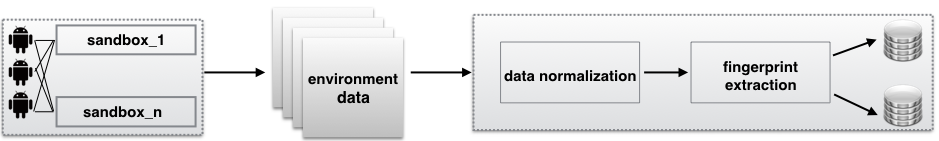
\includegraphics[keepaspectratio=true, width=1\textwidth]{system_design_001.png}
\caption{The design of fingerprint collector}
\label{fig:design}
\end{figure*}

\begin{figure}[h!]
\centering
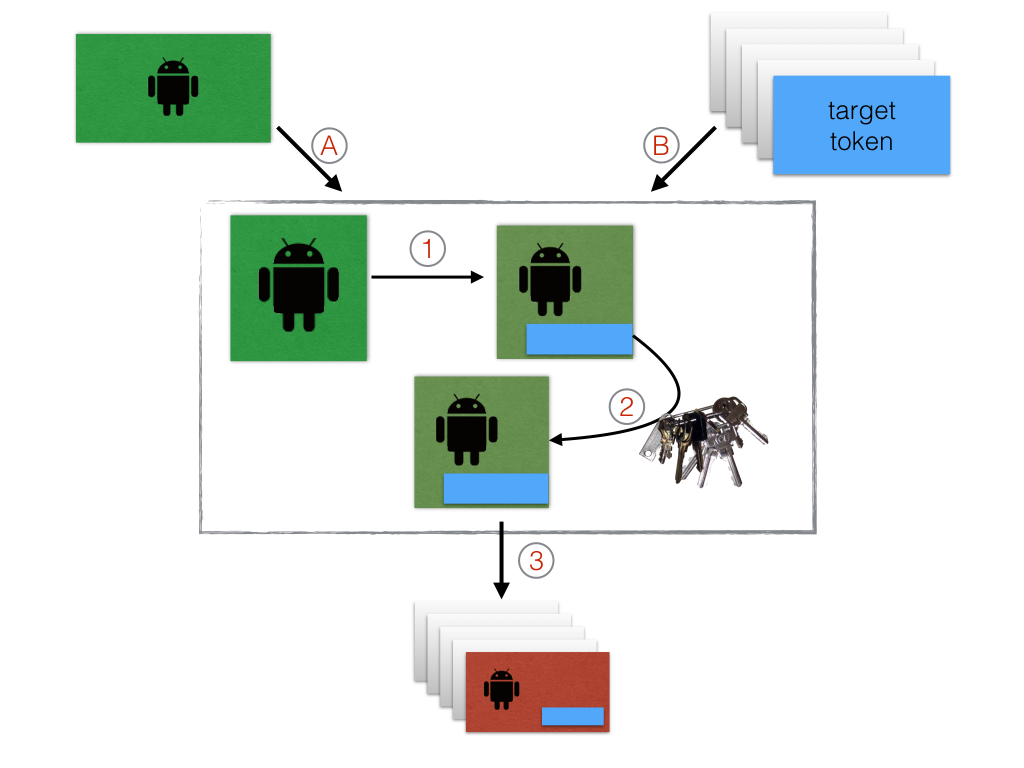
\includegraphics[keepaspectratio=true, width=\columnwidth]{scouter.png}
\caption{Scouting apps generator}
\label{fig:scouter}
\end{figure}

In this section, we present the design of the fingerprint collector. As depicted in Figure \ref{fig:design}, it consists of two components: (I) scouting-app and (II) fingerprint extractor. The scouting-app is used to collect usage-profile fingerprints. It uses only public Android APIs to get information about the execution environment. The app does not use native code, neither Java reflection nor code obfuscation techniques to hide its sensitive behaviors. The reason is that the prior static analysis in most analyzers would highly regard the scouting app as a benign app and filter it out if none suspicious evidence is found. To this end, and to make the fingerprint process even more stealthy as well we implemented several scouting-app each testing for a subset of usage-profile we were interested in. By following this approach we avoid to create a single application that requires a lot of sensitive privileges which could be marked as suspicious and then manually analyzed later on, instead we use several scouting-app such that none of those would require a suspicious combination of sensitive privileges.  \\
The scouting app uses different threads to execute the scouting logic. Each analysis sends its results back to the remote server in the JSON format. All types of collected fingerprints are shown in Table \ref{tab:data}. \\
% Differently from other works \cite{neuner2014enter}, where  sandbox detection uses by low level information like execution time
% All the collected data is strongly related to run-time environment \\

\begin{table}
\centering
\caption{ usage-profile Data }
\begin{tabular}{|c|c|} \hline
Type&Data\\ \hline
Contact & Name, numbers, email\\ \hline
Location & GPS, network, latitude, longitude \\ \hline
%Sensors & power, maxrange, resolution, vendor, version \\ \hline
SMS & inbox, send, draft\\ \hline
%System & fs, ps, uname, mount, df \\ \hline
WiFi & SSID, signal-strength  \\ \hline
App & package-name, version, hash \\ \hline
Battery & battery-level, stat, chargePlug \\ \hline
Call & recent calls \\
%Debugger & /proc/ , isDebuggerConnected \\ 
\hline
\end{tabular}
\label{tab:data}
\end{table}

To track which sandbox analyzes the scouting app, we need to build a scouting app generator. In the scouting app generator, we use a testing app as the base app to generate different apps for each target sandbox. Each generated app is signed by a different certificate. We also make the signature of each app different to avoid the trivial caching mechanism used by the sandbox. Moreover, since we need to classify the results coming back from the testing app, we repackaged the testing app for inserting a \textit{target token}. Then, at run-time the app sends back that token within its fingerprint data. Besides that, the app also sends back its certificate signature, so that we can check if the app has been repackaged by the sandbox for using the static instrumentation hooking framework. Advanced sandbox might employ mechanisms in order to fool the certificate signature check, to countermeasure those we included Java code which is responsible for calculating the DEX file hash value at runtime. With these checks in place, we can detect sandbox which eventually have modified the application being analyzed in order to disable signature checks. 

Figure \ref{fig:scouter} shows the generator design: the system receives the testing app (A) and a list of \textit{target tokens} (B) as inputs. Then, for each target token the generator performs repackaging of the testing app by inserting the target token (1) in app's assets directory. Then, a new digital certificate is created and the repackaged app is signed with. This procedure repeats for each target token. Finally, the output is a set of apps which contain a token for each different target sandboxes.


The fingerprint extractor component first does normalization on the results collected by our scouting applications. It then stores the unique data in a database and uses the token mechanism to create the mapping between the scouting app and the target sandbox. Finally, the collected data is analyzed to determine whether the produced data from the sandbox is dynamically generated or not.
\section{Results} 
\label{sec:res}
In this section, we describe the fingerprints collected by the scouting app. 
Because of the difference in the Android app distribution channel, 
we choose different types of mobile sandboxes accordingly as the target of this work, which are shown in the Table \ref{tab:sandbox}. In fact, it is composed by both official and third-party stores, i.e. Google Play, aptoide, F-Droid, etc\ldots
and also by stock applications installed on real-world devices. First column in Table \ref{tab:sandbox} shows the type of sandbox being analyzed, second and third columns represent sandbox's name and its availability at the time of writing respectively.
We choose to target mobile anti-virus vendors because they use either their own customized sandboxes or an online sandbox service to dynamically analyze collected samples. Moreover, we collect the environment-related data from third-party stores, because it is one of the most popular malware spreading channel. Considering that online malware analysis services are used by both mobile anti-virus and third-party stores, we also collect environment-related data from available online sandboxes. Unfortunately, compared to other previous works \cite{vidas2014evading,petsas2014rage,neuner2014enter,spreitzenbarth2013mobile}, we find that just few of these online services are available at the time of writing, as evicted by third column of Table \ref{tab:sandbox}.

We use the system described in Section \ref{sec:design} to generate 10 applications for each target sandbox. Then, depending of the target type, we manually upload each generated app by using the web interface provided by the online sandbox service, or install on a real device or send it to the third-party store. In the latter case, we immediately remove the app as soon as the scouting app has been analyzed to make sure nobody has ever downloaded it. Moreover, we do not disclose the mapping between the sandbox name and its representing label to allow to sandbox maintainers to fix this problem.


\begin{table}
\centering
\caption{Mobile Sandboxes employed for evaluation. (\xmark\  means not available at the time of writing)}
\begin{tabular}{|c|c|c|} \hline
Type&Sandbox&Available\\ \hline
\multirow{6}{*}{Online} & Andrubis \cite{weichselbaum2014andrubis} & \xmark \\ 
& SandDroid \cite{botnet2014sanddroid} & \cmark \\ 
& TraceDroid\cite{van2013dynamic} & \xmark \\ 
& CopperDroid\cite{tam2015copperdroid} & \xmark \\ 
  & HackApp \cite{apphack} & \xmark \\
& NVISO ApkScan \cite{nviso}& \cmark \\ 
& Koodous  \cite{koodus}& \cmark \\
& VirusTotal \cite{total2012virustotal}& \cmark \\
& Joe Sandbox mobile \cite{joesandbox} & \cmark \\
& ForeSafe & \xmark \\ \hline
\multirow{2}{*}{Antivirus} & Bit Defender & \cmark \\
& 360 mobile & \cmark \\ 
& TrendMicro & \cmark \\
& Kaspersky & \cmark \\ 
& Tencent mobile & \cmark \\ 
\hline
\multirow{1}{*}{App store} & Amazon \cite{amazon} & \cmark \\
\hline
\end{tabular}
\label{tab:sandbox}
\end{table}

We receive the environment-related data from 80\% of available sandbox in the Table \ref{tab:sandbox}. Table \ref{tab:contact} and Table \ref{tab:sms} show a summary of the most relevant environment-related data collected by our testing app. The former contains results of Contact data while the latter contains results of SMS data. Both Tables have the last two columns in common which report whether the specific sandbox does dynamically generates the environment-related data (Random data column) and count the number of collected results (num. of results column) respectively. As for Table \ref{tab:contact} we reported name, number and email were collected by the analysis, instead in Table \ref{tab:sms} we included sending number and body if any. We have not included the phone call data since all sandboxes return the empty result. Thus, the phone call data could be one of the best user-profile fingerprints. 

As describe in Section \ref{sec:design}, our system allows us to detect if a target sandbox returns a fixed data for a specific \textit{environment artifact}. Unfortunately, as shown by "Random Data" column in Table \ref{tab:contact} and \ref{tab:sms}, the results indicate that most Android sandboxes do not use dynamically generated environment data.

One interesting finding is that two mobile anti-virus sandboxes ran the application on a real-world device. In fact, they returned concrete \\
\textit{Wi\-Fi artifact} data (i.e. "wifiscan":"DIRECT\-Cn\-FireTV\_8048",\\
"wifiscan":"AppStore","wifiscan":"AVcontrol"). \\
Moreover, the data collected from the \textit{battery artifact}, presented in Table \ref{tab:battery} is exactly the same for all the sandbox, except for the data returned by these two anti-virus sandboxes. In fact, an unmodified Android emulator returns a fixed battery stats, which consists of the following string: \\
"chargePlug":"1","batteryStat":"2","batteryLevel":"50.0". \\
Instead, results collected from a real-world device look like different: \\
"chargePlug":"2", "batteryStat":"3", "batteryLevel":"100.0". \\ 
Regarding \textit{application artifact} data, we found that about 77\% of targets the sandboxes contain the identical set of applications found on stock Android emulator. As Tables \ref{tab:apps} shown, some anti-virus and all online sandboxes present only the default installed app list from the Android emulator, and they never return random data for the installed app list. \\

In the following list, we include some interesting apps' package name:

\begin{itemize}
\item com.amazon.geo.contextcards
\item com.amazon.rialto.cordova.webapp. 	\\	webapp50f95ccb054443059066310aefdf969b 
\item IAPV2AndroidSampleAPK
\item com.amazon.otaverifier
\item com.tencent.token
\end{itemize}




\begin{table*}
\centering
\caption{Contacts usage-profile Results}
\begin{tabular}{|c|c|c|c|c|c|} \hline
Sandbox & Name & Phone & Email & Random data & num. of results\\ \hline
\multirow{2}{*}{store\_1} & Mary Edwards & 867-5309 & \xmark & 
\multirow{+2}{*}{\xmark} & \multirow{+2}{*}{2}\\
& Harry Grace & 867-5319 & \xmark & &\\ \hline
online\_x & \xmark & \xmark & \xmark & \multirow{+1}{*}{\xmark} & \multirow{+1}{*}{1} \\ \hline	
\multirow{+3}{*}{online\_y} & Firstname1 & 1 301-234-5678 & \xmark &
\multirow{+3}{*}{\xmark} & \multirow{+3}{*}{3}\\
& Firstname2 & 1 381-234-5678 & \xmark & &\\
& Firstname3 & 1 381-234-5678 & \xmark & &\\ \hline
\multirow{3}{*}
{av\_1} & Ion & 074-354-3219  &  \xmark & 
\multirow{+2}{*}{\xmark} & \\
& Gheo & 072-345-6789 & \xmark & & 4 \\ 
& Txet4321 & 074-212-3456 & \xmark & & \\ \hline
\multirow{4}{*}
{av\_2} & Cynthia & \xmark & \xmark &
\multirow{+4}{*}{\xmark} & \multirow{+4}{*}{2}\\ 
& Alexander  & \xmark & \xmark & & \\ 
& Alexandra & \xmark & \xmark & & \\
& Dolores & \xmark & \xmark & & \\ \hline 
\multirow{1}{*}{av\_3}& MARS & 1 566-666-6666 & chengkai\_tao@****.com.cn &
\multirow{+1}{*}{\xmark} & \multirow{+1}{*}{10}\\ \hline
\multirow{3}{*}{av\_4} & Boulder Hypnotherapy Ctr & (303) 776 8100 & z**y@gmail.com & 
\multirow{+3}{*}{\cmark} & \multirow{+3}{*}{36}\\
& St. John Ambulance & 061 412480 & l**k@stjohn.ie& &\\
& Maidstone Golf Centre & 01622 863163 & nick@totalgolfcoaching.co.uk & &\\  \hline
\multirow{3}{*}{av\_5} & Jian Li & 1 3743888229 & lijxev@admin.cn & 
\multirow{+3}{*}{\cmark} & \multirow{+3}{*}{20}\\
& Jian Li & 13606500401 & b0***54@admin.cn & &  \\
& Xuri Jin & 13250324837 & 55**43@yuepao.cn & &\\ \hline
\end{tabular}
\label{tab:contact}
\end{table*}


\begin{table*}
\centering
\caption{SMS usage-profile Results}
\begin{tabular}{|c|c|c|c|c|} \hline
Sandbox & Num  & Body & Random data & num. of results\\ \hline
\multirow{3}{*}{store\_1} & 2020845845 & Hey & 
\multirow{+3}{*}{\xmark} & \multirow{+3}{*}{3}\\
& +18454119384  & Who &  &\\
& 5618675309  & Important & &\\ \hline
\multirow{1}{*}{online}& 
\xmark & \xmark & \xmark & \multirow{+1}{*}{1}\\ \hline	
\multirow{2}{*}{av\_1} & 12345 & smsmomealain & \multirow{+2}{*}{\xmark} & \multirow{+2}{*}{2}\\
& 1234 & smsmomealain  & & \\ \hline
\multirow{2}{*}{av\_2} & 1354-587-2365 & Mum & 
\multirow{+2}{*}{\xmark} & \multirow{+2}{*}{2}\\ 
& 1857-667-8565 & Jefferson& &\\  \hline
\multirow{3}{*}{av\_3} & 1301-234-5678 & Ggggggggg & 
\multirow{+3}{*}{\xmark} & \multirow{+3}{*}{12}\\
&1301-234-5678 & Testzzzzzz &  &\\
&1381-234-5678 & 123456789& &\\ 
&1581-234-5678 & Fffffffffmmmmmm & &\\ \hline
\multirow{4}{*}{av\_4} & 10668820 & guchulaichonghuafei &
\multirow{+4}{*}{\cmark} & \multirow{+4}{*}{15}\\ 
& 10086  & nihao,laikaitong4g-songliuliango & &\\ 
& 13770837893  & nihao,nishi4staryonghu,keyihuantingji & &\\ \hline 
\multirow{3}{*}{av\_5}&13540877911&u0oydyemvub4lu86kfcbwad46pvhmh6o & \multirow{+3}{*}{\cmark} & \multirow{+3}{*}{22}\\ 
&15874984303 & 2fqjfkr629blowmxso4jh6dzqtk3f4j2 & &\\
&18660928896 & lhb0j8hxi48wdjiua1q0qvsleeffgt6g & &\\
\hline
\end{tabular}
\label{tab:sms}
\end{table*}


\begin{table*}
\centering
\caption{Battery usage-profile Results}
\begin{tabular}{|c|c|c|} \hline
Sandbox & Battery stats & Random data  \\ \hline
av\_1 & batteryStat'='3, 'chargePlug'='2', batteryLevel = '100' & \cmark  \\ \hline
av\_2 & batteryStat'='2, 'chargePlug'='1', batteryLevel = '98' & \cmark  \\  \hline
online, store & batteryStat'='2','chargePlug'='1','batteryLevel'= '50.0' & \xmark \\ 
\hline
\end{tabular}
\label{tab:battery}
\end{table*}

\begin{table*}
\centering
\caption{Installed Apps usage-profile Results}
\begin{tabular}{|c|c|c|c|} \hline
Sandbox & Emulator apps & uncommon apps  & Random data\\ \hline
av\_x & \cmark & \cmark & \xmark \\ \hline
av\_y & \cmark & \xmark & \xmark \\ \hline
store & \cmark & \cmark & \xmark \\ \hline
online & \cmark & \xmark & \xmark \\ 
\hline
\end{tabular}
\label{tab:apps}
\end{table*}



\section{Defense}
\label{sec:defense}
As we discussed in previous sections, the environment-related data represents an interesting source of information, which could be exploited to identify the mobile sandbox. Building a database of fingerprints from all sandboxes, an attacker could take the advantage to easily detect an existing mobile sandbox by checking the presence of matching data in the running environment.

To avoid this trivial detection mechanism, it is important to generate environment-related data dynamically, so each application under analysis would see a different environment.

Note that the presence of each previous discussed \textit{environment artifact} is also an important indicator of the goodness of the running environment. As discussed in Section \ref{sec:res}, sandboxes have not included the \text{Call artifact}. Even though such type of environment data i.e. Wi\-Fi data, could not be generated, one can artificially inject it by using hooking frameworks introduced in previous works \cite{costamagna11artdroid, Xposed,Cydia,AndroidHooker}.

In addition to set up the sandbox environment as close as a real user phone, the sandbox developer could take a hybrid approach to detect such fingerprint collection behavior. For example, some sandboxes are equipped with the same set of environmental data, and other sandboxes are equipped with complete different data. When performing the dynamic analysis, each suspicious sample should be run in these two different sandboxes with similar triggering events. If two types of sandboxes yield different malicious behaviors, it indicates that the malware performs the evasion attack by checking the usage-profile based fingerprints.
\section{Related Work}
\label{sec:related}

In this section, we will review existing solutions related to our work in light of the requirements listed above. 

Enforcing customised security policies in stock Android devices is quite challenging. In fact, stock Android does not offer any runtime mechanisms for a third-party app to monitor and trace actions of other apps. Due to secure isolation offered by Android's UID-based sandboxing mechanism, apps can not elevate their privilege to root to monitor other apps that are running under a different UID, e.g., like AV programs are allowed to do on a desktop OS. Consequently, most available solutions for stock Android versions are limited to userspace-available mechanisms for monitoring and enforcing security policies restricting app's behaviour. \\
We summarized related approaches proposed in the literature in Table \ref{tab:comp} and classify them according to whether they satisfy or not our requirements. 

Early works for enforcing security and privacy  policies  \cite{wang2015deepdroid,conti2010crepe,enck2014taintdroid,russello2013firedroid,heuser2014asm,bugiel2011practical} proposed to modify part of the Android OS (both at Java and native levels) or required root privilege. On the one hand they meet many of our requirements: they do not require access to the app code; the sandbox mechanism per-se does not require more permission than the app it monitors; they are able to support both Java and native monitoring levels; they have negligible overhead.
%and they do not affect the usability as the monitored apps can properly go through an update process  R7:\ding{52}). 
However,  they require modifications to the Android codebase making it impossible to deploy them on stock devices. 

To address these limitations, researches proposed sandbox solutions based on rewriting the bytecode of the apps using inline reference monitors (IRM) to enforce security policy. Third column of Table \ref{tab:comp} shows those approaches \cite{xu2012aurasium,you2016reference,zhou2015hybrid} that have support for both Java and native monitoring layers.
Although these systems work on stock Android, they present several limitations when it comes to rewrite obfuscated apps  as reported by previous research \cite{hao2013effectiveness}. Furthermore, once they modify the APK of the target app they break the developer copyright. On the other hand, they do not require any additional permission and they have low impact on performances.



\newcolumntype{L}[1]{>{\raggedright\let\newline\\\arraybackslash\hspace{0pt}}m{#1}}
\newcolumntype{C}[1]{>{\centering\let\newline\\\arraybackslash\hspace{0pt}}m{#1}}


\begin{table*}
\caption{Comparison of Proposed Sandboxing Approaches Based on Desired Requirements. ( \ding{52} = applies; \ding{56} = does not apply )}
\label{tab:comp}
\centering
\ra{1.3}
\begin{tabular}{>{\kern-\tabcolsep}L{.17\linewidth}C{.14\linewidth}C{.15\linewidth}C{.12\linewidth}C{.09\linewidth}g<{\kern-\tabcolsep}}\toprule

Requirements &  OS/root Extension \cite{bugiel2011practical, wang2015deepdroid,conti2010crepe,enck2014taintdroid,russello2013firedroid,heuser2014asm}  & Aurasium\cite{xu2012aurasium} \hspace{0.6cm} Ref. Hijacking\cite{you2016reference} Hybrid\cite{zhou2015hybrid} & Boxify\cite{backes2015boxify} & Njas\cite{bianchi2015njas} & AppBox \\
\midrule
(R1) No root / OS modifications &\ding{56}  & \ding{52} & \ding{52} &  \ding{52} & \ding{52} \\
\hline
(R2) Permissions & \ding{52}  & \ding{52} & \ding{56}   & \ding{52} &\ding{52}	\\
\hline
(R3) Universal & \ding{56} & \ding{56} & \ding{56} & \ding{56} & \ding{52} \\
\hline
(R4) Java and native & \ding{52}  & \ding{52} & \ding{52} & \ding{56} & \ding{52} \\
\hline
(R5) Lightweight &\ding{52} & \ding{52} & \ding{56} & \ding{56} & \ding{52} \\
\bottomrule
\end{tabular}
\end{table*}

More recently, two works have been published that have similar goals of our approach: 
Boxify \cite{backes2015boxify} and NJAS \cite{bianchi2015njas}. Both of these approaches do not need to modify the Android OS and do not require root privileges. 

Boxify offers app virtualization by means of isolated process, a feature introduced in Android 4.1. 
An isolated process is a special process that executes without any privilege. This provides an isolation technique that works on stock Android devices. To manage the permissions required by the monitored apps, Boxify introduces a \textit{Broker}. The Broker to work has to collect the permissions of all the apps monitored in Boxify thus creating a component that has the cumulative privileges of all  sandboxed apps  and introducing a single point of failure. Furthermore, because an isolated process can not use the Android API, Boxify must semantically interpret through the Broker all the Binder parcels an app generates to respect the app's semantic. 

To achieve full patching of all app communications, Boxify must understand the semantics of the apps. This operation generates ovehead and it would be extremely difficult for all obfuscated apps. As side-effect, the Broker introduces an additional hurdle because it needs to emulate critical Android core services (e.g., PackageManager).  
The Broker represents a bottleneck because all the accesses to resources the apps perform have to go though it which has an impact on performance. On the other hand, Boxify offers monitoring capabilities on both Java and native layers. Finally, since the sandboxed apps are not installed in the system, the Android OS can not directly manage them. This means that when an app is updated, the distribution of the new code can not be done automatically as with normal apps but needs the extra effort from the user.

NJAS provides a sandboxing solution based on the PTrace mechanism. NJAS does not require to access the app code to be able to sandbox it and works on stock Android devices. In contrast with Boxify, its monitoring mechanism does not increase the permissions set from the apps. In NJAS the target app is installed on the user device and then executed within a stub app in which it is monitored by means of PTrace. For this reason, NJAS is tightly bound to the availability of PTrace on the user device, thus limiting its deploy-ability on a wide number of real-world mobile devices. As seen in the desktop environment where several Linux distributions removed support for PTrace, this could happen also for the Android system, making impossible to deploy approach such as NJAS.
 
Furthermore, considering the high number of context switches added by the PTrace-based syscall filtering which NJAS uses, it is not a lightweight solution. Finally, it enforces policies only at native level and it does not support Java. NJAS also
requires the user interaction to update the stub component as soon as an update for the managed app is published. 

Samsung Knox  provides a commercial solution. It focuses on providing capabilities including Trusted Boot, TrustZone-based Integrity Measurement Architecture (TIMA), SE for Android, and Knox containers, to protect the Android system from malware and isolate different working scenarios \cite{knox}. Despite that Knox APIs are integrated into Android 5.0 \cite{knox1}, its adoption is limited to Samsung devices \cite{knox2}. Moreover, Knox requires ARM TrustZone hardware support, which limits its deployment to only certain Android platforms.  In contrast, our \asd system is a software-based solution that can be deployed on almost all Android platforms. 

At the beginning of 2015 Google launched Android for Work~\cite{AFW} (AFW), a set of Android device features and services that separate personal apps and data from a work profile containing work apps and data. Google provides APIs for third-party enterprise mobility management (EMM) providers to build Android solutions, Android for Work supports many enterprise use cases but there are two general device deployment scenarios, Bring-your-own-Device (BYOD) and Corporate-owned, single-use (COSU). Android for Work management capabilities rely upon features that are part of newer Android operating system, it is currently supported on devices running Android 5.0 Lollipop and later that support a managed profile\footnote{\url{https://developer.android.com/about/versions/android-5.0-changes.html\#managed_profiles}}. Being enrolled in AFW, a device can be monitored by the IT department that can distribute internal apps on Google Play for Work, a business-specific market offered by AFW. An app that is requested to run in a manged profile must make use of  Android For Work API\footnote{\url{https://developer.android.com/work/guide.html}}, for this reason the developer has to modify the app's codebase (R1:\ding{56}) including those APIs that are requested to communicate with the DPC component. 
\section{Chapter Summary}
\label{sec:conclusion}
In this chapter, we presented a targeted triggering approach, TeICC, to stimulate ICC in Android apps. TeICC is based on backward program slicing which in turn relies on a SDG. The SDG based backward slice extraction technique used by TeICC enables it to extract-then-execute target slices across multiple app components. Moreover, the iterative hybrid approach allows TeICC to extract runtime values (\textit{i.e.,} reflection values, decrypted strings, etc.) to enrich the original app. These runtime values help in performing improved static analysis of obfuscated apps in the next iteration. 

As a future work, we would like to provide support for content providers. Moreover, we focus on different approaches to overcome current limitations. For example, to address the extraction of slices involving native calls, we are analyzing a novel approach using the ARTDroid \cite{costamagnaartdroid} framework to intercept sensitive Java methods called by native code.

\chapter{OctoDroid: Discovering Vulnerability in Android via CPG}

\chapter{StaDART: Combining Static and Dynamic Analysis}
In this chapter, we present StaDART, an extented version of our previously proposed solution Stadyna, which combines static and dynamic analysis of Android applications to reveal the concealed behavior of malware. Unlike Stadyna, StaDART utilizes ArtDroid to avoid modifications to the Android framework. Furthermore, we integrate it with a triggering solution, DroidBot, to make it more scal- able and evaluate it with more Android applications. We present our evaluation results with a dataset of 2,000 real world applications; containing 1,000 legitimate applications and 1,000 malware samples.



\section{Introduction}

Ensuring smartphone users' privacy and security is a major concern and requires adequate measures from app developers, framework providers, and app stores, etc. Google's open source operating system, Android, being the most popular platform for mobile devices, uses Google Bouncer as an app vetting process at its official Google Play store. Vetting processes generally use some form of static/dynamic analysis to scrutinize apps for malicious content and Google Bouncer is no different. In addition, starting from Android 7.0, Android introduced Verify Apps, a new security feature to analyze apps downloaded from sources other than the Google Play store. 

%~\cite{google-bouncer}

However, a growing number of malware samples found in the Android ecosystem reveals that malware developers bypass such vetting processes using various evasion techniques. Previous research shows that the use of dynamic code update techniques along with various forms of obfuscation makes it extremely hard for the state-of-the-art analysis tools to understand the behavior of an app\cite{ExecuteThis_Poeplau2014, ahmad2016empirical}. Thus, the use of these evasion techniques in newly found malware is not surprising~\cite{brain-test}. This paper provides an empirical demonstration of the lack of effectiveness of the state-of-the-art tools when it comes to analysing apps that hide suspicious behavior using reflection and dynamic code loading. We develop a set of benchmark apps that use reflection in different ways to conceal information leakage. Our analysis of reflection-bench using some of the state-of-the-art static analysis tools shows their ineffectiveness to handle apps that use reflection. Furthermore, we develop InboxArchiver, a seemingly benign app that uses dynamic code loading to hide its suspicious functionality, and use it to test some of the most well known online analysis services. The analysis show that InboxArchiver easily bypasses these security analysis services. %\footnote{Similar proof of concept apps, which were able to 

Static analysis relies on the availability of all the information at analysis time, hence, it suffers  from dynamic features and unavailability of information that are known only at execution time, e.g., the parameters used in the dynamic code update APIs. Therefore, reflection that is a programming technique widely used by mobile app developers can be only partially investigated by current  static analysis tools. As a result, reflection is usually used by malware developers to hide malicious code. The inherent limitation of  all static analyzers  (e.g., \cite{FlowDroid_Arzt2014,Saaf_Hoffmann2013}) is the operational assumption  that the code base does not change dynamically and the targets of reflection calls can be discovered in advance. This is a clear simplification of what happens in the real world, where many apps rely on code base updates instantiated only at runtime.


There exist approaches that enhanced static analyzers of Java code to deal with the presence of dynamic code update techniques (e.g., \cite{TamingReflection_Bodden2011}). However, they cannot be  applied directly to Android due to the differences in the Java and Android platforms. The alternative of instrumenting the app offline has the  major drawback of breaking the app signature, that some apps check  at runtime. As the app starts, it checks the integrity of the signature against  a  value hardcoded in the app and terminates if the check fails. In case of malicious apps this check may be used to conceal illicit behavior. 

In this paper, we present StaDART, a mobile app security analysis tool that combines static and dynamic analysis to address the presence of dynamic code updates. Instead of relying on modifications to the Android framework, StaDART utilizes a vtable tampering technique for API hooking to perform dynamic instrumentation~\cite{costamagna2016artdroid}. Furthermore, we integrate StaDART with DroidBot, a triggering tool for Android apps, to make the analysis  fully automated. StaDART is evaluated using a dataset of 2,000 real world apps (both malicious and benign) and the results of our evaluation reveal that it is more common in malicious apps to use dynamic code updates to conceal malicious behavior which is only exhibited once the app is installed on a real device. Moreover, 33\% of malware samples that use DCL introduce APIs guarded with new (not used in the initial code base) dangerous permissions in the newly loaded code, whereas the analysed benign apps do not exhibit such behavior.  

\textbf{Contributions:}

\begin{itemize}
\item We present the design and implementation of StaDART, a system that interleaves static and dynamic analysis in order to reveal the hidden/updated behavior of Android apps. By utilizing vtable tampering for API hooking, we avoid modifications to the Android framework and make it largely framework independent. StaDART analyzes the code loaded dynamically, and is able to resolve the targets of reflective calls complementing app's method call graph with the obtained information. Therefore, StaDART can be used in conjunction with other static analyzers to make their analysis more accurate.

\item We integrate StaDART with DroidBot to make it fully automated and to ease the evaluation. Moreover, we analyze a dataset of 2,000 real world apps (1,000 benign and 1,000 malicious). Our analysis results show the effectiveness of StaDART in revealing behavior which is otherwise hidden to static analysis tools.  

\item We release our tool as open-source to drive the research on app analysis in the presence of dynamic code updates.
%\footnote{\url{new link}}
\item We design and develop reflection-bench, a set of benchmark apps that use reflection to conceal information leakage, and use it to test some of the state-of-the-art static analysis tools. We publish reflection-bench so that researchers can test the effectiveness of their analysis tools in the presence of dynamic features (i.e., reflection). 

\end{itemize}

\textbf{Paper Organization:}

\S\ref{sec:info_android} provides a background on dynamic class loading and reflection in Android. 
\S\ref{sec:refbench_dcl} discusses the design and implementation details of reflection-bench and InboxArchiver. It also provides the analysis results highlighting the shortcomings of state-of-the-art Android app analysis tools. \S\ref{sec::system_general_description} gives a high-level description of StaDART, while \S\ref{sec::implementation} covers the implementation details. \S \ref{sec:mcg_description} presents our approach to build method call graphs and visualise them. \S\ref{sec:evaluation} reports the evaluation results of StaDART on real world apps. \S\ref{sec:discussion} discusses the limitations of the current implementation, and envisages the future work. \S\ref{sec:relwork} overviews the related work, and \S\ref{sec:conclusion} concludes the paper.



\chapter{Conclusions and Future Work}




% ********************************** Back Matter *******************************
% Backmatter should be commented out, if you are using appendices after References
%\backmatter

% ********************************** Bibliography ******************************
\begin{spacing}{0.9}

% To use the conventional natbib style referencing
% Bibliography style previews: http://nodonn.tipido.net/bibstyle.php
% Reference styles: http://sites.stat.psu.edu/~surajit/present/bib.htm

\bibliographystyle{apalike}
%\bibliographystyle{unsrt} % Use for unsorted references  
%\bibliographystyle{plainnat} % use this to have URLs listed in References
\cleardoublepage
\bibliography{References/references} % Path to your References.bib file


% If you would like to use BibLaTeX for your references, pass `custombib' as
% an option in the document class. The location of 'reference.bib' should be
% specified in the preamble.tex file in the custombib section.
% Comment out the lines related to natbib above and uncomment the following line.

%\printbibliography[heading=bibintoc, title={References}]


\end{spacing}

% ********************************** Appendices ********************************

%\begin{appendices} % Using appendices environment for more functunality

%%!TEX root = ../thesis.tex
% ******************************* Thesis Appendix A ****************************
\chapter{} 

\section*{List of Publications}

\subsection*{TeXLive package - full version}
\begin{enumerate}
\item	Download the TeXLive ISO (2.2GB) from\\
\href{https://www.tug.org/texlive/}{https://www.tug.org/texlive/}
\item	Download WinCDEmu (if you don't have a virtual drive) from \\
\href{http://wincdemu.sysprogs.org/download/}
{http://wincdemu.sysprogs.org/download/}
\item	To install Windows CD Emulator follow the instructions at\\
\href{http://wincdemu.sysprogs.org/tutorials/install/}
{http://wincdemu.sysprogs.org/tutorials/install/}
\item	Right click the iso and mount it using the WinCDEmu as shown in \\
\href{http://wincdemu.sysprogs.org/tutorials/mount/}{
http://wincdemu.sysprogs.org/tutorials/mount/}
\item	Open your virtual drive and run setup.pl
\end{enumerate}

or

\subsection*{Basic MikTeX - \TeX~ distribution}
\begin{enumerate}
\item	Download Basic-MiK\TeX (32bit or 64bit) from\\
\href{http://miktex.org/download}{http://miktex.org/download}
\item	Run the installer 
\item	To add a new package go to Start >> All Programs >> MikTex >> Maintenance (Admin) and choose Package Manager
\item	Select or search for packages to install
\end{enumerate}

\subsection*{TexStudio - \TeX~ editor}
\begin{enumerate}
\item	Download TexStudio from\\
\href{http://texstudio.sourceforge.net/\#downloads}
{http://texstudio.sourceforge.net/\#downloads} 
\item	Run the installer
\end{enumerate}

\section*{Mac OS X}
\subsection*{MacTeX - \TeX~ distribution}
\begin{enumerate}
\item	Download the file from\\
\href{https://www.tug.org/mactex/}{https://www.tug.org/mactex/}
\item	Extract and double click to run the installer. It does the entire configuration, sit back and relax.
\end{enumerate}

\subsection*{TexStudio - \TeX~ editor}
\begin{enumerate}
\item	Download TexStudio from\\
\href{http://texstudio.sourceforge.net/\#downloads}
{http://texstudio.sourceforge.net/\#downloads} 
\item	Extract and Start
\end{enumerate}


\section*{Unix/Linux}
\subsection*{TeXLive - \TeX~ distribution}
\subsubsection*{Getting the distribution:}
\begin{enumerate}
\item	TexLive can be downloaded from\\
\href{http://www.tug.org/texlive/acquire-netinstall.html}
{http://www.tug.org/texlive/acquire-netinstall.html}.
\item	TexLive is provided by most operating system you can use (rpm,apt-get or yum) to get TexLive distributions
\end{enumerate}

\subsubsection*{Installation}
\begin{enumerate}
\item	Mount the ISO file in the mnt directory
\begin{verbatim}
mount -t iso9660 -o ro,loop,noauto /your/texlive####.iso /mnt
\end{verbatim}

\item	Install wget on your OS (use rpm, apt-get or yum install)
\item	Run the installer script install-tl.
\begin{verbatim}
	cd /your/download/directory
	./install-tl
\end{verbatim}
\item	Enter command `i' for installation

\item	Post-Installation configuration:\\
\href{http://www.tug.org/texlive/doc/texlive-en/texlive-en.html\#x1-320003.4.1}
{http://www.tug.org/texlive/doc/texlive-en/texlive-en.html\#x1-320003.4.1} 
\item	Set the path for the directory of TexLive binaries in your .bashrc file
\end{enumerate}

\subsubsection*{For 32bit OS}
For Bourne-compatible shells such as bash, and using Intel x86 GNU/Linux and a default directory setup as an example, the file to edit might be \begin{verbatim}
edit $~/.bashrc file and add following lines
PATH=/usr/local/texlive/2011/bin/i386-linux:$PATH; 
export PATH 
MANPATH=/usr/local/texlive/2011/texmf/doc/man:$MANPATH;
export MANPATH 
INFOPATH=/usr/local/texlive/2011/texmf/doc/info:$INFOPATH;
export INFOPATH
\end{verbatim}
\subsubsection*{For 64bit OS}
\begin{verbatim}
edit $~/.bashrc file and add following lines
PATH=/usr/local/texlive/2011/bin/x86_64-linux:$PATH;
export PATH 
MANPATH=/usr/local/texlive/2011/texmf/doc/man:$MANPATH;
export MANPATH 
INFOPATH=/usr/local/texlive/2011/texmf/doc/info:$INFOPATH;
export INFOPATH

\end{verbatim}



%\subsection{Installing directly using Linux packages} 
\subsubsection*{Fedora/RedHat/CentOS:}
\begin{verbatim} 
sudo yum install texlive 
sudo yum install psutils 
\end{verbatim}


\subsubsection*{SUSE:}
\begin{verbatim}
sudo zypper install texlive
\end{verbatim}


\subsubsection*{Debian/Ubuntu:}
\begin{verbatim} 
sudo apt-get install texlive texlive-latex-extra 
sudo apt-get install psutils
\end{verbatim}

%%!TEX root = ../thesis.tex
% ******************************* Thesis Appendix B ********************************

\chapter{}

\LaTeX.cls files can be accessed system-wide when they are placed in the
<texmf>/tex/latex directory, where <texmf> is the root directory of the user’s \TeX installation. On systems that have a local texmf tree (<texmflocal>), which
may be named ``texmf-local'' or ``localtexmf'', it may be advisable to install packages in <texmflocal>, rather than <texmf> as the contents of the former, unlike that of the latter, are preserved after the \LaTeX system is reinstalled and/or upgraded.

It is recommended that the user create a subdirectory <texmf>/tex/latex/CUED for all CUED related \LaTeX class and package files. On some \LaTeX systems, the directory look-up tables will need to be refreshed after making additions or deletions to the system files. For \TeX Live systems this is accomplished via executing ``texhash'' as root. MIK\TeX users can run ``initexmf -u'' to accomplish the same thing.

Users not willing or able to install the files system-wide can install them in their personal directories, but will then have to provide the path (full or relative) in addition to the filename when referring to them in \LaTeX.

%\end{appendices}

% *************************************** Index ********************************
\printthesisindex % If index is present

\end{document}
